\documentclass[times, utf8, diplomski, numeric]{fer}
\usepackage{booktabs}

\usepackage{url}
\usepackage{pdfpages}
\usepackage{subcaption}
\usepackage{listings}
\usepackage[toc,page]{appendix}

\usepackage{listings}
\lstset{
breaklines=true,
basicstyle=\ttfamily}

\renewcommand{\lstlistingname}{Skripta}

\graphicspath{ {images/} }

\newcommand{\eng}[1]{(engl. \textit{#1})}

\begin{document}

\thesisnumber{1385}

\title{Implementacija kontinuirane isporuke programske podrške za operacijski sustav iOS}

\author{Ivan Rep}

\maketitle

% Ispis stranice s napomenom o umetanju izvornika rada. Uklonite naredbu \izvornik ako želite izbaciti tu stranicu.
\izvornik

% Dodavanje zahvale ili prazne stranice. Ako ne želite dodati zahvalu, naredbu ostavite radi prazne stranice.
\zahvala{}

\tableofcontents

\chapter{Uvod}

Profesionalna izrada iOS programske potpore za iOS operacijski sustav zahtjeve čestu isporuku različitih verzija aplikacije. Osim isporuke produkcijske verzije programske potpore čija učestalost može varirati od nekoliko puta tjedno do jednom u nekoliko mjeseci, u sklopu razvoja se isporučuju i druge verzije kao što su verzija za testiranje, verzija koja prikazuje trenutno stanje razvoja i pripremna produkcijska verzija. Učestalost isporuke navedenih tipova također značajno varira od tima do tima.

Kako je iOS operacijski sustav relativno mlad, isporuka se još uvijek uglavnom obavlja ručno. Ručna isporuka programske potpore je vremenski zahtjevna te je podložna ljudskoj pogrešci. Zbog navedenog se izbjegava često obavljanje isporuke što dovodi do zajedničke isporuke većeg broja promjena što zatim dovodi do većeg broja pogrešaka, lošije kvalitete programske potpore te sporije isporuke novih funkcionalnosti.

Ovaj problem je moguće riješiti automatizacijom cijelog ili većeg dijela isporuke programske potpore za iOS operacijski sustav. Međutim, kako bi isporučili programsku potporu, prvo ju moramo arhivirati te zatim dobivenu arhivu objaviti na željenoj platformi. Arhiviranje je proces pripreme iOS projekta za isporuku. Dodano, i proces arhiviranja i proces objave značajno ovise o platformi na kojoj objavljujemo programsku potporu.

Prije arhiviranja programske potpore je istu potrebno izgraditi te utvrditi da zadovoljava sve postavljene uvjete. Uvjeti se najčešće izražavaju u obliku testova ali mogu poprimiti i druge oblike.

Na kraju, potrebno je utvrditi pomoću kojeg je tipa isporuke potrebno isporučiti pojedinu verziju programske potpore.

Navedene funkcionalnosti možemo svrstati u tri dobro prihvaćene prakse u sklopu računalnog inženjerstva: kontinuiranu integraciju, kontinuiranu dostavu i kontinuiranu isporuku.

Kontinuirana integracija automatizira procese izgradnje, testiranja i osiguranja kvalitete prvenstveno kako bi poboljšala kvalitetu programske potpore. Ovako automatizirani proces se provodi nad svakom novom verzijom programske potpore čime se osigurava njena ispravnost. Dodatno, kontinuirana integracija potiče učestalu integraciju radnih kopija s glavnom kopijom kako bi se izbjegla pojava konflikt pri integraciji.

Kontinuirana dostava automatizira proces isporuke programske potpore. U sklopu razvoja programske potpore za iOS operacijski sustav, praksa uključuje automatizaciju potpisivanja koda, arhiviranja i objave. Praksa automatiziranjem navedenih procesa nastoji olakšati proces isporuke te time povećati učestalost objave novih funkcionalnosti. Svaka funkcionalnost koja je razvijena a nije objavljena predstavlja gubitak timu. Dokle god razvijena funkcionalnost sjedi neobjavljena, ona ne donosi korist zbog koje je razvijena. Dodatno, pokazano je da isporuka manjeg broja promjena pozitivno utječe na kvalitetu isporučene programske potpore.

Kontinuirana isporuka nastoji što više smanjiti vrijeme koje protekne od završetka razvoja do objave funkcionalnosti, pa ga čak i u potpunosti eliminirati. Kontinuirana isporuka ovo ostvaruje automatskom isporukom promjena. Međutim, promjene se ne isporučuju direktno u produkciju već prolaze više faza isporuke. Prvo se isporučuju razvojnom timu, zatim timu za osiguranje kvalitete, vanjskim testerima a nekad čak i ograničenom broju stvarnih korisnika. Tek nakon svih ovih faza se promjena isporučuje u produkciju. Kontinuirana integracija ovime nastoji povećati kvalitetu programske potpore, ubrzati isporuku promjena te smanjiti opterećenje razvojnog tima.

U sklopu ovog rada definiram i implementiram navedene prakse za iOS operacijski sustav.

Cilj rada nije samo u teoriji ispitati mogućnost implementacije navedenih procesa, već ih iskoristiti na stvarnim projektima. Zbog navedenog, implementacija mora biti jednostavno prenosiva na drugi projekt. Zbog ovog ograničenja ne samo da nastojim automatizirati isporuku, već nastojim automatizirati i proces dodavanja automatske isporuke iOS projektu.

Rad je strukturiran po praksama u redoslijedu koji je korišten u ovom uvodu. Svaku od praksi prvo promatram iz opće perspektive te zatim definiram i implementiram za iOS operacijski sustav. Rad završava pregledom ostvarenih funkcionalnosti i kratkim zaključkom.


\chapter{Kontinuirana integracija} \label{header:Kontinuirana_Integracija}

Kontinuirana integracija je praksa spajanja razvojnih kopija koda s glavnom kopijom nekoliko puta dnevno. Termin je prvi predložio i iskoristio Grady Booch 1991. godine tijekom opisa metode danas poznate kao Boochova metoda \eng{Booch method}\citep{wiki:BoochMethod}.

Glavni cilj metode je smanjivanje broja konflikata prilikom spajanja različitih verzija koda. Tijekom razvoja članovi tima preuzimaju zajedničku \eng{master} kopiju izvornog koda \eng{source code} te nad njom obavljaju promjene. Lokalnu kopiju izvornog koda nazivamo \textit{razvojnom kopijom izvornog koda}. Članovi tima pomoću zajedničke kopije izvornog koda stvaraju razvojnu kopiju izvornog koda na vlastitom računalu.

Nakon implementacije željenih promjena programer vlastitu razvojnu kopiju spaja s izvornom kopijom. Ovaj postupak nazivamo integracija izvornog koda. Ako zajednička kopija izvornog koda nije bila mijenjana od kako ju je programer preuzeo, onda je promjene moguće jednostavno dodati zajedničkoj kopiji. Međutim, ako je zajednička kopija izvornog koda izmijenjena, onda je potrebno na neki način spojiti lokalne i promjene koje se već nalaze na glavnoj kopiji izvornog koda.

Što je duže programerova kopija izdvojena, to je veća vjerojatnost da je izvorna kopija u međuvremenu izmijenjena. Što se kopije više razlikuju to je teže obaviti njihovo spajanje. Dodatno, spajanje često nije moguće obaviti automatski. Ova se pojava naziva konflikt te se javlja prilikom spajanja kopija koje su istovremeno modificirale isti dio istog dokumenta. Programer u takvom slučaju prvo mora preuzeti novu glavnu kopiju, ručno otkloniti konflikte koje prouzrokuju njegove promjene, te nakon toga obaviti integraciju.

Nakon nekog vremena izvorna i radna kopija mogu postati toliko različite da je vrijeme potrebno za njihovo spajanje duže od vremena koje je uloženo za implementaciju promjena. Ovaj se problem tada naziva \textit{pakao integracije}. Iako se navedena situacija čini teško, mogućom timovi mogu biti veliki, pritisak može biti visok i tempo naporan. Bez specificiranja postupka verzioniranja te automatizacije izgradnje i provjere ispravnosti projekti lako mogu završiti upravo u navedenom stanju.

Danas je kontinuirana integracija standardna praksa u razvoju programske potpore. Međutim, ona se značajno razlikuje od prakse koju je 1991. godine predložio Grady Booch. Danas se uz kontinuiranu integraciju usko vežu procesi automatizacije izgradnje i testiranja programske potpore. Ovi pojmovi su postali toliko standardan dio kontinuirane integracije da mnogi upravo njih nazivaju kontinuiranom integracijom. Drugim riječima, pojam kontinuirane integracije danas podrazumijeva barem neku razinu automatizacije procesa izgradnje i testiranje. S druge strane, učestalom spajanju radnih kopija se daje malo pozornosti.

Kontinuiranu integraciju je moguće podijeliti na tri generalne faze: izgradnju, testiranje i osiguranje kvalitete. Nadalje fazu izgradnje je moguće podijeliti na podfaze verzioniranja, pripreme sustava, pripreme ovisnosti i izgradnje projekta. Faze testiranja i osiguranja kvalitete uvelike ovise o tipu programske potpore koja se razvija. U sklopu ovog rada u fazi testiranja provodim unit i UI testove, dok u sklopu faze osiguranja kvalitete provodim provjeru pokrivenosti koda testovima te provjeru izvornog koda korištenjem alata Swiftlint. Podjela kontinuirane integracije na faze s podfazama je prikazana na slici \ref{fig:CIFazes}.

\begin{figure}
\centering
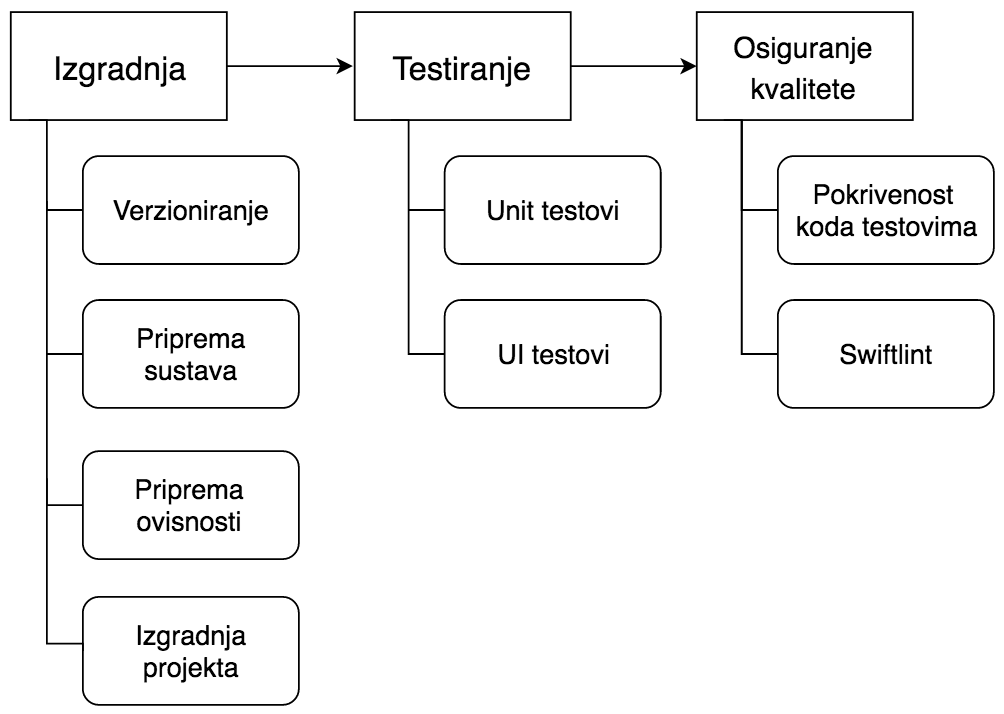
\includegraphics[scale=0.6]{CIFazes}
\caption{Faze kontinuirane integracije}
\label{fig:CIFazes}
\end{figure}

Svaka od faza je obrađena zasebnim odlomkom u nastavku poglavlja. Proces verzioniranja je u praksi dio procesa izgradnje zbog čega je u sklopu odlomka \ref{header:Izgradnja} razmotren i problem učestalosti obavljanja integracije.

Za automatizaciju izgradnje koristim alat Xcode Server. Alat je spoj dvije aplikacije, Xcode i macOS Server te implementira veliki broj funkcionalnosti korištenih u sklopu kontinuirane integracije. Alat se pokazao najboljim među nekoliko sličnih ispitanih alata. Razlog odabira Xcode Server alata je detaljnije prikazan u dodatku \ref{header:dodatak_usporedba_alata_za_kontinuiranu_integraciju}.

\section{Priprema}

Jedan od razloga implementacije kontinuirane integracije je i olakšanje cjelokupnog procesa izgradnje, testiranja i osiguranja kvalitete. Što je implementacije automatizacije zahtjevnija to više narušavam navedeni cilj. Zbog navedenog nastojim automatizirati instalaciju i konfiguraciju što većeg broja alata i time olakšati cjelokupan proces implementacije kontinuirane integracije. Dodatno, automatizacija procesa instalacije i konfiguracije nam omogućava veću kontrolu nad samim procesom. Na primjer, alat je moguće instalirati samo ako je i kad je to potrebno, dok se ručnim postupkom instalacija alata mora obaviti prije pokretanja automatizacije.

Međutim, macOS je vrlo siguran te zbog toga zatvoren operacijski sustav. Veliki broj alata zahtijeva korisničku interakciju zbog čega je njihovu instalaciju teško automatizirati. Ako se instalacija obavlja za više računa ili alat pristupa osjetljivim datotekama onda je instalaciju potrebno autorizirati lozinkom računa s administracijskim privilegijama. Postoji nekoliko načina za automatski upis lozinke, ali navedeni procesi narušavaju sigurnost operacijskog sustava te zbog toga nije moguće u potpunosti automatizirati proces dohvata i pripreme alata.

Ovaj odlomak priprema alate čiju instalaciju nije moguće automatizirati, dok odlomak \ref{header:PripremaSustava} prikazuje pripremu ostalih alata. Primjeri su napisani za macOS operacijski sustav te su testirani na \textit{Sierra 10.12.4} verziji. Minimalna preporučena verzija operacijskog sustava je \textit{Yosemite 10.10}.

Za implementaciju kontinuirane integracije koristim brojne alate koji ne pružaju vizualno korisničkom sučelje. Navedenim se alatima pristupa korištenjem naredbenog korisničkog sučelja - \textit{ljuske}. U sklopu rada koristim \textit{bash} ljusku. Pristup naredbenom korisničkom sučelju se ostvaruje korištenjem emulatora terminala, aplikacija s vizualnim sučeljem koje emuliraju terminal. U radu koristim aplikaciju \textit{Terminal} koja je dostupna u sklopu instalacije macOS operacijskog sustava.

\subsection{Xcode Server}

\begin{figure}
\centering
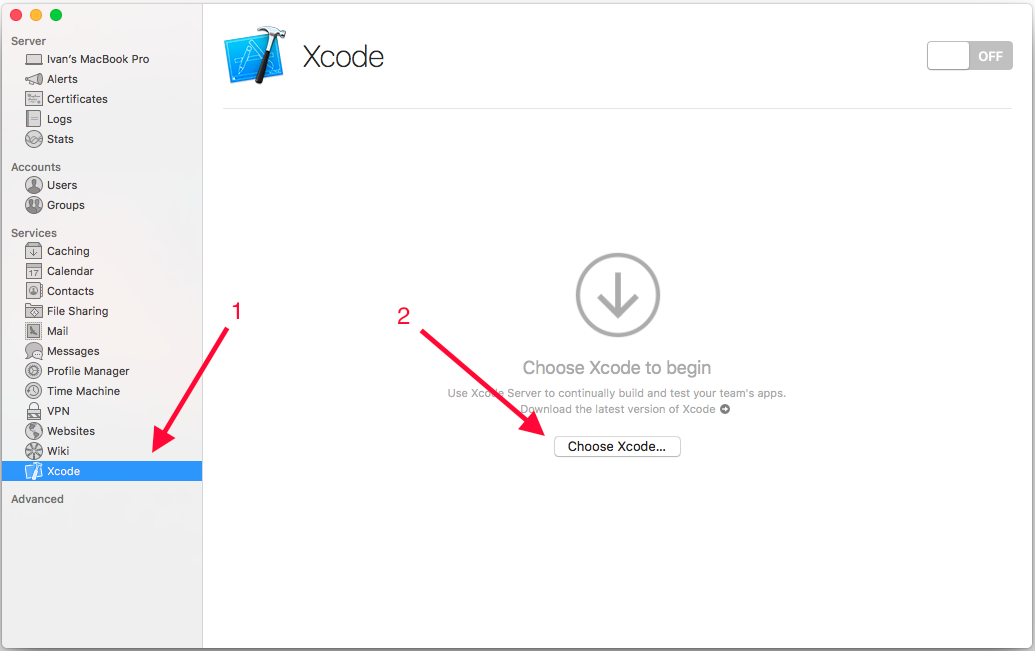
\includegraphics[scale=0.35]{XcodeServerSetup1}
\caption{Povezivanje macOS Server i Xcode aplikacija}
\label{fig:XcodeServerSetup1}
\end{figure}

Xcode Server je spoj dva alata - Xcodea i macOS Servera. Xcode je integrirani sustav razvoj programske potpore za iOS, macOS, tvOS i watchOS operacijske sustave. MacOS Server je alat za automatizaciju procesa na macOS operacijskom sustavu. Prije implementacije kontinuirane integracije je potrebno preuzeti oba alata, instalirati i konfigurirati oba alata.

Oba alata je moguće preuzeti korištenjem App Store aplikacije koje je dostupna u sklopu svake instalacije macOS operacijskog sustava. Međutim, cijena macOS Server aplikacije je u trenutku pisanja ovog rada \$25. Međutim, aplikacija je besplatna za korisnike s Apple Developer računom koji se koristi i u razvoju iOS programske potpore. Besplatnu verziju macOS Servera je moguće preuzeti na poveznici \path{https://developer.apple.com/download/}. Nakon preuzimanja slijediti upute za instalaciju obje aplikacije.

\begin{figure}
\centering
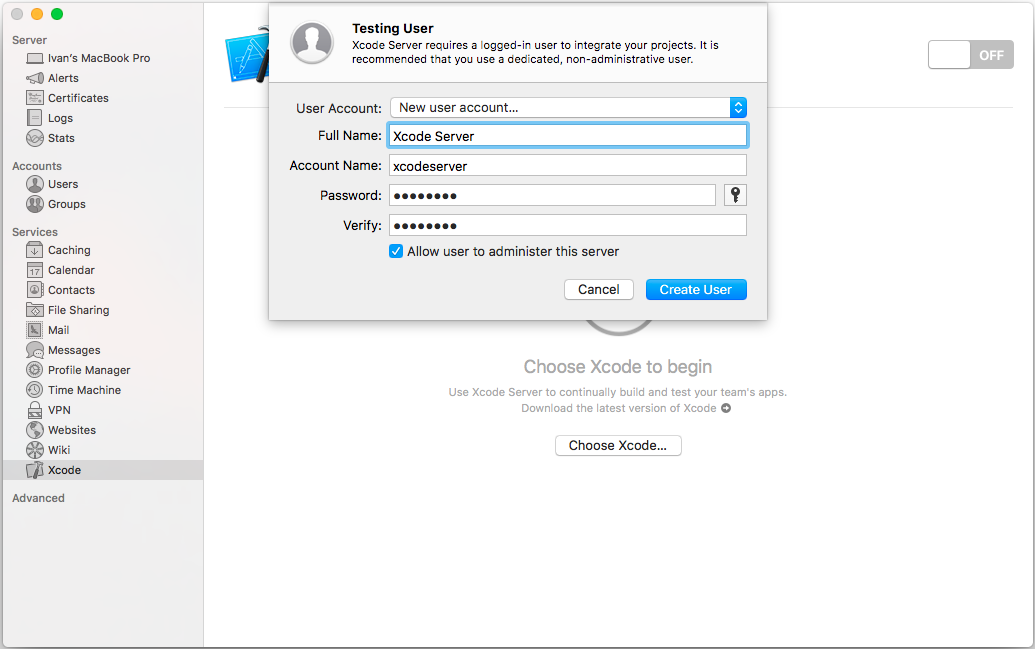
\includegraphics[scale=0.35]{XcodeServerSetup2}
\caption{Kreiranje Xcode Server korisničkog računa}
\label{fig:XcodeServerSetup2}
\end{figure}

Nakon instalacije alata je potrebno kreirati Xcode Server alat povezivanjem Xcode i macOS Server aplikacija. Pokrenuti macOS Server, u lijevom izborniku odabrati \textit{Xcode} te odabrati opciju \textit{Choose Xcode...}. U novo otvorenom izborniku odabrati željenu verziju Xcode aplikacije. Slika \ref{fig:XcodeServerSetup1} prikazuje proces povezivanja macOS Server i Xcode aplikacija.

\begin{figure}[b!]
\centering
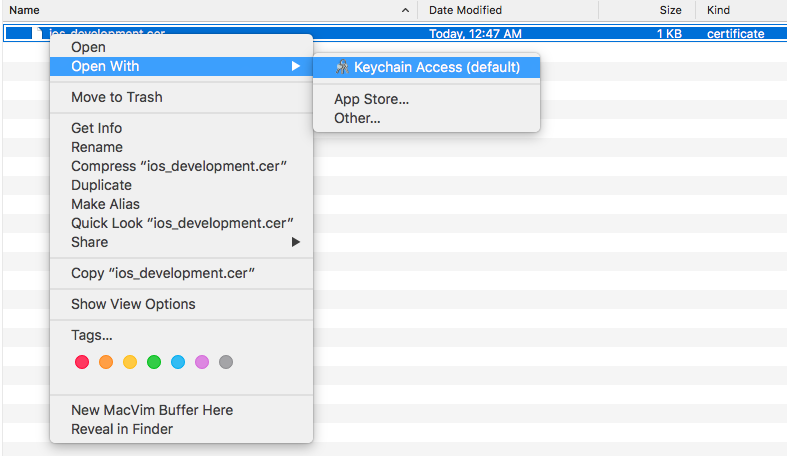
\includegraphics[scale=0.4]{DodavanjeCertifikata}
\caption{Dodavanje certifikata korištenjem Keychain Access aplikacije}
\label{fig:DodavanjeCertifikata}
\end{figure}

Preporučeno je zbog sigurnosnih razloga macOS Server pokrenuti na zasebnom računu operacijskog sustava te omogućiti korištenje samo potrebnih alata i datoteka. Nakon povezivanja Xcode aplikacije s macOS Serverom otvara se izbornik u kojem je moguće kreirati novi račun operacijskog sustava ili odabrati postojeći. U sklopu ovog rada kreiram novi račun predodređenog imena \textit{xcodeserver}. Slijediti upute nakon kreiranja računa za dovršetak spajanja.

Proces potpisivanja koda osigurava autentičnost i neizmjenjenost kreirane programske potpore. Proces je detaljnije objašnjen u \ref{header:PotpisivanjeKoda} odlomku. Za sada je dovoljno znati da proces zahtjeva postojanje tri artefakta: certifikat člana tima, identifikator aplikacije i pripremni profil aplikacije za tip isporuke koji se koristi. Navedene certifikate je moguće kreirati i preuzeti s web stranice \path{https://developer.apple.com/account}.

Certifikat i identifikator se instaliraju korištenjem Keychain Access aplikacije. Dovoljno ih je jednostavno pokrenuti korištenjem navedene aplikacije. Pripremne profile je potrebno spremiti na lokaciji \path{~/Library/MobileDevice/Provisioning_Profiles}.

Xcode Server automatizaciju izgradnje, testiranja i isporuke ostvaruje korištenjem alata nazvanog \textit{bot}. Bot se kreira i konfigurira korištenjem Xcode aplikacije a pokreće na macOS Server aplikaciji. Navedene aplikacije se ne moraju nalaziti na istom računalu ali moraju biti povezane.

Pokrenuti željeni projekt u aplikaciji Xcode. Kreiranje kontinuirane integracije se pokreće odabirom opcije \textit{Product -> Create bot...}.

Nakon odabira navedene opcije otvara se novi prozor u kojem je potrebno imenovati bot te odabrati macOS Server aplikaciju na kojoj će se bot izvršavati. Ukoliko macOS Server nije vidljiv, ponovno pokrenuti macOS Server aplikaciju i provjeriti povezanost s Xcode aplikacijom. Slika \ref{fig:BotServerSelection} prikazuje odabir macOS Server aplikacije kod kreiranja bota.

\begin{figure}
\centering
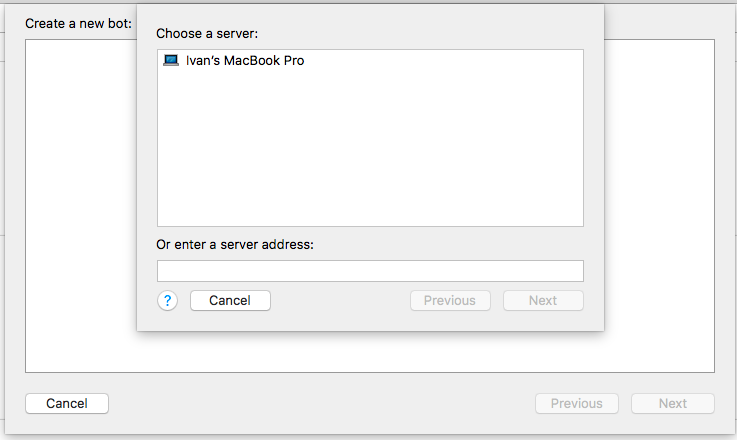
\includegraphics[scale=0.4]{BotServerSelection}
\caption{Odabir macOS Servera aplikacije za obvljanje kontinuirane integracije}
\label{fig:BotServerSelection}
\end{figure}

\subsection{Homebrew}

Homebrew je alat za dohvat i upravljanje alatima za macOS operacijski sustav\citep{homebrew}. Dodatno, alat navedene funkcionalnosti pruža korištenjem naredbenog korisničkog sučelja zbog čega ih je jednostavno automatizirati. Instalacija alata zahtijeva administrativna prava \eng{sudo user}, zbog čega istu nije moguće automatizirati. Skripta \ref{listing:homebrew} instalira Homebrew alat korištenjem alata \textit{ruby}. Nakon pokretanja naredbe slijediti upute instalacije.

\begin{lstlisting}[caption=Instalacija Homebrew alata, label=listing:homebrew]
ruby -e "$(curl -fsSL https://raw.githubusercontent.com/Homebrew/install/master/install)"
\end{lstlisting}

\section{Izgradnja} \label{header:Izgradnja}

Povijesno, pojam izgradnja se često koristio kao sinonim pojma kompajliranje. Kompajliranje \eng{compilation} je proces prevođenja koda iz jednog jezika u drugi uz očuvanje funkcionalnosti. Kod se uz prevođenje često i optimizira . Najčešći razlog kompajliranja je prevođenje koda u jezik kojeg može razumjeti i time izvršiti procesor. Rezultat ovog tipa kompajliranja je izvršni program, odnosno program koji se može izvršiti. Kompajliranje je složena funkcija koja se najčešće obavlja u više prolaza. Jezici koji se kompajliraju se nazivaju kompajlirani jezici \eng{compiled languages}.

Interpretirani jezici \eng{interpreted languages} se ne prevode već interpretiraju. Oni se izvršavaju na pomoćnom programu naziva interpreter koji naredbe izvornog jezika prevodi i izvršava. Danas gotovo niti jedan jezik nije u cijelosti kompajliran ili interpretiran, već koristi kombinaciju obje metode s ciljem poboljšanja performansi.

\begin{figure}[b!]
\centering
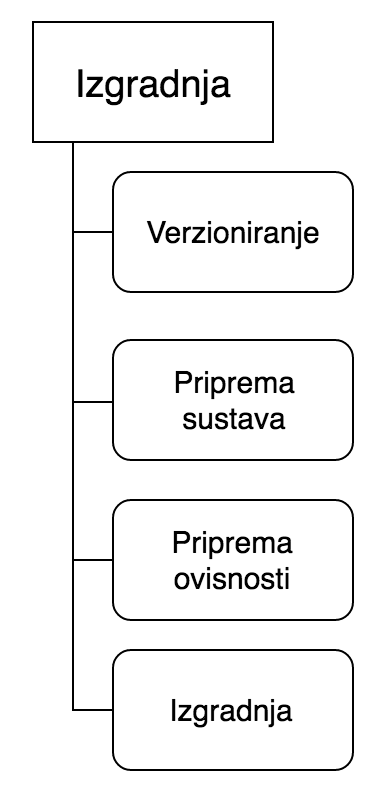
\includegraphics[scale=0.5]{BuildProcess}
\caption{Podfaze procesa izgradnje}
\label{fig:BuildProcess}
\end{figure}

Danas s pojmom izgradnje vežemo sve procese koji su dio pretvaranja izvornog koda u željeni artefakt. Ovisno o jeziku i alatima koje koristimo, proces izgradnje može značajno oscilirati u svojoj veličini. Generalno proces izgradnje možemo podijeliti na verzioniranje, pripremu sustava za izgradnju, dohvat i pripremu ovisnosti \eng{dependancies} te kompajliranje. Verzioniranjem odabiremo željenu verziju izvornog koda koju koristimo za izgradnju artefakta. Priprema za izgradnju dovodi računalo u stanje potrebno za obavljanje izgradnje. Izvorni kod često sadržava upute za pripremu sustava kao što su potrebni alati i postavke projekta. Dohvat i priprema ovisnosti osigurava postojanje ovisnosti koje zahtijeva izvorni kod. Ovisnosti dijelimo na dva tipa, ovisnosti koje su dio razvojne okoline i vanjske \eng{third party} ovisnosti, najčešće razvijene od strane zajednice. Kompajliranje prevodi izvorni kod u izvršivi artefakt. Kod interpretiranih jezika ovaj je proces često zamijenjen statičkom i dinamičkom provjerom izvedivosti programa. Zbog jednostavnijeg sporazumijevanja oba procesa nazivam izgradnja projekta. Slika \ref{fig:BuildProcess} prikazuje podjelu procesa izgradnje.

Osim kreiranja artefakta, izgradnja provjerava i je li zadana verzija izvornog koda izgradiva. Kod je izgradiv ako se u procesu izgradnje ne izaziva pogrešku, odnosno ako se isti ispravno izvrši. Pogrešku može izazvati neispravnost u izvornom kodu, neispravna konfiguracija sustava, nepostojanje potrebnog alata ili neka druga neispravnost. Izgradivost sustava je preduvjet za  testiranja i isporuku. Samim time je automatizacija izgradnje preduvjet za automatizaciju testiranja i automatizaciju isporuke.

\subsection{Verzioniranje} \label{header:Verzioniranje}

Verzioniranje je proces dodjele jedinstvene oznake \eng{id} stanju repozitorija\citep{wiki:SoftwareVersioning}. Repozitorij je verzioniran direktorij te može sadržavati sve od izvornog koda do certifikata i izvršnog programa. Jedinstvena oznaka omogućava identifikaciju pojedinog stanja repozitorija i izgradnju stabla promjena \eng{source tree} koje povezivanjem stanja prikazuje povijest izmjena repozitorija. Verzionirano stanje repozitorija se naziva verzija \eng{commit}.

\begin{figure}[b!]
\centering
\begin{subfigure}{.24\textwidth}
\centering

\includegraphics[scale=0.4]{VersioningTreeA}
\caption{Glavni repozitorij}
\label{fig:VersioningTreeA}
\end{subfigure}
\begin{subfigure}{.24\textwidth}
\centering

\includegraphics[scale=0.4]{VersioningTreeB}
\caption{Repozitorij A}
\label{fig:VersioningTreeB}
\end{subfigure}
\begin{subfigure}{.24\textwidth}
\centering

\includegraphics[scale=0.4]{VersioningTreeC}
\caption{Repozitorij B}
\label{fig:VersioningTreeC}
\end{subfigure}
\begin{subfigure}{.24\textwidth}
\centering
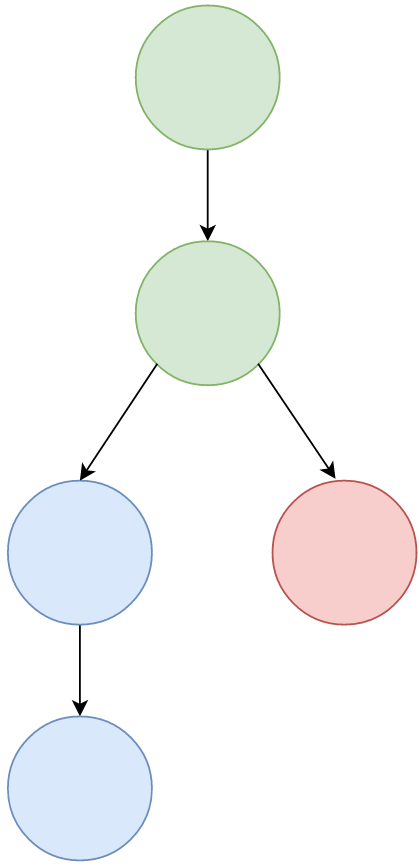
\includegraphics[scale=0.4]{VersioningTree}
\caption{Spojeni prikaz}
\label{fig:VersioningTreeD}
\end{subfigure}
\caption{Stablo promjena}
\label{fig:VersioningTree}
\end{figure}

Uz jedinstvenu oznaku i stanje repozitorija, proces verzioniranja pohranjuje i dodatne podatke kao što su autor i datum kreiranja verzije, te identifikator prijašnje verzije. Navedeni podaci omogućavaju izgradnju stabla promjena. Dodatno, ako verzije poredamo kronološki po datumu obavljanja izmjena, onda svaka pojedina verzija ne treba sadržavati cijelo stanje repozitorija. Dovoljno je samo navesti promjene obavljene nakon prijašnje verzije. Navedeni proces ne samo da značajno smanjuje veličinu cijele kopije, već olakšava i praćenje izmjena. Slika \ref{fig:VersioningTree} prikazuje primjer stabla promjena. Glavni repozitorij sadrži dvije verzije. Repozitorij u navedenom stanju preuzimaju dva člana tima čime kreiraju lokalne repozitorije nad kojima obavljaju izmjene. Globalno stablo promjena se kreira zajedničkim prikazom stabla promjena svih članova.

Navedeni tip verzioniranja se naziva inkrementalno verzioniranje jer se zbog lakšeg praćenje promjena provodi vrlo često. Identifikatori ovog tipa verzioniranja su najčešće generirani pseudo-slučajno. U sklopu razvoja programske potpore najčešće koriste i dodatne sheme verzioniranja koje olakšavaju praćenje stanja projekta. Navedene sheme nastoje olakšati praćenje projekta zbog čega se ovaj tip verzioniranja se naziva vanjsko verzioniranje. Verzije se gotovo uvijek kreiraju dodavanjem posebnih oznaka postojećoj verziji inkrementalnog verzioniranja. Na primjer, u praksi je standardno označiti svaku verziju iz koje se kreira produkt koji se izdaje posebnom oznakom koja se naziva verzija izgradnje \eng{build number}. Kako vanjsko verzioniranje nosi neko značenje, proces dodjele identifikatora je puno složeniji i ovisi o svrsi koje se pokušava postići.

Unutarnje verzioniranje koda se naziva kontrola verzija\citep{wiki:VersionControl}. Sustavi koji implementiraju proces kontrole verzija se nazivaju sustavi za kontrolu verzija. Kroz povijest je razvijen veliki broj sustava za kontrolu verzija te je danas timski razvoj programske potpore gotovo nezamisliv bez korištenja jednog od njih.

Danas su u praksi najpopularnija dva alata: Apach Subversion i git.

Apache Subversion, poznat i pod skraćenicom svn, je kreiran 2000. godine u sklopu projekta vođenog od Apache Software Foundation zajednice. Alat je centraliziran, siguran i jednostavan za korištenje te je danas objavljen kao alat otvorenog koda. Generalno postoji jedan glavni repozitorij kojeg članovi tima kloniraju, uređuju te zatim lokalne promjene sinkroniziraju s glavnim repozitorijem.

Git je kreirao Linus Torvalds 2005. godine zbog nezadovoljstva tadašnjim sustavima za kontrolu verzija. Git je izdan kao alat otvorenog koda te je ubrzo okupio veliku podršku u zajednici. Za razliku od svna, git je distribuirani sustav. Repozitoriji istog projekta mogu postojati na proizvoljnom broju uređaja u proizvoljnom broju stanja. Navedeni se repozitoriji mogu klonirati, usklađivati i uređivati neovisno jedan od drugom. Zbog navedenog je pomoću gita moguće implementirati proizvoljan pristup verzioniranju. Bio to centralizirani repozitorij nalik na svnov pristup, pristup s osobama zaduženim za odobravanje promjena, distribuirani model i drugo. Najvažnije, git je jednostavan ali vrlo moćan alat. Implementacija osnovnih funkcionalnosti je intuitivna dok istovremeno postoji podrška za vrlo kompleksne pothvate.

Svn je stariji, međutim još uvijek široko korišten sustav. Koristi ga veliki broj starijih kompanija i projekata otvorenog koda. Git je značajno popularniji na novijim projektima, posebno onim otvorenog koda. Njegova jednostavnost i fleksibilnost ga čine lakšim za upoznavanje i korištenje. Zbog navedenog u ovom rada koristim git. Sve se funkcionalnosti mogu, uz manju modifikaciju, implementirati i korištenjem svna.


\paragraph{Uvod u git}

Temeljne funkcionalnosti git alata su repozitoriji i grane. Repozitorij je direktorij koji je verzioniran korištenjem git sustava za kontrolu verzija. Ovaj repozitorij sadrži direktorij \verb|.git| koji specificira na koji se način verzionira direktorij te sadrži informacije o repozitoriju.

Repozitoriji se mogu klonirati na istom ili drugom uređaju. Klonirani repozitorij je novi repozitorij identičan izvornom repozitoriju. Promjene koje se obavljaju u kloniranom repozitoriju nemaju nikakvog utjecaja na izvorni repozitorij. Međutim, promjene obavljene u kloniranom repozitoriju se mogu, uz postojanje odgovarajuće autorizacije, prenijeti na izvorni repozitorij. Prijenos promjena se ne mora obavljati isključivo između izvornog i kloniranog repozitorija, već se može obaviti između bilo koja dva povezana repozitorija.

\begin{figure}[b!]
\centering
\begin{minipage}{.5\textwidth}
\centering
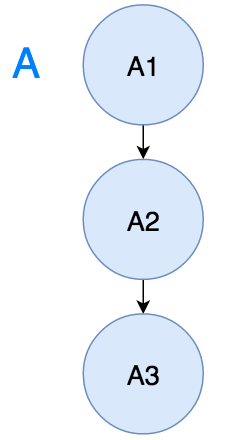
\includegraphics[scale=0.6]{Initial_commit}
\caption{Grana s tri potvrde}
\label{fig:Initial_commit}
\end{minipage}%
\begin{minipage}{.5\textwidth}
\centering
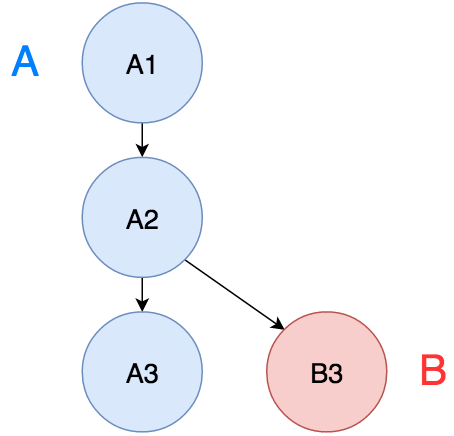
\includegraphics[scale=0.6]{Branching}
\caption{Grananje}
\label{fig:Branching}
\end{minipage}
\end{figure}

Prilikom kreiranja git repozitorija stvara se i glavna grana (eng. master branch) repozitorija. Grana je definirana slijedom verzija koje su obavljene na njoj. Stvaranje nove verzije na trenutnoj grani se ostvaruje potvrđivanjem promjena \eng{commit} koje su dodane repozitoriju. Potvrđivanje promjena je prikazano na slici \ref{fig:Initial_commit}. Repozitorij koda se stvara kreiranjem glavne grane i obavljanjem inicijalnog potvrđivanja \eng{initial commit}. Glavna grana je označena slovom A. Inicijalno potvrđivanje je označeno identifikatorom A1, dok su naknadna potvrđivanja označena identifikatorima A2 i A3.

\begin{figure}
\centering
\begin{subfigure}{.49\textwidth}
\centering
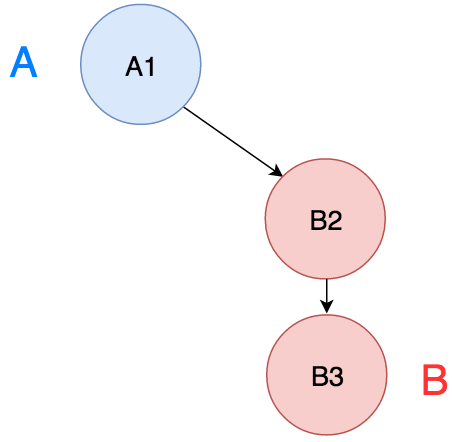
\includegraphics[scale=0.6]{FastForwardA}
\caption{Stanje prije spajanja}
\label{fig:FastForwardA}
\end{subfigure}
\begin{subfigure}{.49\textwidth}
\centering
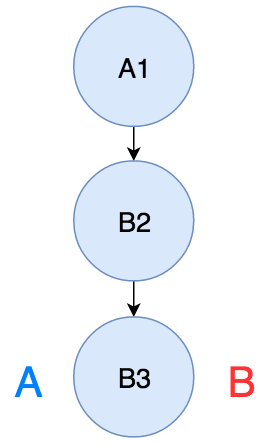
\includegraphics[scale=0.6]{FastForwardB}
\caption{Stanje nakon spajanja}
\label{fig:FastForwardB}
\end{subfigure}
\caption{Spajanje dodavanje promjena}
\label{fig:FastForward}
\end{figure}

Nova grana se može kreirati iz bilo kojeg stanja postojeće granje. Ovaj se postupak naziva grananje \eng{branching}. Izvorna i kreirana grana dijele zajedničku povijest do trenutka grananja. Daljnje promjene se primjenjuju samo na jednu od postojećih grana. Slika \ref{fig:Branching} prikazuje postupak grananja. Grana B se kreira iz stanja A2 grane A. Grane A i B dijele dva zajednička stanja A1 i A2. Ova stanja nazivamo zajednička povijest grana A i B. Nakon grananja na granu B dodajemo novo stanje B3.

Grane je također moguće spojiti. Spajanje grana dodaje promjene obavljene na izvornoj \eng{source} grani u odredišnu \eng{destionation} granu. Spajanje je moguće obaviti na nekoliko načina ovisno o odnosu dviju grana koje se spajaju. Slika \ref{fig:FastForward} prikazuje najjednostavniji odnos dviju grana kod spajanja. Nakon grananja grane B iz stanja A1 grane A na granu B se dodaju dva nova stanja, B2 i B3. U međuvremenu je grana A ostala nepromijenjena. Zbog navedenog je spajanje grana moguće obaviti jednostavno dodavanjem promjena B grane na vrh A grane, \eng{fast forward merge}. Slike \ref{fig:FastForwardA} prikazuje stanje prije spajanja dok slika \ref{fig:FastForwardB} prikazuje stanje nakon spajanja. Dodatno, samo spajanje je moguće označiti dodavanjem novog stanja na odredišnu granu.

Postupak se komplicira ako je odredišna grana modificirana nakon grananja. U navedenom slučaju nije moguće promjene obavljene u izvorišnoj gani samo dodati na vrh odredišne grane, nego je promjene potrebno spojiti. Proces spajanja ovisi o tome postoje li konflikti između promjena. Ako ne postoji, spajanje je moguće obaviti jednako kao na slici \ref{fig:FastForward}, jednostavno dodavanjem promjena na vrh odredišne grane.

\begin{figure}
\centering
\begin{subfigure}{.49\textwidth}
\centering
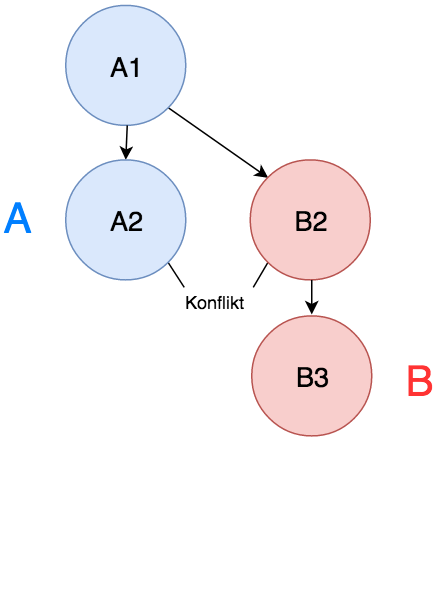
\includegraphics[scale=0.6]{ConflictA}
\caption{Stanje prije spajanja}
\label{fig:ConflictA}
\end{subfigure}
\begin{subfigure}{.49\textwidth}
\centering
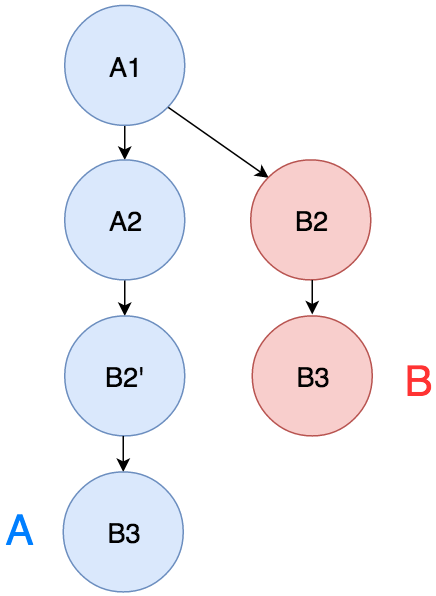
\includegraphics[scale=0.6]{ConflictB}
\caption{Stanje nakon spajanja}
\label{fig:ConflictB}
\end{subfigure}
\caption{Spajanja otklananjem konflikta}
\label{fig:Conflict}
\end{figure}

Međutim, ako promjene izazivaju konflikte, onda je te konflikte potrebno ručno razriješiti. Otklanjanje konflikata uzrokuje izmjenu verzija jedne ili obje grane. Proces otklanjanja konflikata se najčešće odrađuje dodavanjem jedne po jedne verzije izvorne grane na odredišnu granu. Ako dodana verzija ne izaziva konflikt, ona se jednostavno dodaje na vrh odredišne grane. Međutim, ako verzija izaziva konflikt, tada se isti otklanja modificirajući dodanu verziju. Slika \ref{fig:Conflict} prikazuje proces spajanja grana s konfliktom. Konflikt je nastao između verzija A2 i B2. Konflikt se otklanja dodavanjem verzije B2 na vrh A grane i njenim modificiranjem. Ovo je stanje označeno s B2'. Stanje B3 ne izaziva konflikt te se samo dodaje na vrh A grane. Rezultat spajanja su dvije grane A i B različitih povijesti.

\begin{figure}[b!]
\centering
\begin{subfigure}{.3\textwidth}
\centering
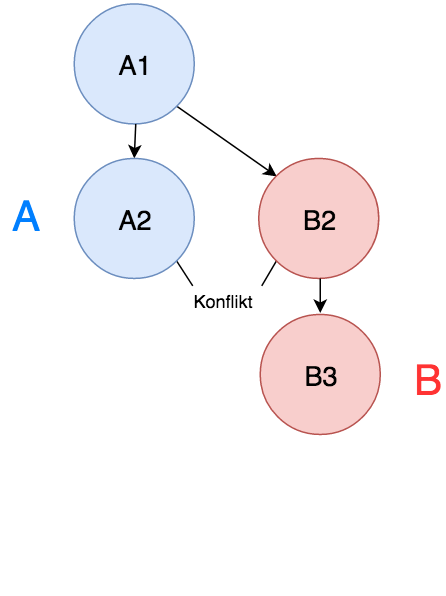
\includegraphics[scale=0.5]{RebaseA}
\caption{Početno stanje}
\label{fig:RebaseA}
\end{subfigure}
\begin{subfigure}{.3\textwidth}
\centering
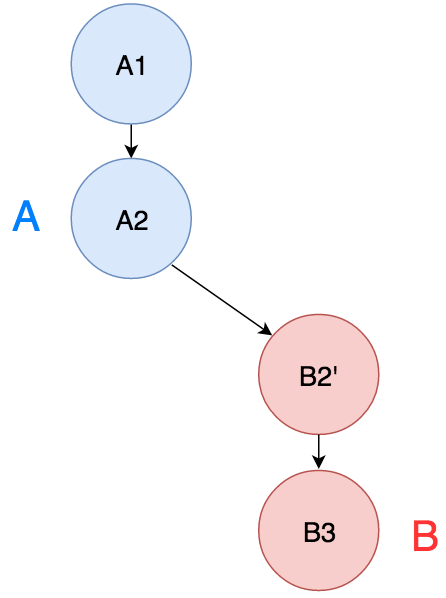
\includegraphics[scale=0.5]{RebaseB}
\caption{Stanje nakon \textit{rebase}}
\label{fig:RebaseB}
\end{subfigure}
\begin{subfigure}{.3\textwidth}
\centering
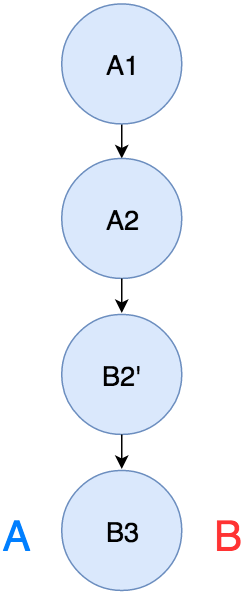
\includegraphics[scale=0.5]{RebaseC}
\caption{Stanje nakon spajanja}
\label{fig:RebaseC}
\end{subfigure}
\caption{Spajanje \textit{rebase} postupkom}
\label{fig:Rebase}
\end{figure}

Isti je slučaj moguće riješiti postupkom koji se naziva \textit{rebase}. Postupak prije spajanja u povijest izvorišne grane dodaje sve verzije nastala u odredišnoj grani nakon grananja. Verzije se dodaju odmah nakon stare točke grananja čime se točka grananja pomiče na zadnju verziju A grane. Slika \ref{fig:RebaseB} prikazuje stanje nakon obavljanja \textit{rebase} postupka na grani B. Sada su grane u stanju jednakom onom na slici \ref{fig:FastForward} te je spajanje moguće obaviti dodavanjem promjena na vrh odredišne grane. Stanje B2 se još uvijek mijenja, međutim sada je povijest repozitorija linearna.


\paragraph{Tijek verzioniranja} \label{header:Implementacija_verzioniranja}

Ostaje otvoreno pitanje kako koristiti alat za kontrolu verzija. Koliko često kreirati novu verziju koda i koliko često promjene spajati sa zajedničkim repozitorijem. Kod korištenja gita se javljaju i pitanja kako organizirati repozitorije i sustav grananja.

Programer koji samostalno radi na projektu najčešće koristi jedan javni repozitorij s jednom granom na kojoj obavlja promjene i proizvoljno sinkronizira lokalni s glavnim repozitorijem. Međutim, ovaj pristup je vrlo teško održiv u timskom radu. Učestalo preplitanje različitih tokova razvoja na jednoj grani značajno otežava praćenje razvoja i čini teškim poništavanje neželjenih promjena.

Danas se u praksi koristi nekoliko različitih tijeka rada verzioniranja \eng{versionining workflows}. Ovaj odlomak obrađuje centralizirani tijek rada \eng{centralized workflow}, tijek rada grananja funkcionalnosti \eng{feature branch workflow}, \textit{gitflow} tijek rada \eng{gitflow workflow} i tijek rada izdvajanja \eng{forking workflow}. Svaki od navedenih pristupa ima svoje prednosti i mane te se koristi u različitim tipovima projekta\citep{versioningWorkflows}.

Centralizirani tijek rada koristi jedan glavni i više lokalnih repozitorija. Najčešće se koristi samo jedna, glavna grana. Svaki programer kreira lokalnu kopiju glavnog repozitorija na kojoj obavlja promjene. Nakon obavljanja željenih promjena iste spaja s glavnom granom centralnog repozitorija. Na pojedinom je programeru da vlastitu, lokalnu verziju repozitorija drži usklađenom s glavnim repozitorijem. Glavni repozitorij predstavlja službeno stanje projekta zbog čega treba posebnu pažnju obratiti na održavanje njegove povijesti. Izmjena povijesti glavnog repozitorija može dovesti lokalne repozitorije u nekonzistentno stanje zbog čega se ona smatra lošom praksom. Zbog navedenog, ako lokalna kopija izaziva konflikt pri spajanju, konflikt je potrebno otkloniti na lokalnoj kopiji te promjene zatim spojiti s centralnim repozitorijem. Centralizirani proces je vrlo jednostavan te je sličan načinu rada svna.

\begin{figure}
\centering
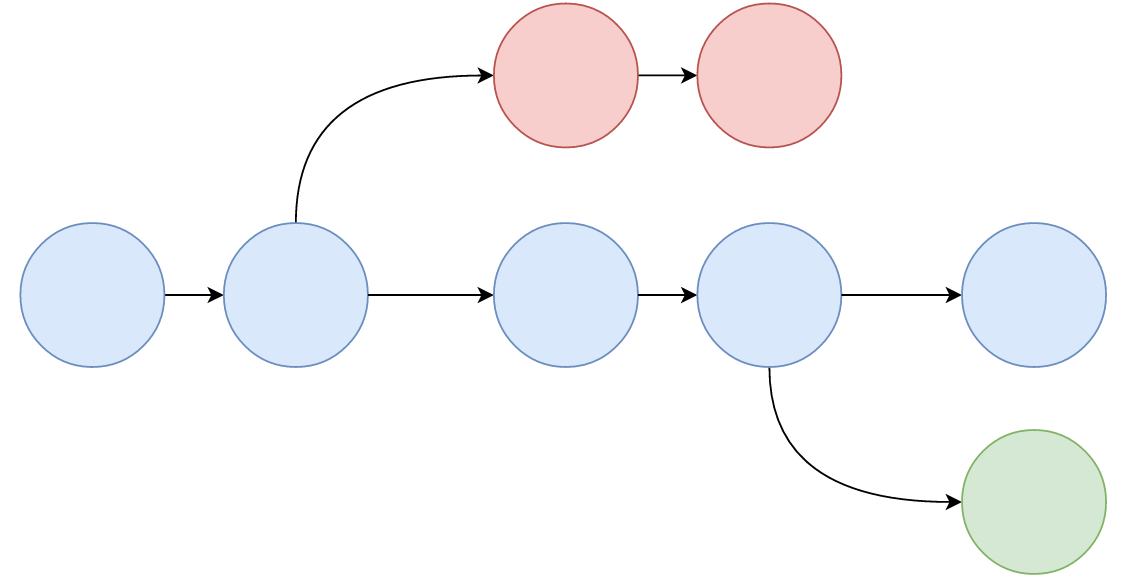
\includegraphics[scale=0.5]{FeatureBranch}
\caption{Primjer tijek rada grananja funkcionalnosti}
\label{fig:FeatureBranch}
\end{figure}

Tijek rada grananja funkcionalnosti nastoji otkloniti glavni nedostatak centraliziranog tijek rada, učestalo preplitanje različitih tokova razvoja. Grananje funkcionalnosti također ima jedan glavni i više lokalnih repozitorija. Razlika je u tome što se funkcionalnost implementira u grani kreiranoj specifično za nju. Programer za novu funkcionalnost kreira novu granu u lokalnom repozitoriju te u nju dodaje promjene. Po završetku implementacije funkcionalnosti programer granu spaja s glavnom granom centralnog repozitorija. Ovaj proces daje jasniji uvid u napredak projekta i implementirane funkcionalnosti. Dodatno, proces timu daje priliku revizije obavljenih promjena. Umjesto direktnog spajanja grane moguće je kreirati zahtjev za spajanjem \eng{merge request}. Zahtjev za spajanjem dodatno opisuje promjene ostvarene u sklopu grane te timu daje priliku za komunikaciju i reviziju obavljenih promjena.

Gitflow tijek rada također koristi jedan centralni i više lokalnih repozitorija. Za razliku od prijašnja dva tijeka rada, gitflow tijek rada povijest repozitorija prati kroz glavnu i razvojnu granu. Razvojna grana \eng{develop branch} je vrlo slična glavnoj grani u procesu grananja funkcionalnosti. Grana za novu funkcionalnost se kreira iz razvojne grane te se po završetku implementacije u nju spaja. S druge strane, glavna grana sadrži samo produkcijske verzije izvornog koda, odnosno one verzije projekta koje su obavljene korisniku. Kad tim odluči objaviti novu verziju projekta, kreira se nova grana iz trenutnog stanja razvojne grane. Nakon završetka provjere ispravnosti grana se spaja s glavnom, i po potrebi razvojnom granom. Nova verzija glavne grane se zatim objavljuje. Verzije na glavnoj grani se označavaju sa objavljenom verzijom projekta.

Primjer korištenja gitflow procesa je prikazan na slici \ref{fig:Gitflow}. Crvenom bojom je prikazana glavna grana a plavom razvoja grana. Grane funkcionalnosti, prikazane zelenom i žutom bojom se granaju iz razvojne grane te u nju spajaju. Bijelom bojom je označena grana pripreme za objavu nove verzije projekta. Nakon obavljanja pripreme za objavu grana se spaja s glavnom granom tima kreirajući novu produkcijsku verziju, te s razvojnom granom kako bi promjene nastale kod pripreme za objavu bile dodane projektu.

\begin{figure}
\centering
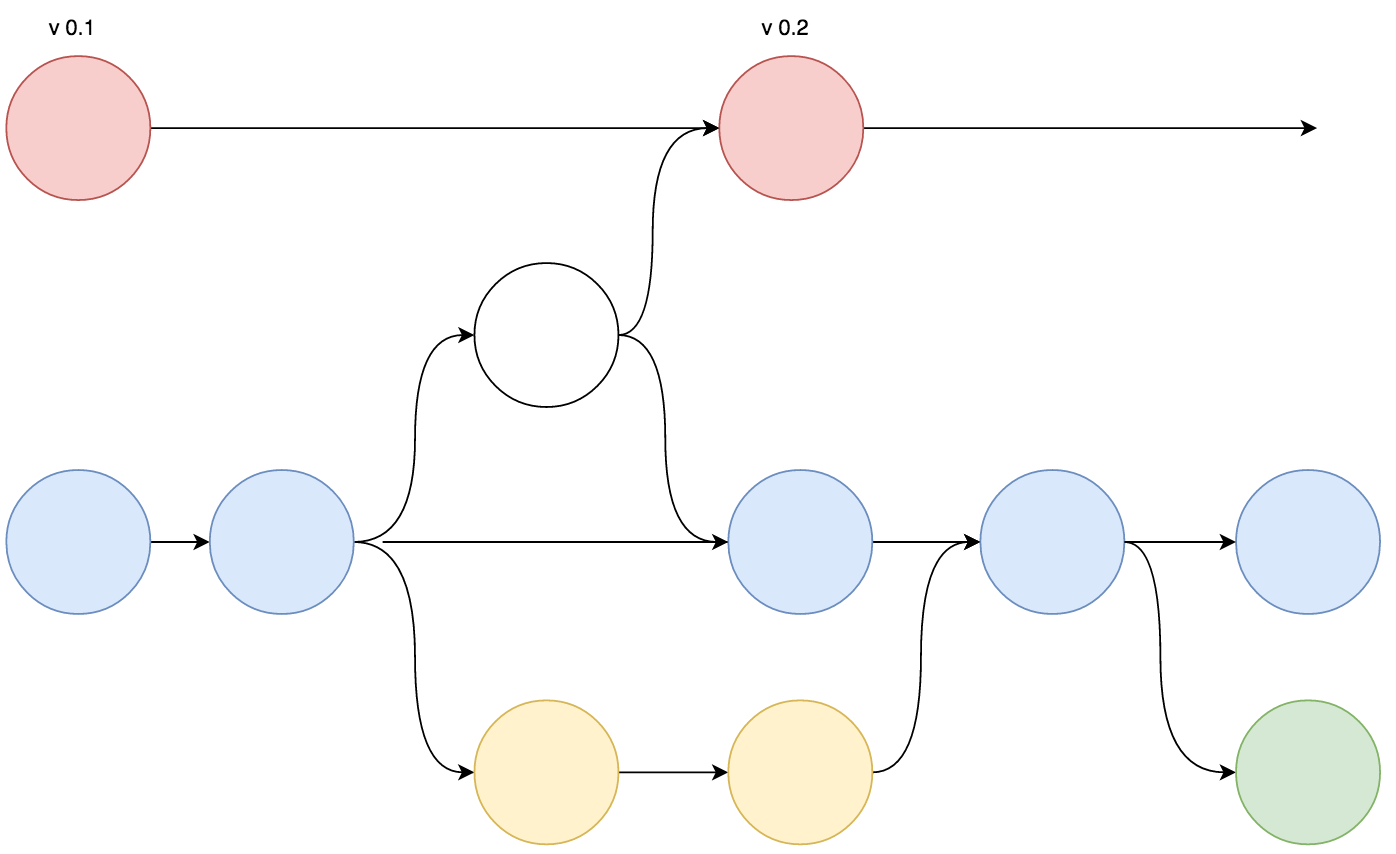
\includegraphics[scale=0.5]{Gitflow}
\caption{Primjer gitflow tijek rada}
\label{fig:Gitflow}
\end{figure}

Navedeni pristup olakšava upravljanje objavom projekta. Buduće da je krucijalno objaviti ispravan produkt sam proces objave treba biti kontroliran i a produkt temeljito testiran. Izdvajajući proces objave na pomoćnu granu omogućava istovremeno testiranje produkcijske verzije i nastavak rada na novim funkcionalnostima.

Za razliku od ostalih tijekova rada promatranih u ovom poglavlju, forking tijek rada nema centralni repozitorij već svaki sudionik ima vlastiti javni i privatni repozitorij. Programer vlastiti javni repozitorij kreira kopiranjem drugog javnog repozitorija. Zatim iz vlastitog javnog repozitorija kreira vlastiti privatni repozitorij. Promjene obavlja na privatnom repozitoriju te ih proizvoljno spaja s javnim repozitorijem. Navedene promjene zatim može iskoristiti netko drugi kloniranjem repozitorija ili spajanjem promjena s postojećim repozitorijem. Dodatno, programer može predložiti dodavanje vlastitih promjena  drugom repozitoriju. Navedeni se proces naziva zahtjev za povlačenjem promjena \eng{pull request}.

Forking tijek rada se najčešće primjenjuje za projekte otvorenog koda. On omogućuje svakom članu zajednice kloniranje, modifikaciju i objavu promjena obavljenih na projektu. Dodatno, zahtjev za spajanje daje vrlo dobar uvid u obavljene promjene bez modifikacije izvornog repozitorija.

Osnova kontinuirane integracije je kontinuirano, odnosno učestalo spajanje radnih kopija s glavnom kopijom. Kad bi se vodili samo ovim principom centralizirani repozitorij bi najbolje zadovoljavao postavljene zahtjeve. Međutim, centralizirani repozitorij se u praksi ne koristi za ništa osim najjednostavnijih projekata.

Iako drugi tijekovi rada rjeđe obavljaju integraciju radnih kopija, prednosti koje pružaju nadilaze navedeni nedostatak. Dodatno, moguće je smanjiti vrijeme između spajanja radnih kopija. Na primjer, gitflow tijek rada spajanje radne kopije s glavnom kopijom obavlja po završetku implementacije funkcionalnosti. Što je veća funkcionalnost koja se implementira, to će duže radna kopija ostati izdvojena. Zbog navedenog je potrebno posao razdijeliti na male dijelove. Navedeno se ne odražava pozitivno samo na proces kontinuirane integracije, već olakšava i praćenje projekta te je sastavni dio agilnog pristupa razvoja programske potpore. Prednosti koje napredniji pristupi verzioniranju pruža, kao što su lakše praćenje razvoja, zahtjevi za spajanjem i lakša objava projekta u produkciju nadilaze nešto duže vrijeme izdvojenosti radnih kopija.

U praktičnom dijelu rada koristim gitflow tijek rada. Ovaj tijek rada najbolje odgovara zahtjevima i tipu projekta. Dodatno, gitflow tijek rada omogućava jednostavniju implementaciju kontinuirane dostave i isporuke. Uz glavnu i radnu granu, repozitoriju ću po potrebi dodavati dodatne grane. Na primjer, isporuku verzija programske potpore za testiranje ću izdvojiti u zasebnu granu. Navedeni proces omogućava lako praćenje testnih verzija te olakšava implementaciju procesa isporuke testne verzije.

\paragraph{Verzioniranje u sklopu kontinuirane integracije}

Proces kontinuirane integracije započinje dohvatom željene verzije repozitorija. Kako bi dohvatio željenu verziju, proces kontinuirane integracije mora imati pristupiti repozitoriju. Xcode Server omogućava korištenje lokalnog ili udaljenog repozitorija verzioniranog svn ili git alatom. Ako se koristi udaljeni repozitorij, onda je isti potrebno zaštiti od neželjenog pristupa. Danas se u praksi koriste dva tipa zaštite: HTTPS i SSH autentifikacija.

HTTPS autentifikacija pristup kontrolira korištenjem jedinstvenog korisničkog imena i lozinke. Budući da se proces integracije odvija automatski, potrebno je spremiti i automatizirati unošenje korisničkog imena i lozinke. Preporučeno je iste pohraniti korištenjem Keychain Access aplikacije.

SSH autentifikacija pristup kontrolira korištenjem javnog i privatnog ključa najčešće generiranog korištenjem RSA protokola. Ova tip autentifikacije je pogodniji za automatizaciju zbog čega ga koristim u sklopu ovog rada. Proces kreiranja i konfiguriranja SSH autentifikacije je detaljnije objašnjen u sljedećem odlomku.

Xcode Server automatski detektira alat kojim je repozitorij verzioniran. Nakon autentifikacije pristupa je potrebno odabrati granu za koju se kreira proces integracije. Pojedini bot integraciju obavlja za samo jednu granu zbog čega je potrebno kreirati zaseban bot za svaku željenu granu. Slika \ref{fig:BotAddingSSH} prikazuje autentifikaciju detektiranog git repozitorija korištenjem postojećeg SSH ključa.

\begin{figure}
\centering
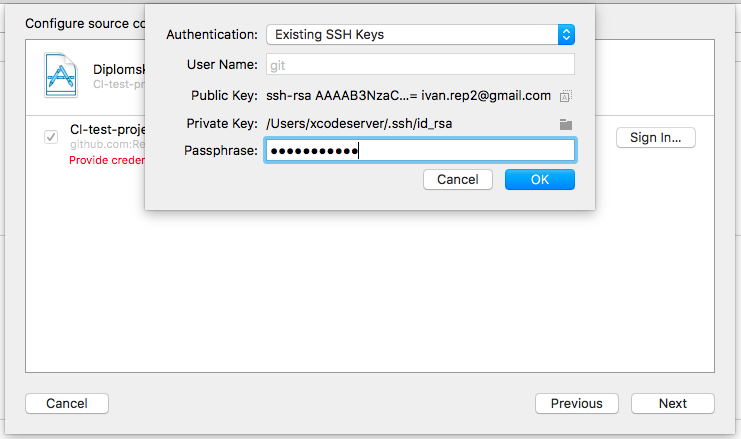
\includegraphics[scale=0.5]{BotAddingSSH}
\caption{Dodavanje SSH ključa}
\label{fig:BotAddingSSH}
\end{figure}

Xcode Server omogućava automatsko pokretanje integracije nakon kreiranja nove verzije na promatranoj grani. Navedenu funkcionalnost Xcode Server ostvaruje kontinuiranom provjerom stanja repozitorija. Proces integracije je također moguće provoditi periodično ili ga pokretati ručno. Slika \ref{fig:CIStartConfig} prikazuje navedene opcije.

\begin{figure}[b!]
\centering
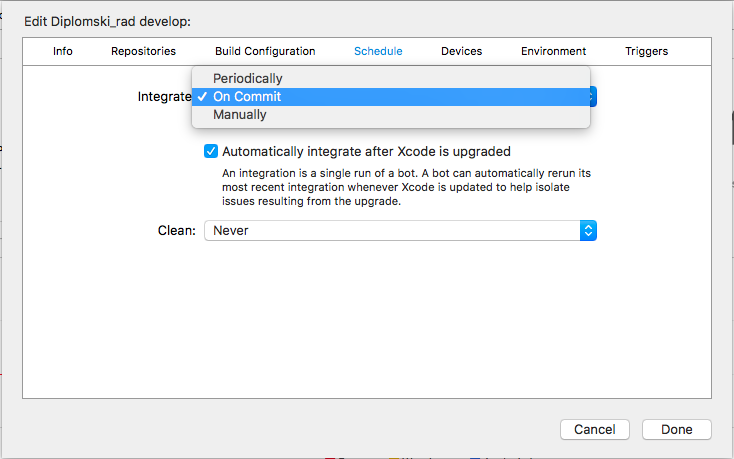
\includegraphics[scale=0.5]{CIStartConfig}
\caption{Odabir načina pokretanja procesa integracije}
\label{fig:CIStartConfig}
\end{figure}

Korištenjem navedenih opcija kontinuirana integracija se pokreće nakon kreiranja novog stanja na odabranoj grani repozitorija.

\paragraph{SSH autentifikacija}

U sklopu rada koristim SSH autentifikaciju za pristup udaljenom git repozitoriju. SSH ključevi se obično pohranjuju u direktoriju \path{~/.ssh}. Ako SSH ključ već ne postoji u navedenom direktoriju, onda potrebno je kreirati isti. Skripta \ref{listing:ssh} prikazuje proces generiranja ključa. Naredba pod \#1 generira novi SSH ključ sa željenom e-mail adresom. Preporučeno je ključ u toku kreiranja zaštiti lozinkom.

Nakon generiranja, ključ je potrebno dodati SSH agentu kako se šifra ključa ne bi morala unositi pri svakom korištenju. Naredbe \#2 i \#3 ostvaruju navedenu funkcionalnost. Na kraju, javni dio ključa je potrebno registrirati na platformi koja hosta repozitorij. Naredba \#4 kopira javni dio novo kreiranog ključa.

\begin{figure}[b!]
\centering
\includegraphics[scale=0.3]{GitHubSSH}
\caption{Dodavanje SSH ključa na GitHub platformu}
\label{fig:GitHubSSH}
\end{figure}

\begin{lstlisting}[caption=Postavljanje SSH autentifikacije, label=listing:ssh]
ssh-keygen -t rsa -b 4096 -C "{e-mail adresa}" #1

eval "$(ssh-agent -s)" #2

ssh-add -K ~/.ssh/{ime_kljuca} #3

pbcopy < ~/.ssh/{ime_kljuca}.pub #4
\end{lstlisting}

U sklopu rada koristim GitHub platformu. Slika \ref{fig:GitHubSSH} prikazuje proces registriranja SSH ključa na GitHub platformi. SSH ključ se dodaje odabirom opcije \textit{Settings -> SSH and GPG keys -> New SSH key} te dodavanjem kopiranog javnog dijela ključa u polje za ključ. Nakon spremanja ključa isti je moguće koristiti za autorizaciju komunikacije s GitHub platformom.


\subsection{Priprema sustava} \label{header:PripremaSustava}

Priprema sustava se sastoji od provjere postojanja, dohvata i konfiguracije potrebnih alata te od pripreme projekta za izgradnju.

Provjeru postojanja alata obavljam korištenjem skripte \ref{listing:PripremaSustavaProvjera}. Naredba \#1 provjerava postojanje alata korištenjem alata \verb|which| koji je dostupan u sklopu instalacija macOS operacijskog sustava. U slučaju nepostojanja alata isti je potrebno dohvatiti i instalirati.

\begin{lstlisting}[caption=Provjera postojanja alata, label=listing:PripremaSustavaProvjera]
if !(which {ime_alata} >/dev/null); then #1
    {naredba za instalaciju alata} #2
fi
\end{lstlisting}

Na navedeni način provjeravam postojanje i instaliram tri alata, alate za dohvat ovisnosti CocoaPods i Carthage, te alat za provjeru ispravnosti koda Swiftlint. Skripta \ref{listing:PripremaSustavaInstalacija} prikazuje automatiziranu instalaciju navedenih alata.


\begin{lstlisting}[caption=Automatizirana instalacija alata, label=listing:PripremaSustavaInstalacija]
if !(which pod >/dev/null); then #1
    echo "Installing CocoaPods"

    gem install cocoapods --user-install
    pod repo update
fi

if !(which carthage >/dev/null); then #2
    echo "Instaling Carthage"

    brew install carthage
fi

if !(which swiftlint >/dev/null); then #3
    echo "Instaling Swiftlint"

    brew install swiftlint
fi
\end{lstlisting}

Naredba pod \#1 provjerava i instalira CocoaPods alat korištenjem alta \verb|gem| dostupnog u sklopu instalacije macOS operacijskog sustava. Kako bi izbjegao unošenje administrativne lozinke, kod instalacije koristim opciju \verb|--user-install| koja alat instalira samo za trenutnog korisnika. Naredbe \#2 i \#3 provjeravaju i instaliraju alate Carthage i Swiftlin korištenjem alata brew.


Konfiguracija Xcode projekta je pohranjena unutar \verb|.xcodeproj| datoteke. Datoteka je namijenjena za modifikaciju i čitanje korištenjem alata Xcode. Datoteka nije pogodna za račnu izmjenu i čitanje. Kako bi se olakšalo nadgledanje i modifikacija postavka projekta često se koriste \verb|xcconfig| datoteke.

Navedene datoteke su tekstualne datoteke s \verb|.xcconfig| nastavkom te sadrže listu \verb|{ključ} = {vrijednost}| linija koje specificiraju postavke projekta. Navedene datoteke je potrebno dodati projektu te iskoristiti za konfiguraciju željene sheme. Pomoću Xcode aplikacije otvoriti projekt te odabrati željenu shemu i sekciju \verb|Info|. U odjeljku \verb|Configurations| odabirom opcije \verb|Plus| kreirati novu konfiguraciju. Slika \ref{fig:XcodeConfigurations} prikazuje proces dodavanja nove konfiguracije.

\begin{figure}[h!]
\centering
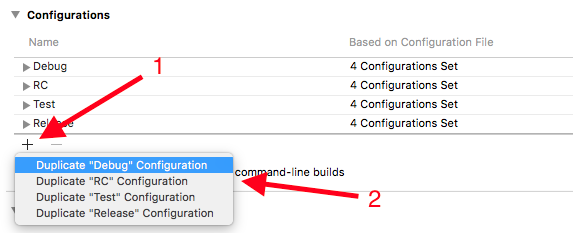
\includegraphics[scale=0.7]{XcodeConfigurations}
\caption{Kreiranje konfiguracije projekta}
\label{fig:XcodeConfigurations}
\end{figure}

Korištenjem novo kreirane konfiguracije odabrati željenu \verb|xcconfig| datoteku.

\subsection{Upravljanje ovisnostima}

Prije izgradnje projekta je potrebno dohvatiti ovisnosti koje projekt koristi. Za dohvaćanje ovisnosti se u iOS razvoju koriste dva alata: \textit{CocoaPods} i \textit{Carthage}. Oba sustava se široko koriste te izbor uvelike ovisi o osobnom ukusu. Zbog navedenog u radu koristim oba alata.

\paragraph{CocoaPods}

CocoaPods je stariji, široko prihvaćen, centraliziran alat za upravljanje ovisnostima iOS projekata. Alat je jednostavan i intuitivan za korištenje. Dovoljno je specificirati ovisnosti korištenjem \verb|Podfile| datoteke i pokrenuti proces dohvata ovisnosti. Alat samostalno kreira i konfigurira radno okruženje te time olakšava proces upravljanja ovisnostima.

Međutim, najveći problem alata je upravo ova učestala modifikacija datoteka radnog okruženja. Alat pri svakom dohvatu izmjenjuje postavke izgradnje što može uzrokovati neželjeno ponašanje. Dodatno, budući da je alat centraliziran, sve korištene biblioteke moraju biti registrirane u CocoaPods sustavu. Navedeno otežava korištenje privatnih biblioteka i biblioteka u razvoju.

Inicijalizacija CocoaPods alata je prikazana u skripti \ref{listing:CocoaPodsInit}. Naredbu je potrebno pokrenuti u direktoriju projekta.

\begin{lstlisting}[caption=Inicijalizacija CocoaPods alata, label=listing:CocoaPodsInit]
pod init
\end{lstlisting}

Naredba kreira \verb|Podfile| datoteku koja služi za specifikaciju ovisnosti. Skripta \ref{listing:PodfileExample} prikazuje primjer \verb|Podfile| datoteke. Datoteka za cilj \verb|Diplomski_rad| specificira dvije ovisnosti \verb|LayoutKit| i \verb|Fabric|.

\begin{lstlisting}[caption=Primjer Podfile datoteke, label=listing:PodfileExample]
use_frameworks!

target 'Diplomski_rad' do
    pod 'LayoutKit'
    pod 'Fabric'
end
\end{lstlisting}

Ovisnosti se dohvaćaju pokretanjem naredbe \verb|pod install| u direktoriju projekta.

Skripta \ref{listing:cocoapods} automatizira dohvaćanje ovisnosti korištenjem CocoaPods alata. Naredba \#1 provjerava postojanja Podfile datoteke te u slučaju postojanja iste nastavlja s izvođenjem skripte. Naredba \#2 provjerava postojanje CocoaPods alata. Ako alat nije instaliran, isti se instalira korištenjem gem alata. Na kraju, naredba \#3 dohvaća ovisnosti korištenjem CocoaPods alata.

\begin{lstlisting}[caption=Dohvat ovisnosti korištenjem alata CocoaPods, label=listing:cocoapods]
if [ -f Podfile ]; then #1
    echo "Podfile found. Starting CocoaPods"

    if ! which pod >/dev/null; then #2
        echo "Installing CocoaPods"

        gem install cocoapods --user-install
        pod repo update
    fi

    pod install #3

    echo "Finished dependancy fetch using CocoaPods"
fi
\end{lstlisting}

\paragraph{Carthage}

Carthage je noviji, decentralizirani alat za upravljanje ovisnostima. Alat omogućava jednostavno dohvaćanje i izgradnju biblioteke bez potrebe njihove prijašnje registracije. Za razliku od CocoaPods alata, Carthage ne modificira radno okruženje. Ovisnosti je potrebno samostalno uključiti u projekt zbog čega je alat složeniji za korištenje od CocoaPods alata. Međutim, u istom trenutku alat otklanja neželjene posljedice koje nosi učestala izmjena datoteka razvojnog okruženja.

Kreirati \verb|Cartfile| datoteku. Datoteka je jednostavna lista ovisnosti zajedno s lokacijom izvornog repozitorija. Skripta \ref{listing:Cartfile} prikazuje primjer \verb|Cartfile| datoteke.

\begin{lstlisting}[caption=Primjer Cartfile datoteke, label=listing:Cartfile]
github "JohnSundell/Unbox"
git "https://gitlab.rep.com/Testni_projekt"
\end{lstlisting}

Primjer dohvaća dvije ovisnosti. Javno objavljenu ovisnost \verb|Unbox| objavljenu na Github platformi te privatnu ovisnost objavljenu na Gitlab platformi.

Dohvaćanje ovisnosti se pokreće naredbom \verb|carthage update|.

Skripta \ref{listing:carthage} implementira dohvaćanje ovisnosti korištenjem Carthage alata. Naredba \#1 provjerava postojanje \verb|Cartfike| datoteke te u slučaju postojanja iste nastavlja obavljanje skripte. Naredba \#2 provjerava postojanje Carthage alata te ga dohvaća ako ne postoji. Naredba \#3 dohvaća ovisnosti korištenjem Carthage alata. Za bolje performanse operacije koristim dva argumenta. Argument \verb|--platform ios| specificira dohvaćanje ovisnosti samo za iOS platformu. Argument \verb|--cache-builds| dohvaća ovisnosti samo ako iste nisu već dostupne.

\begin{lstlisting}[caption=Dohvat ovisnosti korištenjem alata Carthage, label=listing:carthage]
if [ -f Cartfile ]; then #1
    echo "Cartfile found. Starting Carthage"

    if !(which carthage >/dev/null); then #2
        echo "Instaling Carthage"

        brew install carthage
    fi

    carthage update --platform ios --cache-builds #3

    echo "Finished dependancy fetch using Carthage"
fi
\end{lstlisting}

\paragraph{Automatizacija dohvaćanja ovisnosti}

Obje skripte je potrebno pokrenuti prije obavljanja integracije. Za ostvarenje navedene funkcionalnosti botu dodajem skriptu koja se izvršava prije pokretanja integracije \eng{Pre-Integration Script}. Slika \ref{fig:PreIntegrationScript} prikazuje proces dodavanja nove skripte. Skripta se dodaje odabirom opcije \textit{Edit Bot... -> Triggers -> Pre Integration Script}.

\begin{figure}[b!]
\centering
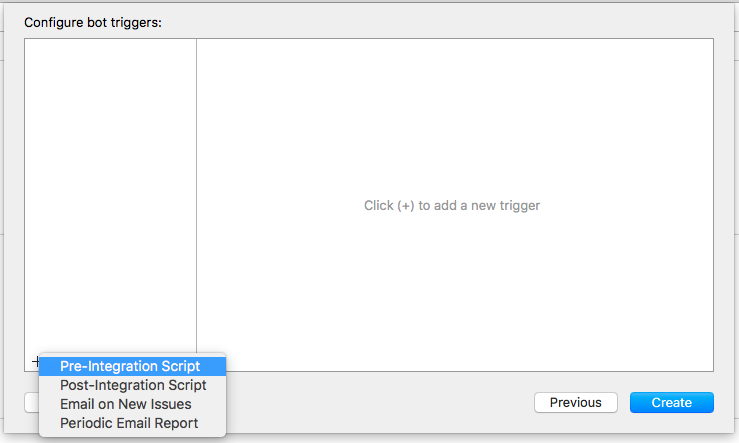
\includegraphics[scale=0.5]{PreIntegrationScript}
\caption{Dodavanje skripte koja se izvršava prije integracije botu}
\label{fig:PreIntegrationScript}
\end{figure}

Unutar novo kreirane skripte je potrebno pozvati sve naredbe koje se trebaju izvršiti prije integracije. Radi jednostavnosti i fleksibilnosti je navedene naredbe korisno izdvojiti u zasebnu datoteku. Korištenjem ovog pristupa olakšavam implementaciju kontinuirane integracije te omogućavam laku izmjenu skripte koja se izvršava prije integracije. Skripta \ref{listing:pre_integration_script_call} se korištenjem \path{XCS_PRIMARY_REPO_DIR} varijable okruženja navigira u početni direktorij projekta te provjerava postojanje datoteke \path{scripts/preintegration}. U slučaju postojanja datoteke ista se izvršava.

\begin{lstlisting}[caption=Poziv skripte koja se izvršava prije integracije, label=listing:pre_integration_script_call]
#!/bin/bash

cd $XCS_PRIMARY_REPO_DIR

if [ -f scripts/preintegration ]; then
    ./scripts/preintegration
fi
\end{lstlisting}

Skripta \ref{listing:pre_integration_script} se izvršava prije integracija. Skripta jednostavno poziva prije definirane skripte. Na isti je način moguće dodati proizvoljan broj naredaba. Dodatno, skripta u \textit{PATH} varijablu okruženja dodaje dvije putanje koje olakšavaju korištenje postojećih alata.

\begin{lstlisting}[caption=Skripta koja se izvršava prije integracije, label=listing:pre_integration_script]
#!/bin/bash

export PATH="/usr/local/bin:~/.gem/ruby/2.0.0/bin/:$PATH"

if [ -f scripts/cocoapods ]; then
    ./scripts/cocoapods
fi

if [ -f scripts/carthage ]; then
    ./scripts/carthage
fi
\end{lstlisting}

Sve skripte se trebaju nalaziti u \path{scripts} direktoriju repozitorija.

\subsection{Izgradnja}

Izgradnja iOS aplikacija se obavlja korištenjem alat \textit{xcodebuild}\citep{xcodebuild}. Alat je razvio Apple za izgradnju programske potpore za macOS operacijski sustav. Alat je vrlo moćan te pruža veliki broj funkcionalnosti i mogućih konfiguracija. Alat je proširen te danas podržava izgradnju aplikacija za iOS, tvOS i watchOS operacijske sustave. Alat izgradnju obavlja na korištenjem Xcode projekta. Prije definiranja procesa izgradnje se je potrebno upoznati sa strukturom Xcode projekta.

Xcode je službeni Appleov alat za razvoj programske potpore za iOS i macOS operacijske sustave. Na tržištu postoji nekoliko alternativa ali je Xcode daleko najkorišteniji. Svi alati koriste alat xocdebuild za izgradnju te zbog toga imaju vrlo sličnu strukturu projekta. Ovaj tip projekta se naziva Xcode projekt.

Xcode projekt sadrži jedan ili više ciljeva \eng{target} i jednu ili više shema \eng{scheme}. Cilj definira postavke koji se koriste kod izvršavanja operacije za navedeni cilj.  Jedan projekt može sadržavati više ciljeva. Pomoću ciljeva je moguće isti kod distribuirati za različite verzije operacijskog sustava, različite operacijske sustave i testirati projekt. Shema definira koji se cilj koristi za koju operaciju. Projekt može koristiti više shema kako bi objedinio operacije za pojedinu distribuciju. Odnos cilja i sheme je prikazan na slici \ref{fig:TargetScheme}. Projekt sadrži tri cilja i dvije sheme. Sheme različito definiraju koji se cilj koristi za koju operaciju.

\begin{figure}[b!]
\centering
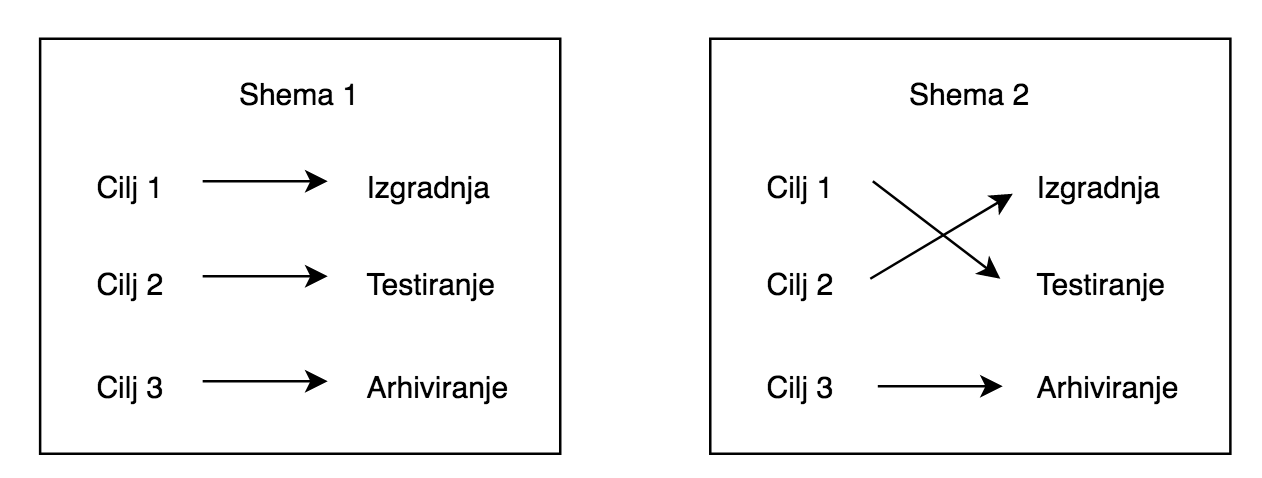
\includegraphics[scale=0.5]{TargetScheme}
\caption{Xcode projekt s tri cilja i dvije sheme}
\label{fig:TargetScheme}
\end{figure}

Xcode projekte je moguće grupirati u Xcode radno okruženje \eng{workspace}. Radno okruženje olakšava segmentiranje velikog projekta i olakšava upravljanje ovisnostima.

Izgradnja iOS projekta se u praksi pokreće gotovo isključivo korištenjem alata Xcode. Međutim, navedeni pristup nije moguće automatizirati. Zbog navedenog procesi koji automatiziraju izgradnju koriste alat xcodebuild, direktno ili korištenjem alata koji interno koristi alat xcodebuild. Alat je detaljnije specificiran u dodatku \ref{header:xcodebuild}.

\begin{figure}
\centering
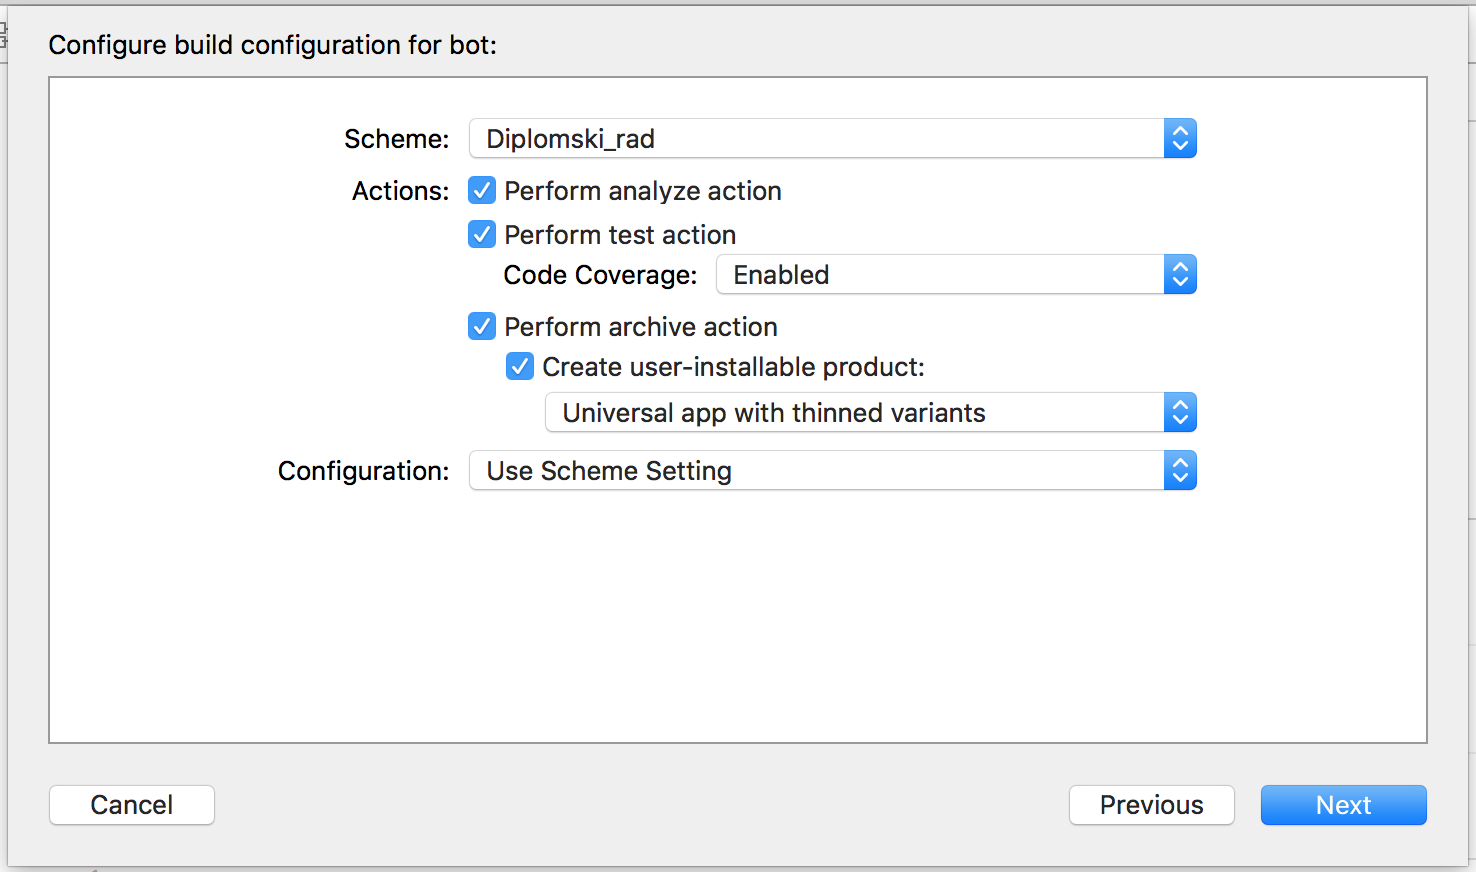
\includegraphics[scale=0.5]{XcodeServerOptions}
\caption{Konfiguracija osnovnih opcija integracije}
\label{fig:XcodeServerOptions}
\end{figure}

\begin{figure}[b!]
\centering
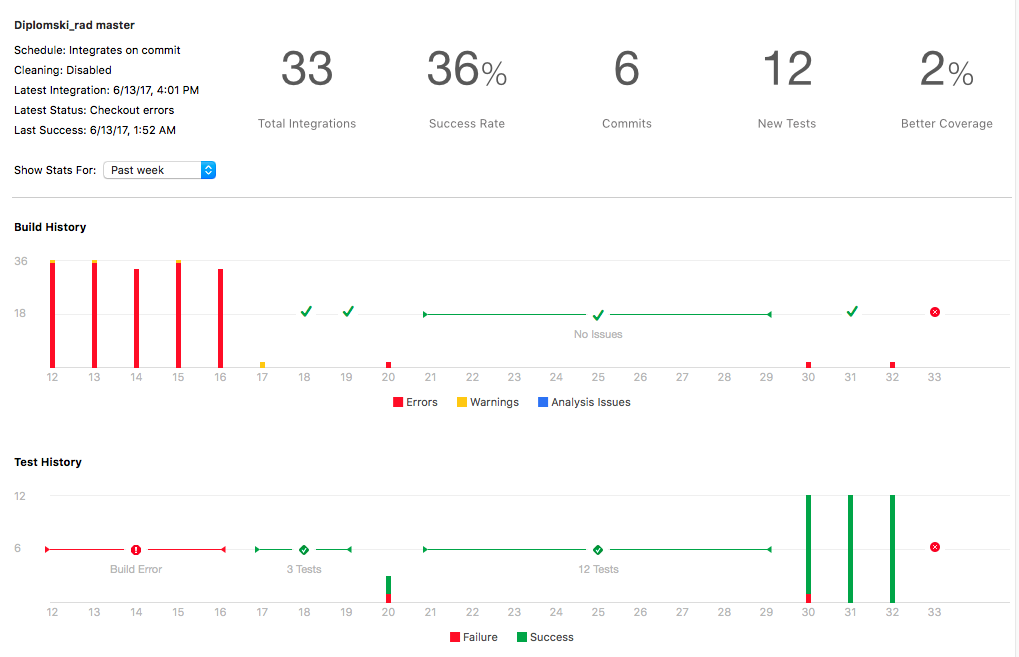
\includegraphics[scale=0.5]{XcodeServerResult}
\caption{Primjer prikaza rezultata kontinuirane integracije}
\label{fig:XcodeServerResult}
\end{figure}

Xcode Server značajno olakšava korištenje alata xcodebuild. Nakon povezivanja bota s repozitorijem izvornog koda je moguće konfigurirati opcije integracije. Moguće je odabrati shemu projekta za koju se provodi integracija, operacije koje će se izvršavati u sklopu integracije te postavke koje se koriste za izgradnju projekta. Slika \ref{fig:XcodeServerOptions} prikazuje opcije koje se mogu konfigurirati.

Kako bi se shema mogla iskoristiti za integraciju ista mora biti javno objavljena. Shema se može konfigurirati korištenjem Xcode aplikacije.

Ovako konfiguriran bot provodi kontinuiranu integraciju za odabranu granu. Rezultat integracije je moguće vidjeti na otvaranjem početnog ekranu bota. Slika \ref{fig:XcodeServerResult} prikazuje primjer rezultata integracije. Prvi redak slike prikazuje opće informacije o kontinuiranoj integraciji kao što broj obavljenih integracija, postotak uspješnosti te broj verzija repozitorija. Drugi redak slike prikazuje uspješnost izvođenja procesa izgradnje za svaku pojedinu integraciju.

Prve dvije prikazane integracije su završile greškom koja je u trećoj integraciji otklonjena. Četvrta integracije otklanja upozorenje dojavljeno u prve tri integracije. Integracija broj 20 dojavljuje novu grešku koju otklanja sljedeća integracija.

Odabirom pojedine integracije se otvara ekran s detaljima odabrane integracije. Detalji integracije su podijeljeni u nekoliko sekcija od kojih svaka pruža vrlo detaljne informacije o integraciji. Prva sekcija \verb|Summary| prikazuje najvažnije podatke na jednom, sažetom ekranu. Slika \ref{fig:XcodeServerSingleIntegration} prikazuje primjer navedene sekcije za integraciju koja je dojavila pet novih pogrešaka u procesu izgradnje. Detalji novo pronađenih pogrešaka su prikazani na ekranu što olakšava pronalaženje i otklanjanje pogrešaka.

\begin{figure}
\centering
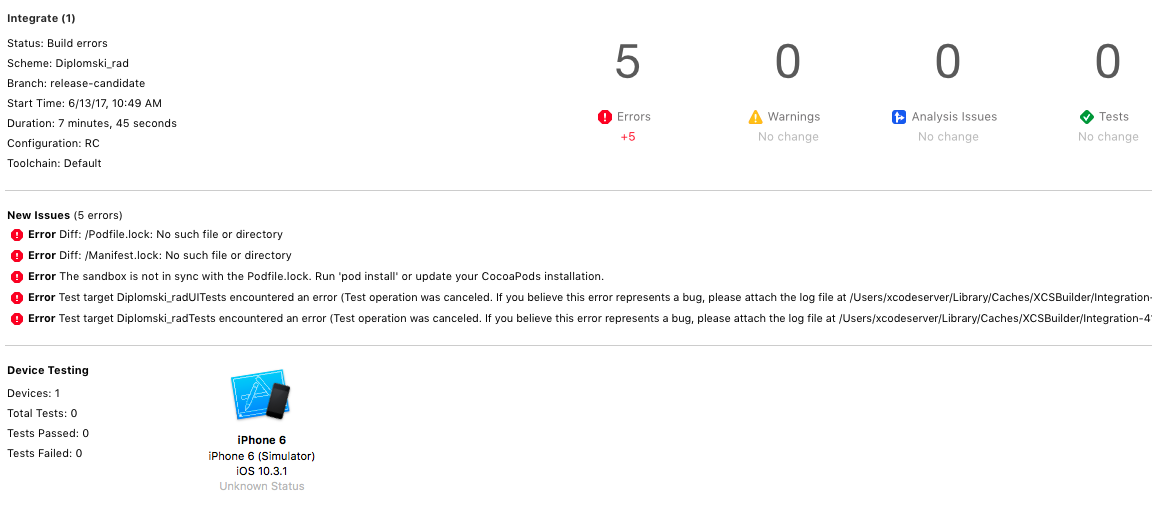
\includegraphics[scale=0.4]{XcodeServerSingleIntegration}
\caption{Detaljan prikaz integracije}
\label{fig:XcodeServerSingleIntegration}
\end{figure}

Zadnja sekcija detaljnog prikaza integracije prikazuje ispis svih faza integracije, uključujući i ručno definirane faze. Sekcija je vrlo korisna za provjeru ponašanja pojedine faze.

\section{Testiranje}

Testiranje je sastavni dio razvoja programske potpore. Implementacijom kvalitetnih testova ne samo da osiguravamo ispravan rad programske potpore, već sprječavamo nazadovanje koda \eng{code regression} i značajno smanjujemo potrebu za ručnim testiranjem ispravnosti\citep{wiki:SoftwareTesting}.

Pogrešno je mišljenje da implementacija testova produljuje vrijeme razvoja. Svaku implementiranu funkcionalnosti i obavljenu izmjenu je potrebno testirati. Jedino je pitanje hoće li se navedeno testiranje obavljati automatski. Jednom napisan kvalitetan test se može pokrenuti proizvoljan broj puta. S druge strane, provođenje ručanog testiranje svaki put zahtijeva vrijeme člana tima. Bilo to u sklopu razvoja ili s ciljem provjere ispravnosti, ručna provjera ispravnosti zahtjeva više resursa i daje lošije rezultate.

Navedenu konstataciju ne treba zamijeniti s potpunim isključenjem ručnog testiranja aplikacije. Bez obzira na kvalitetu testova pogreške se uvijek mogu dogoditi. Međutim, pisanjem kvalitetnih testova se vjerojatnost pojave pogreške značajno smanjuje.

Ovaj odlomak ne ulazi u proces pisanja testova, već samo automatizira pokretanje istih. Implementacija kvalitetnih testova je vrlo složeno područje te nadilazi okvire ovog rada.

Proces razvoja programske potpore za iOS operacijski sustav definira dva tipa testova: \verb|unit| i \verb|UI| testove.

Unit testovi su nesretno imenovani. Oni ne predstavljaju standardne unit testove, već se koriste kao ime za testove koji imaju pristup kodu koji testiraju. Testovi direktno komuniciraju s kodom koji testiraju i kroz ovu komunikaciju provjeravaju ispravnost izvođenja. Ovaj tip testa se pokreće kao omotač oko izvorne aplikacije.

S druge strane, UI testovi nemaju pristup izvornom kodu aplikacije. Oni programsku potporu testiraju njezinim pokretanjem i simuliranjem korisničke interakcije. Programer specificira korisničke akcije i ponašanje koje očekuje od aplikacije nakon primanja navede akcije. UI testovi pokreću dvije aplikacije: aplikaciju koju testiraju i aplikaciju koja simulira korisničku interakciju.

Oba tipa testova su implementirani kao testni ciljevi Xcode projekta. Kod testnog cilja nije dio produkcijskog te se ne koristi u procesu izgradnje. Testni cilj referencira cilj koji testira. Dodatno, shema može specificirati koji se testni ciljevi pokreću prilikom pokretanja operacije testiranja. Na ovaj način jedna shema može u procesu testiranja pokrenuti više testnih ciljeva.

Proces testiranja se može pokrenuti na iOS Simulatoru, aplikaciji koja simulira iOS operacijski sustav na macOS operacijskom sustavu, ili stvarnom uređaju. Simulator se instalira u sklopu instalacije Xcode aplikacije.

\subsection{Automatizacija testiranja}

\begin{figure}[b!]
\centering
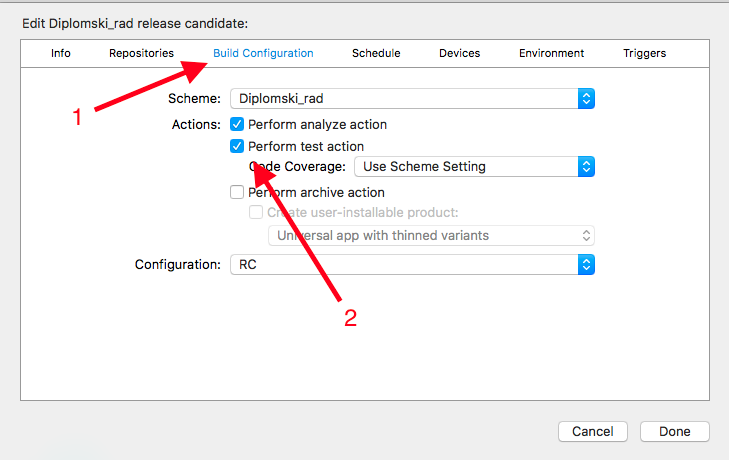
\includegraphics[scale=0.5]{XcodeServerTestAction}
\caption{Uključivanje pokretanja testova u sklopu integracije}
\label{fig:XcodeServerTestAction}
\end{figure}

\begin{figure}
\centering
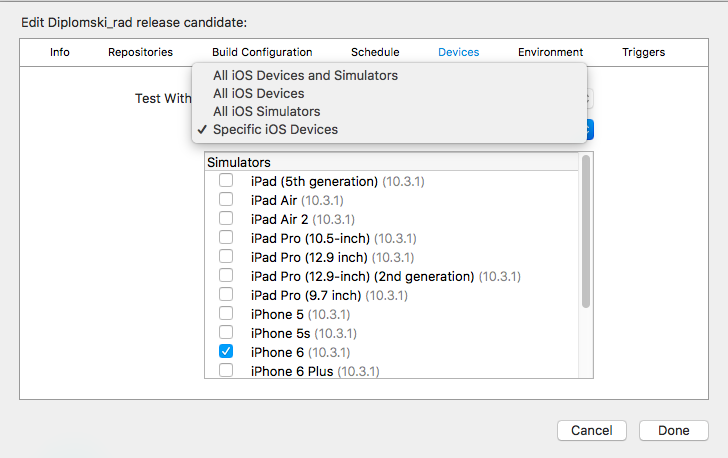
\includegraphics[scale=0.5]{XcodeServerTestDevices}
\caption{Odabir uređaja na kojima se pokreću testovi}
\label{fig:XcodeServerTestDevices}
\end{figure}

Xcode Server detektira testne ciljeve sheme za koju obavlja proces integracije. Za pokretanje testova u sklopu integracije odabrati opciju \verb|Edit bot...| te u sekciji \verb|Build configuration| označiti opciju \verb|Perform test action|. Slika \ref{fig:XcodeServerTestAction} prikazuje navedeni proces. Sljedeća obavljena integracija će pokrenuti sve testne ciljeve koje definira odabrana shema.

Dodatno, moguće je odabrati uređaje na kojima se pokreću testovi. Testove je moguće pokrenuti na svim dostupnim uređajima, samo na dostupnim iOS simulatorima, samo na dostupnim stvarnim uređajima ili na samo odabranim uređajima. Slika \ref{fig:XcodeServerTestDevices} prikazuje navedeni izbornik. Izborniku se pristupa odabirom opcije \verb|Edit bot...| te otvaranjem sekcije \verb|Devices|.

Novi testni cilj je shemi moguće dodati korištenjem Xcode aplikacije. Pokrenuti iOS projekt te odabrati željenu shemu iz padajućeg izbornika u gornjoj alatnoj traci aplikacije. Odabirom opcije \verb|Edit scheme| se otvara prozor prikazan na slici. U lijevom izborniku odabrati opciju \verb|Test| te pritiskom na plus ikonu dodati željeni testni cilj postojećoj shemi. Nakon spremanja promjene integracija u sljedećem izvršavanju obavlja i novo dodani testni cilj.

\begin{figure}[b!]
\centering
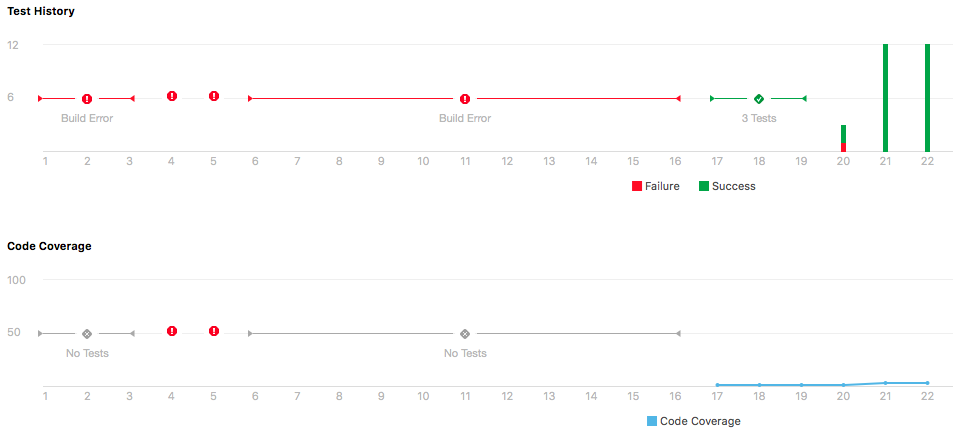
\includegraphics[scale=0.4]{XcodeServerTestResult}
\caption{Rezultati procesa testiranja i osiguranja kvalitete}
\label{fig:XcodeServerTestResult}
\end{figure}

Rezultati obavljanja testova su također na početnom ekranu bota u sekciji \verb|Test History|. Osim broja uspješnih i neuspješnih testova, alat omogućuje i prikaz detaljnih rezultata testiranja. Odabirom rezultata testiranja pojedine integracije se prikazuju detalji odabranog testiranja.


\section{Osiguranje kvalitete}

Osiguranje kvalitete \eng{code quality} je proces u sklopu programskog inženjerstva koje postavljanjem umjetnih restrikcija nastoji poboljšati kvalitetu koda i konačnog produkta. Restrikcije se najčešće definiraju u obliku pravila koja moraju biti zadovoljena. Pravila se mogu kretati od jednostavnih do vrlo složenih te uvelike ovise o korištenim alatima i potrebama tima.

U sklopu rada implementiram dvije provjere: provjeru pokrivenosti koda testovima i provjeru ispravnosti koda korištenjem alata Swiftlint.

Pokrivenost koda testovima \eng{code coverage} je mjera koja govori u kolikom je postotku izvorni kod pokriven testovima. Svaki redak koda koji je barem jednom izvršen u procesu testiranja je pokriven testovima. Što je navedena mjera veća to je više koda testirano. Zbog toga možemo reći da veća pokrivenost koda testovima, u generalnom slučaju, vodi k boljoj kvaliteti konačnog produkta.

Međutim, navedena se mjera može vrlo lako zloupotrijebiti. Na primjer, moguće je napisati vrlo jednostavan test koji samo pokreće aplikaciju i time poziva značajan postotak koda. Zbog navedenog se u praksi često koriste modificirane verzije mjerenja pokrivenosti koda testovima koje procesu dodaju dodatna pravila te time nastoje utvrditi stvarnu kvalitetu testiranja\citep{wiki:CodeCoverage}.

Alat xcodebuild implementira mjerenje pokrivenosti koda testovima. Dovoljno je naredbi za pokretanje testova dodati argument \verb|-showBuildSettings|. Ispis naredbe se pohranjuje kao skup datoteka koje služe za vizualan prikaz pokrivenosti koda testovima u Xcode aplikaciji. Uz sam postotak pokrivenosti koda testovima, Xcode prikazuje i pokrivenost pojedinog dokumenta te broj poziva svake pojedine linije koda.

Xcode Server omogućava prikupljanje podataka o pokrivenosti koda testovima u sklopu integracije projekta. Prikupljanje podatka o pokrivenosti koda testovima se uključuje odabirom opcije \verb|Code Coverage -> Enabled| u postavkama bota. Slično Xcode aplikaciji, Xcode Server uz postotak pokrivenosti koda testovima prikazuje i pokrivenost pojedinog dokumenta. Slika \ref{fig:XcodeServerTestCoverage} prikazuje pokrivenost datoteka testnog projekta testovima. Međutim, vrlo je teško automatizirati provjeru pokrivenosti koda testovima. Trenutno ne postoji mogućnost dohvata podataka prikazanih na slici izvan alata Xcode Server. Zbog navedenog provjeru pokrivenosti koda testovima obavljam ručno.

\begin{figure}[h!]
\centering
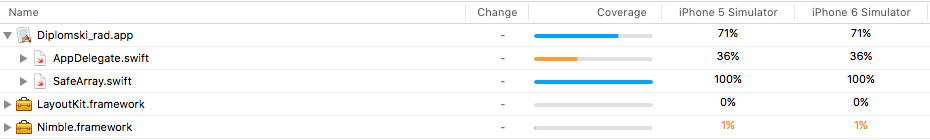
\includegraphics[scale=0.45]{XcodeServerTestCoverage}
\caption{Pokrivenost datoteka testnog projekta testovima}
\label{fig:XcodeServerTestCoverage}
\end{figure}

Swiftlint je alat za statičku analizu koda napisanog u programskom jeziku Swift. Alat definira veliki broj pravila kojima nastoji osigurati praćenje stila i konvencija jezika Swift\citep{SwiftLint}. Većina pravila se odnosi na izgled i format koda, ali postoje i pravila koja nastoje izbjeći pojavu grešaka. Slični alati su kreirani za gotovo svaki programski jezik koji se koristi u praksi. Ovi alati se nazivaju alati za uređivanje koda \eng{linting tools}. Navedene alate uglavnom kreira i održava zajednica.

Ne poštivanje pravila izaziva dojavu upozorenja \eng{warning} ili greške \eng{error}. Moguće je kreirati nova pravila i modificirati ili isključiti postojeća. Veliki broj timova definira vlastiti stil pisanja koda koji je moguće osigurati korištenjem navedenih funkcionalnosti.

Alati za uređivanje koda postaju nezaobilazni u praksi. Pridržavanje strogog formata pisanja koda olakšava timski rad, poboljšava čitljivost koda i izbjegava pojavu lako izbjegnutih grešaka.

Alat se pokreće pozivom naredbe \path{swiftlint} u početnom direktoriju projekta. Naredbu je moguće ukljućiti u proces izgradnje korištenjem \verb|Run Script| faze. Pomoću Xcode aplikacije otvoriti željeni projekt te odabrati cilj koji izvršava izgradnju. U sekciji \verb|Build Phases| odabirom opcije \verb|Plus -> New Run Script Faze| kreirati novu fazu. Fazi dodati sadržaj skripte \ref{listing:swiftlint}.

\begin{lstlisting}[caption=Provjera postojanja i pokretanje Swiftlint alata, label=listing:swiftlint]
if which swiftlint >/dev/null; then
    swiftlint
else
    echo "warning: Swiftlint nije instaliran"
fi
\end{lstlisting}

Ako je poziv \path{swiftlint} naredbe dodan kao faza izgradnje, onda se naredba obavlja prilikom svake izgradnje. Ispis naredbe se parsira zajedno s ispisom xcodebuild alata te se rezultati dojavljuju zajedno. Ako naredba nije dodana projektu onda je poziv potrebno ručno implementirati nakon obavljanja integracije.


\chapter{Kontinuirana dostava}

Kontinuirana dostava je praksa u sklopu programskog inženjerstva koja automatiziranjem procesa isporuke programske podrške nastoji olaškati i time povećati učestalost isporuke produkta u produkciju. Proces isporuke može biti kompleksan i vremenski zahtjevan. Prije isporuke je produkt potrebno izgraditi, testitirati, kreirati artefakt koji se isporučuje te ga objaviti na željenoj platformi. Za izgradnju je potrebno dohvatiti željenu verziju repozitorija, pripremiti sustav te dohvatiti sve potrebne ovisnosti.

Navedeni proces je vremenski zahtjevan zbog čega se on ne provodi često. Rijetko provođenje procesa isporuke uzrokuje nekoliko problema. Prvo, rijetkom isporukom se veći broj funkcionalnosti grupira i isporučuje zajedno. Što je veći broj funkcionalnosti isporučen zajedno i što duže te funkcionalnosti nisu isporučene, to je teže osigurati ispravnost isporučenih funkcionalnosti. Dodatno, što duže funkcionalnost nije objavljena to je veći propušteni dobitak koji je funkcionalnost mogla donjeti. Svaka funkcionalnost se razvija s određenim ciljem. Nakon što je funkcionalnost razvijena a prije nego što je objavljena navedeni cilj ostaje bespotrebno ne ispunjen.

Automatizacija procesa isporuke značajno olakšava navedeni proces i time potiče češću isporuku. Dodatno, implementacija jednostavnog i automatiziranog procesa isporuke smanjuje mogućnost pojave ljudske pogreške. Kontinuirana dostava na navedeni naćin nastoji smanjiti trošak, rizik i vrijeme razvoja programske potpore te isto vrijeme poboljšati kvalitetu i osigurati ispravnost programskog produkta\citep{wiki:ContinuousDelivery}.

Kao što je navedeno u uvodu poglavlja, programsku potporu je prije isporuke potrebno izgraditi, testirati te kreirati artefakt za isporuku. Iako različiti razvojni procesi različito nazivaju artefakt za distribuciju, zbog konzistentnosti ga nazivam arhiva. Arhiviranje je proces kreiranje arhive programske potpore. Arhiva omogućava instalaciju programske potpore na operacijskom sustavu za kojeg je programska potpora izgrađena.

Jednako tako je prije automatizacije isporuke produkta potrebno automatizirati izgradnju, testiranje, provjeru ispravnosti i arhiviranje programske potpore. Proces automatizacije izgradnje, testiranja i provjere ispravnosti se naziva kontinuirana integracija te je definiran u poglavlju \ref{header:Kontinuirana_Integracija}. Kontinuirana dostava obuhvaća proces kontinuirane integracije te proces automatizacije isporuke.

Međutim, u praksi se pojam kontinuirana dostava češće koristi za proces automatizacije isporuke koji zahtijeva odvojenu implementaciju procesa kontinuirane integracije. Zbog jednostavnosti se navedeni pristup koristi u ovom radu. Proces izgradnje, testiranja i provjere ispravnosti implementiram u sklopu kontinuirane integracije na koju dodajem automatizaciju isporuke i time ostvarujem kontinuiranu dostavu.

Važno je napomenuti da kontinuirana dostava ne isporučuje produkt automatski, već samo automatizira proces isporuke. Tim još uvijek mora pokrenuti proces isporuke za željenu verziju produkta. Automatska objava programske potpore je obrađena u sljedećem, \ref{header:KontinuiranaIsporuka} poglavlju.

Programsku potporu je moguće isporučiti na više načina - direktnom instalacijom na mobilni uređaj, ručnom distribucijom arhive, objavom arhiva korištenjem distribucijske platforme ili objavom arhive koriptenjem App Store platforme. Navedeni tipovi isporuke dijele sličan proces izgradnje i arhiviranja ali se značajno razlikuju u procesu objave arhive. Samim time se i automatizacije navedenih načina isporuke značajno razlikuju.

iOS operacijski sustav podržava četiri tipa isporuke: direktnu isporuku \eng{direct distribution}, \textit{ad hoc} isporuku \eng{ad hoc distribution}, unutarnju isporuku \eng{in-house distribution} i isporuku korištenjem App Store platforme. Odabir načina isporuke ovisi o korisnicima za koje se obavlja isporuka.

Direktna isporuka progrmsku potporu instalira direktno na povezani mobilni uređaj. Mobilni uređaj mora biti povezan s računalom koje obavlja isporuku te mora biti registriran kao testni uređaj na Apple Developer platformi. Ovaj tip isporuke programsku potporu instalira na jedan uređaj koji mora biti direktno povezan s računalom zbog čega se koristi gotovo isključivo u sklopu razvoja i za isporuku programske potpore unutar razvojnog tima. Dodatno, ovaj se tip isporuke se nemože niti bi ga bilo pogodno automatizirati. Zbog sigurnosnih razloga Apple nije objavio proces direktne isporuke već ju je moguće obaviti isključivo korištenjem Xcode aplikacije.

Ad hoc i unutarnja isporuka su vrlo slične. Obje proizvode arhivu koju je potrebno samostalno dostaviti željenim korisnicima. Arhiva se može dostaviti ručno, na primjer korištenjem e-mail poruke ili se može objaviti na platformi za distribuciju programske potpore. Moguće je kreirati vlastitu platformu ili iskoristiti neku velikog broja već postojećih. Isporuke se razlikuju u tome što uređaji na koje se instalira programska potpora isporučena ad hoc načinom isporuke moraju biti registrirani kao testni uređaju na Apple Developer platformi dok to nije potrebno za unutanju isporuku. Zbog navedenog je korištenjem unutranje isporuke programsku potporu moguće isporučiti neograničenom broju korisnika. Za korištenje unutarnje isporuke je potrebno posjedovati \textit{Enterprise} Apple Developer račun, skuplju verziju običnog Apple Developer računa.

Ad hoc isporuka se najčešće koristi za isporuku programske potpore unutar tima, na primjer za isporuku testne verzije aplikacije timu za osiguranje kvalitete. Unutarnja isporuka se koristi gotovo isključivo za isporuku aplikacija razvijenih za unutarnje potrebe kompanije. Ovaj tip isporuke se nesmije iskoristiti za objavu aplikacija namijenjenih za javno tržište.

App Store isporuka se koristi za objavu programske potpore namijenjene za javno tržište. Za razliku od ostalih tipova isporuke, Apple strogo nadzire aplikacije objavljene ovim tipom isporuke. Svaka aplikacija koja zatraži objavu prolazi kroz strog proces provjere kvalitete i podudaranja s velikim brojem Appleovih smjernica. Ovaj proces može trajati i nekoliko tjedana zbog čega je nužno osigurati ispravnost aplikacije prije pokretanja procesa. Svaka izmjena aplikacije prolazi nešto kroz kraći proces provjere koji može trajati od nekoliko sati do nekoliko dana.

Iako se navedeni tipovi isporuke razlikuju u implementaciji, moguće ih je generalno podijeliti u tri ista koraka: potpisivanja koda, arhiviranja programske potpore i objave arhive. Svaki od koraka je definiran i automatiziran odvojeno u nastavku poglavlja. Slika \ref{fig:ContinuousDelivery} prikazuje navedenu podjelu.

\begin{figure}
\centering
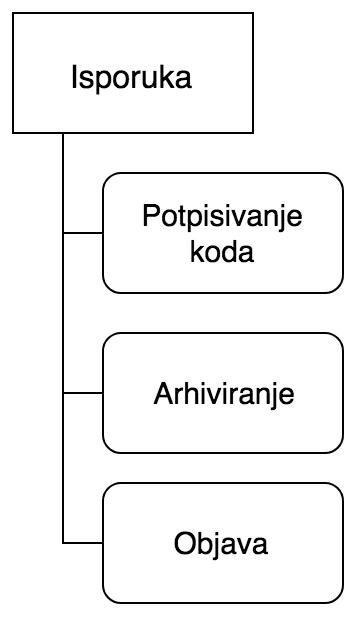
\includegraphics[scale=0.6]{ContinuousDelivery}
\caption{Proces isporuke}
\label{fig:ContinuousDelivery}
\end{figure}

\section{Potpisivanje koda} \label{header:PotpisivanjeKoda}

Kako bi osigurao autentičnost i neizmjenjenost programske potpore, iOS operacijski sustav implementira proces potpisivanja koda \eng{code signing}. Proces korištenjem certifikata, identifikatora aplikacije \eng{application identificator} i pripremnih profila \eng{provisioning profiles} potpisuje i enkriptira kreiranu arhivu. Prije kreiranja arhive je potrebno kreirati i dohvatiti navedene artefakte te ispravno konfigurirati proces arhiviranja.

Proces postpisivanja koda se može podijeliti na tri faze: kreiranje artefakata, dohvat artefakata i konfiguracija procesa arhiviranja. Slika \ref{fig:CodeSigning} prikazuje navedenu podjelu.

\begin{figure}
\centering
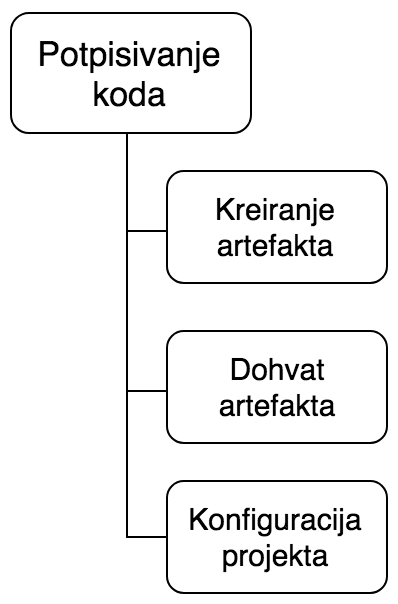
\includegraphics[scale=0.6]{CodeSigning}
\caption{Potpisivanje koda}
\label{fig:CodeSigning}
\end{figure}

Ako potrebni artefakti ne postoje iste je potrebno kreirati te nakon toga preuzeti i instalirati na računalu. Proces arhiviranja je zatim potrebno konfigurirati kako bi koristio ispravne artefakte.

Svi artefakti se kreiraju i dohvaćaju korištenjem \path|https://developer.apple.com| platforme. Potrebno se je prijaviti na platformu korištenjem Apple Developer računa, odabrati opciju \verb|Certificates, Identifiers & Profiles| i željeni tip artefakta iz lijevog bočnog izbornika.

Certifikati se koriste za osiguranje nekoliko različitih procesa zbog čega postoji nekoliko tipova certifikata. U sklopu isporuke nas zanimaju dva tipa certifikata: razvojni \eng{development} i produkcijski \eng{production} certifikati. Razvojni certifikati se koriste u razvoju i za direktnu isporuku programske potpore. Uobičajno je kreirati zaseban certifikat za svakog člana tima. Produkcijski certifikati se koriste za ad hoc, unutarnju i App Store isporuku. Standardno je kreirati jedan certifikat po timu koji obavlja isporuku. Certifikat se kreira pomoću \verb|CSR| datoteke koju je moguće kreirati korištenjem Keychain Access aplikacije.

Pokrenuti Keychain Access aplikaciju te u izborniku na vrhu ekrana odabrati opciju \verb|Certificate Assistant -> Request a Certificate|. U novo otvorenom prozoru unijeti e-mail adresu Apple Developer računa, odabrati \verb|Save to disk| opciju i lokaciju spremanja novo kreirane datoteke. Kreiranu datoteku dostaviti u formu za kreiranje certifikate na Apple Developer platformi te nakon toga obrisati datoteku.

Za korištenje certifikata je potrebno posjedovati certifikat i privatni ključ kojim je on kreiran. Certifikat je moguće preuzeti s Apple Developer platforme dok je privatni ključ potrebno dohvatiti s računala koje posjeduje privatan ključ. Nakon kreiranja certifikata to je isključivo uređaj koji je kreirao CSR datoteku. Za dohvat privatnog ključa pokrenuti Keychain Access aplikaciju te pronaći željeni certifikat. Ako na uređaju postoji privatni ključ navedenog certifikata, isti je moguće izdvojiti korištenjem opcije \textit{Export}. Slika \ref{fig:PrivateKeyExport} prikazuje izdvajanje privatnog ključa certifikata.

\begin{figure}
\centering
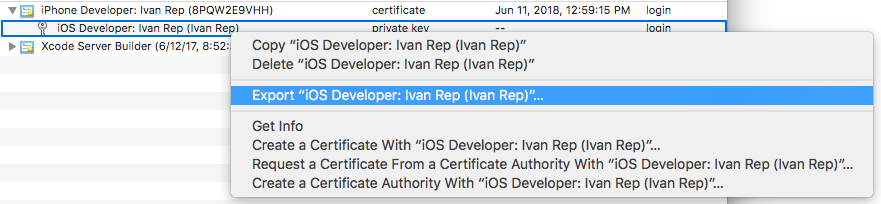
\includegraphics[scale=0.47]{PrivateKeyExport}
\caption{Izdvajanje privatnog ključa certifikata}
\label{fig:PrivateKeyExport}
\end{figure}

Ovako izdvojeni privatni ključ certifikata je moguće distribuirati. Nužno je osigurati tajnost privatnog ključa jer suprotno narušava sigurnost svih aplikacija koje koriste navedeni certifikat.

Identifikator aplikacije identificira i opisuje servise koje koristi aplikacija koja se isporučuje. Identifikator aplikacije je definiran pomoću identifikatora paketa \eng{bundle identifier}, niza znakova jedinstvenog za svaku aplikaciju. Identifikator paketa je najčešće oblika \path{com.ime_kompanije.ime_aplikacije}. Postoje dva tipa identifikatora aplikacije: \textit{wildcard} i eksplicitni identifikatori aplikacije. Wildcard identifikatori aplikacije specificiraju samo dio identifikatora paketa te ih karakterizira asterisk (*) u sklopu imena, na primjer \path{com.rep.*}. Sve aplikacije čiji identifikator paketa započinje navedenim nizom znakova mogu biti isporućene korištenjem navedenog identifikatora. Wildcard identifikatori se koriste u razvoju programske potpore. Eksplicitni identifikatori jedinstveno identificiraju aplikaciju, na primjer \path{com.rep.testna_aplikacija} te se koriste za isporuku specifične aplikacije.

Za kreiranja identifikatra aplikacija je potrebno specificirati ime identifikatora, dodati identifikator paketa i odabrati servise koje aplikacija koristi. Nakon kreiranja je identifikator potrebno preuzeti i pokrenuti korištenjem Keychain Access aplikacije.

Pripremni profil povezuje identifikator aplikacije i certifikat. Svaki od četiri tipa isporuke definira vlastiti tip pripremnog profila. Kreiranje pripremnog profila započinje odabirom tipa profila i odabirom odgovarajućeg identifikatora aplikacije i certifikata. Pripremni profil za direktnu isporuku zahtijeva razvojni certifikat, dok pripremni profili ostalih tipova isporuka zahtijevaju produkcijski certifikat.

\begin{figure}
\centering
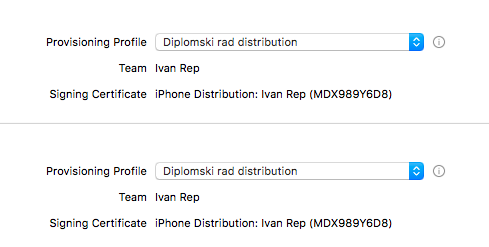
\includegraphics[scale=0.6]{SigningArtefactsSetup}
\caption{Postavljanje artefakta za potpisivanje koda}
\label{fig:SigningArtefactsSetup}
\end{figure}

Novo kreirana artefakte je potrebno preuzeti i pripremiti za korištenje. Profile je potrebno spremiti na računalu koje obavlja isporuku u direktoriju \path|~/Library/MobileDevice/Provisioning Profiles/| a certifikate je potrebno pokrenuti korištenjem Keychain Access aplikacije.

Prije pokretanja arhiviranja je potrebno konfigurirati projekt kako bi se u sklopu arhiviranja koristili ispravni artefakti. Otvoriti Xcode projekt, odabrati željen cilj u sekciji \textit{General} podstaviti \textit{Debug} i \textit{Release} certifikate za potpisivanje koda.

\begin{figure}[b!]
\centering
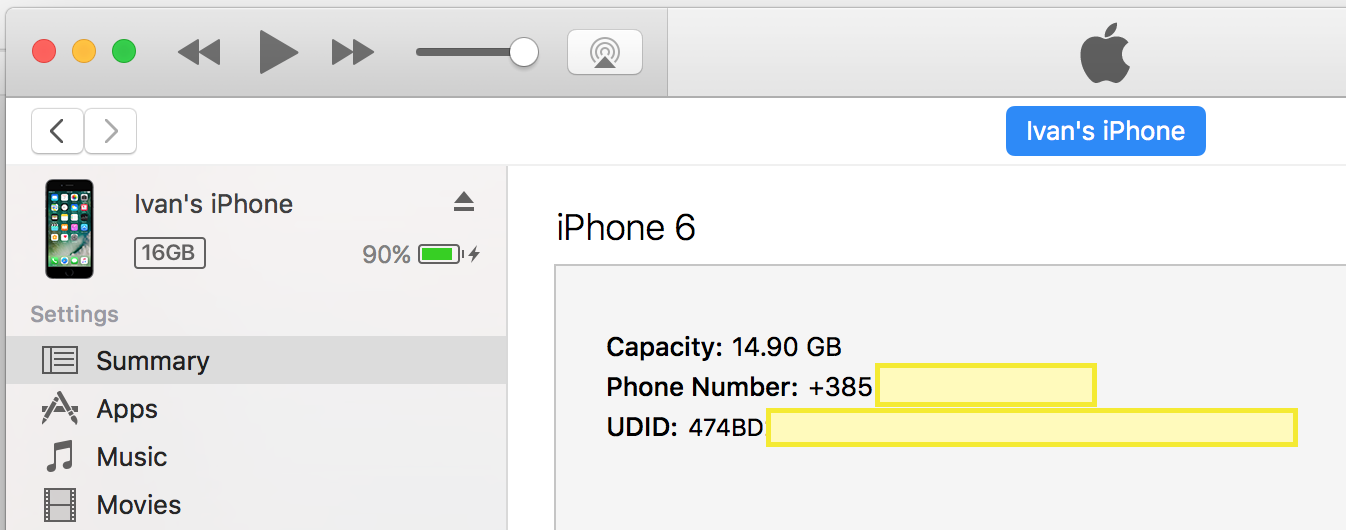
\includegraphics[scale=0.5]{iTunesUUID}
\caption{Dohvat UUIDa uređaja korištenjem iTunes aplikacije}
\label{fig:iTunesUUID}
\end{figure}

Direktna i ad hoc isporuka zahtijevaju registraciju mobilnog uređaja kao testnog uređaja korištenjem Apple Developer platforme. Uređaj se registrira korištenjem njegovog UUID identifikatora. UUID se može dohvatiti korištenjem iTunes aplikacije dostupne u sklopu instalacije macOS operacijskom sustavu. Potrebno je povezati mobilni uređaj s računalom korištenjem USB kabela te u iTunes aplikaciji odabrati povezani mobilni uređaj i kopirati njegov UUID. Slika \ref{fig:iTunesUUID} prikazuje lokaciju UUID broja u iTunes aplikacije.

\subsection{Automatizacija potpisivanja koda}

Ručno kreiranje i održavanje certifikati i profila se može vrlo lako zakomplicirati. Ne samo da je proces kreiranja sam po sebi složen, već je potrebno i ispravno distribuirati artefakte bez ugrožavanja njihove sigurnosti. Artefakte se mogu slobodno distribuirati, ali je njihove privatne ključeve nužno održati tajnim. Do prije nekoliko godina se je cijeli proces odrađivao ručno. Nakon kreiranja artefakata isti su se zajedno s privatnim ključem pohranili na sigurnu lokaciju te distribuirali po potrebi.

Danas na tržištu postoji nekoliko pristupa i alata koji olakšavaju i automatiziraju proces potpisivanja koda. Automatizacija potpisivanja koda se oslanjaju na javan API Apple Developer platforme koji omogućuje kreiranje, modificiranje i dohvat svih artefakata navedenih u prošlom odlomku.

Dodatno, večina alata se zalaže za pohranu artefakata zajedno s pripadajučim privatnim ključevima u jednom tajnom git repozitoriju. Na ovaj se način njihova pohrana i dohvat značajno pojednostavljuju te je cijeli proces moguće jednostavno automatizirati. Međutim, pohrana sigurnosnih podataka u git repozitoriju donosi i određeni sigurnosni rizik. Pristup repozitoriju je nužno detaljno nadzirati. Preporuća se SSH protokol definirana u \ref{header:Verzioniranje} odlomku. Dodatno, korisno je repozitorij pokrenuti unutar lokalne mreže kako on ne bi bio vidljiv izvan mreže\citep{codesigningguide}.

Automatizaciju potpisivanja koda u ovom radu ostvarujem korištenjem alata \verb|match| koji je dio \verb|fastlane| familije\citep{fastlane:match}. Alat samostalno kreira, dohvaća i priprema potrebne artefakte i time značajno olakšava proces potpisivanja koda.

Alat match se inicijalizira pozivanjem naredbe \verb|fastlane match init| u početnom direktoriju projekta. Proces inicijalizacije zahtijeva unos lokacije git repozitorija te autorizaciju pristupa repoztoriju. Lokacija repozitorija se zajedno s ostalim parametrima alata sprema u \verb|Matchfile| datoteku gdje je iste moguće modificirati..

Match radi povećanja sigurnosti zahtjeva da SSH ključ korišten u procesu SSH autentifikacije bude vidljiv samo trenutnom korisniku operacijskog sustava. Skripta \ref{listing:ssh_chmod} modificira prava pristupa za odabrani ključ kako bi njegovo korištenje bilo dostupno samo trenutnom korisničkom računu operacijskog sustava.

\begin{lstlisting}[caption=Ograničavanje prava pristupa SSH ključu na samo trenutnog korisnika, label=listing:ssh_chmod]
chmod 600 ~/.ssh/{imekljuca}.pub
\end{lstlisting}

Dodatno, potrebno je konfigurirati SSH protokol kako bi isti koristi željeni ključ. Kreirati novu datoteku \path|.ssh/config| sa sadržajem skripte \ref{listing:SSH_match}.

\begin{lstlisting}[caption=Postavke SSH protokola za alat match, label=listing:SSH_match]
Host *
UseKeychain yes
AddKeysToAgent yes
IdentityFile ~/.ssh/{imekljuca}
\end{lstlisting}

Alata match sve potrebne certifikate i profile kreira i dohvaća automatski. Dovoljno je pokrenuti alat i specificirati tip isporuke koji se koristi. Alat definira četiri tipa koji odgovaraju prethodno definiranim tipovima isporuke: \verb|development|, \verb|adhoc|, \verb|enterprise| i \verb|appstore|. Naredba u nastavku dohvaća i po potrebi kreira artefakte za ad hoc isporuku.

\begin{lstlisting}[caption=Dohvćanje artefakta pomoću dodatka match za ad hoc isporuku]
match(type: 'adhoc')
\end{lstlisting}

Alat ne obavlja konfiguraciju procesa arhiviranja, međutim, budući da je istu potrebno napraviti samo jednom ona se najčešće obavlja ručno. Pomoću match alata kreirati sve potrebne artefakte odnosno pozvati match naredbe za svaki tip isporuke koja se koristi. Navedene će naredbe kreirati i dohvatiti potrebne artefakte. Zatim otvoriti Xcode aplikaciju i odabrati željenu shemu. Na početnoj, \verb|General| sekciji sheme u odlomku \verb|Signing| za svaku konfiguraciju postaviti odgovarajući pripremni profil.

Nakon spremanja promjena se cijeli proces potpisivanja koda svodi na poziv alata match sa željenim tipom isporuke.


\section{Arhiviranje} \label{header:RucnaIsporuka}

Arhiviranje je proces kreiranja artefakta pomoću kojeg se aplikacija instalira na korisničkom uređaju. Artefakt se naziva arhiva aplikacije te je označena \verb|.ipa| nastavkom. Za instalaciju aplikacije je uz arhivu potrebna i datoteka koja opisuje, verificira i locira arhivu. Navedena se datoteka naziva manifest te je označena \verb|.plist| nastavkom.

Proces arhiviranja se za ad hoc, unutarnju isporuku i App Store ispruku razlikuje jedino u odabiru tipa isporuke. Arhiviranje obavlja alat xcodebuild. Međutim, alat je vrlo složen i pruža veliki broj opcija zbog čega na tržištu postoji nekoliko alata koji olakšavanju njegovo korištenje. U sklopu rada za ručno arhiviranje koristim aplikaciju Xcode a za automatizirano arhiviranje alat fastlane odnosno njegov dodatak \verb|gym|. Proces arhiviranja korištenjem alata xcodebuild je prikazan u dodatku \ref{header:xcodebuild}.

Korištenjem aplikacije Xcode odabrati opciju \verb|Product -> Archive| iz izbornika na vrhu ekrana. Nakon kračeg perioda se otvara novi prozor koji prikazuje sve dosad kreirane arhive. Jedino što je potrebno je arhivu izdvojiti za objavu. U prozoru odabrati opciju \verb|Export...|. Otvara se novi prozor u kojem je potrebno odabrati željeni tip isporuke te odabrati između nekoliko opcija kreiranja arhive. Slika \ref{fig:XcodeArchiveOptions} prikazuje početni ekran prozora odnosno odabir tipa isporuke arhive. Nakon odabira željene opcije slijediti upute za dovršenje izdvajanja arhive.

\begin{figure}
\centering
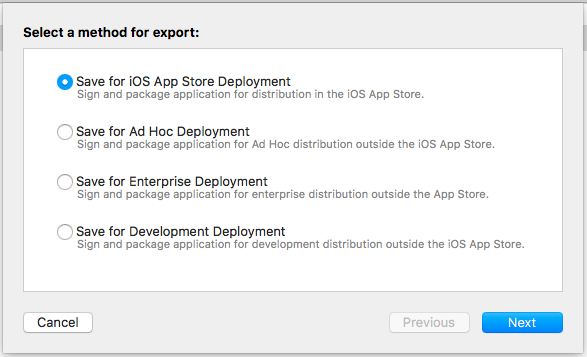
\includegraphics[scale=0.6]{XcodeArchiveOptions}
\caption{Odabir tipa isporuke u procesu kreiranja arhive}
\label{fig:XcodeArchiveOptions}
\end{figure}

Proces generira dvije datoteke prethodno definirane datoteke. Arhivu aplikacije s \verb|.ipa| nastavkom i manifest aplikacije s \verb|.plist| nastavkom.

Direktna isporuka aplikaciju instalira na mobilni uređaj koji je direktno povezan s računalom koje obavlja isporuku. Zbog navedenog proces arhiviranja u sklopu direktne isporuke ne rezultira arhivom već istu direktno instalira na uređaj. Dodatno, ovaj tip arhiviranja je moguće ostvariti isključivo korištenjem Xcode aplikacije. Apple zbog sigurnosnih razloga ne želi objaviti proces direktne instalacije aplikacije na uređaj. Arhiviranje i instalacija se obavlja odabirom željenog povezanog mobilnog uređaja i pokretanjem \verb|run| operacije na željenoj shemi.

\subsection{Automatizacija arhiviranja}

Xcode Server implementira funkcionalnost arhiviranja aplikacije u sklopu obavljanja integracije. Međutim, funkcionalnost je vrlo ograničena. Nije moguće dinamički konfigurirati artefakte koji se koriste za potpisivanje koda niti podesiti argumente arhiviranja.

Zbog navedenog automatizaciju arhiviranja ostvarujem korištenjem fastlane dodatak \verb|gym|. Alat za izgradnju interno koristi alat xcodebuild i na prvi pogled se od njega ne razlikuje značajno. Međutim, ako se za cijeli proces isporuke koristi \verb|fastlane| familija, onda korištenje alata \verb|gym| značajno olakšava implementaciju.

Alat izgrađuje i arhivira aplikaciju te omogućava vrlo jednostavnu konfiguraciju oba procesa. Dodatno, alat automatski detektira i koristi artefakte za potpisivanje koda dohvaćene korištenjem dodatka match. Skripta \ref{listing:gym_archive} prikazuje arhiviranje projekta za ad hoc tip isporuke.

\begin{lstlisting}[caption=Arhiviranje aplikacije za ad hoc isporuku pomoću dodatka gym, label=listing:gym_archive]
gym(scheme: "Diplomski_rad", export_method: "ad-hoc")
\end{lstlisting}

Kreiranje arhive pomoću xcodebuild alata se ostvaruje pozivanjem naredbe uz korištenje opcije \verb|archive|. Shema i time cilj na temelju kojeg se izgrađuje arhiva se definira jedna kao i kod drugih opcija naredbe \verb|xcodebuild|.


\section{Objava}

Za dovršetak isporuke je željenim korisnicima potrebno omogućiti instalaciju aplikacije korištenjem kreirane arhive. Navedeni se proces naziva objava programske potpore. Isporuka programske potpore korištenjem App Store platforme arhivu naravno objavljuje na App Store platformi. S druge strane, ad hoc i unutarnja isporuka arhivu mogu objaviti na nekoliko načina.

Kako bi pokrenuo instalaciju ili osvježenje verzije aplikacije, korisnik mora preuzeti ispravno konfigurirani manifest. Manifest uz podatke o aplikaciji sadrži i lokaciju arhive. Nakon preuzimanja manifesta operacijski sustav samostalno pokreće dohvat arhive i instalaciju aplikacije.

Najjednostavniji ali i najograničeniji način objave je manifest i arhivu objaviti na generalnoj platformi za dijeljne podataka kao što su Dropbox i Goole Drive. Navedene platforme omogućavaju kreiranje URIa za pojedinu datoteke. Potrebno je kreirati URI za objavljenu arhivu i istu dodati manifestu. Iako je ovaj način isporuke na prvi pogled jednostavan, on je vremenski vrlo zahtjevan. Svaku novu verziju je potrebno ručno dodati na platformu, konfigurirati te zatim obavijestiti korisnike o novoj verziji.

Za objavu je moguće kreirati vlastitu platformu. Na primjer, jednostavnu HTML stranicu koja omogućava preuzimanje manifesta koji referencira arhivu obavljenu na vlastitom poslužitelju. Međutim, na tržištu postoji nekoliko platformi koje već implementiraju navedenu funkcionalnost. U sklopu rada promatram dvije platforme ovog tipa, \textit{Mobile Device Management} i \textit{Crashlytics} platforme.

Za objavu programskog produkta za iOS operacijski sustav je moguće koristi službeni Appleov alat \textit{Mobile Device Management, MDM}. Alat je namijenjen za jednostavnu isporuku i distribuciji aplikacija koje nisu namijenjene za javnu objavu. Po funkcionalnosti koje pruža je platforma vrlo sličan App Store platformi. MDM omogućava jednostavnu objavu aplikacije i kontrolu pristupa te omogućava automatsku izgradnju i osvježenje verzije aplikacije. Međutim, alat je skup te nije popularan u zajednici.

\subsection{Crashlytics}

Crashlytics je trenutno najpopularnija od svih platformi za objavu programske potpore za iOS operacijski sustav. Platforma je jednostavna, besplatna te omogućava automatizaciju procesa isporuke. Navedenu platformu koristim u ovom radu. Razvoj platforme je započet 2011. godine. Platforma je osnovana s ciljem jednostavnog praćenja i dojave pogreška pri izvršavanju mobilnih aplikacija. Kompaniju je 2013. godine kupio Twitter a početkom 2017. godine preuzeo Google. Danas alat uz praćenje pogrešaka olakšava distribuciju aplikacija i pračenje velikog broja metrika.

Prije implementacije isporuke je potrebno kreirati profil aplikacije na platformi. Kreiranje profila odrađuje Crashlytics biblioteka koju je potrebno dodati i pokrenuti zajedno s aplikacijom.

Prvo, dodati ovisnosti definirane u skripti \ref{listing:crashlytics} u \verb|Podfile| datoteku.

\begin{lstlisting}[caption=Ovisnosti potrebne za objavu korištenjem Crashlytisc platforme, label=listing:crashlytics]
pod 'Fabric'
pod 'Crashlytics'
\end{lstlisting}

Nakon toga kreirati novu \verb|Run scrip| fazu za željeni cilj te joj dodati skriptu \ref{listing:fabric_run_script}.

\begin{lstlisting}[caption=Fabric Run Script faza, label=listing:fabric_run_script]
"${PODS_ROOT}/Fabric/run" {api_kljuc} {tajni_kljuc}
\end{lstlisting}

API i tajni ključ je potrebno dohvatiti korištenjem Fabric platforme. Otvoriti poveznicu \path{https://www.fabric.io/settings/organizations}. Nakon prijave odabrati željenu organizaciju te preuzeti ključeve.

Na kraju, dodati naredbu \verb|Fabric.with([Crashlytics.self])| na početak \verb|application(application: didFinishLaunchingWithOptions:)| metode klase \verb|AppDelegate|. Registracija aplikacije će se dogoditi prilikom prvog pokretanja aplikacije. Profil aplikacije se nakon pokretanja aplikacije nalazi na stranici \path|https://fabric.io/home|.

Nakon kreiranja profila je arhivu i manifest moguće ručno dodati na Crashlytics platformu.

\paragraph{Automatizacije objave}

Za automatizacije objave korištenjem Crashlytics platforme koristim fastlane dodatak \verb|crashlytics|. Dodatak omogućava jednostavnu objavu aplikacije uz minimalnu konfiguraciju projekta te se nadovezuje direktno na dodatak gym. Za pokretanje dostavje je potrebno pokrenuti naredbu nakon arhiviranja projekta. Skripta \ref{listing:crashlytics_deploy} prikazuje fastlane stazu koja izgrađuje, arhivira i objavljuje aplikaciju na Crashlytics platformi.

\begin{figure}[t!]
\centering
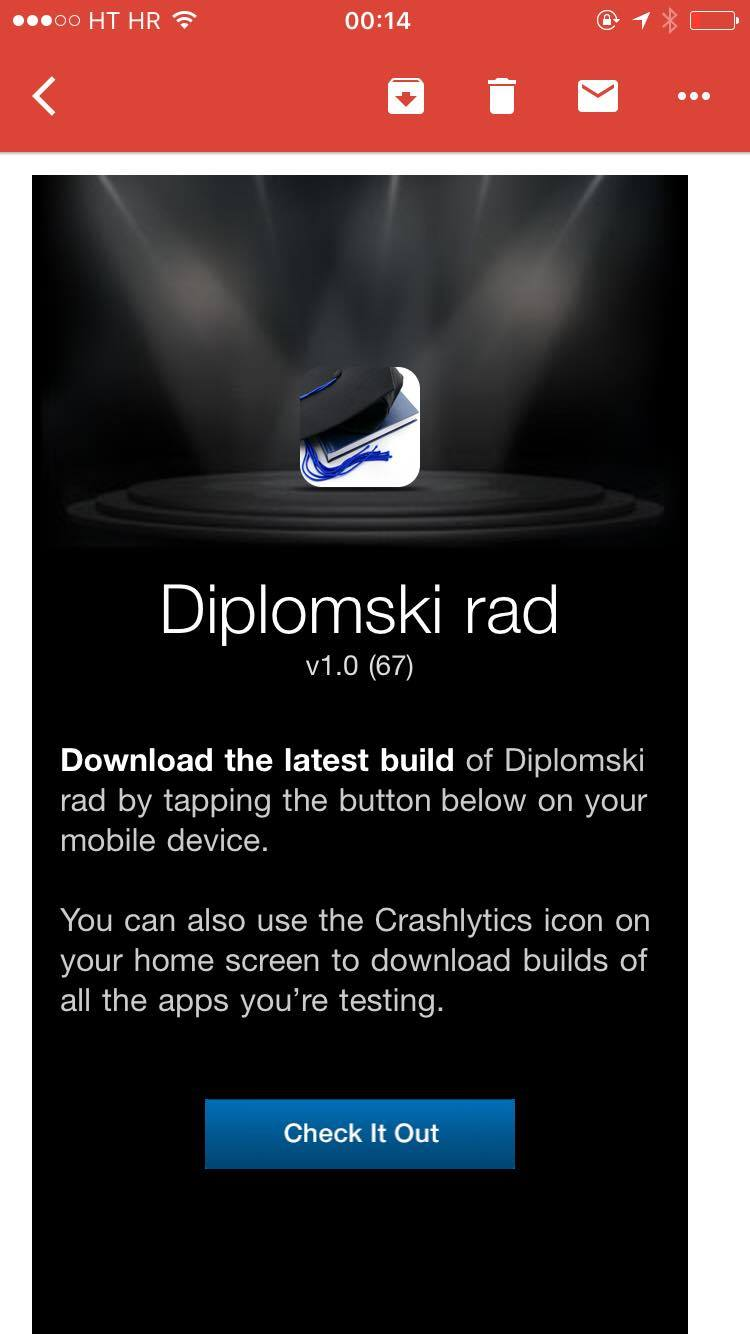
\includegraphics[scale=0.3]{CrashlyticsEmail}
\caption{Crashlytics e-mail poruka izdana nakon objave nove verzije aplikacije}
\label{fig:CrashlyticsEmail}
\end{figure}

\begin{lstlisting}[caption=Fastlane staza za isporuku korištenjem Crashlytics platforme, label=listing:crashlytics_deploy]
lane :develop do
    increment_build_number

    match(app_identifier: "com.rep.Diplomski-rad.development", type: "development")
    gym(scheme: "Diplomski_rad", export_method: "development")

    crashlytics(
        api_token: {api_kljuc},
        build_secret: {tajni_kljuc},
        groups: 'Rep'
    )

end
\end{lstlisting}

Dodatno, kako prilikom pokretanja naredbe ne bi morao unositi crashlytics API i tajni ključ, iste je moguće specificirati kao argumente crashlytics naredbe.

Nakon isporuke je aplikaciju moguće preuzeti direktno s Crashlytics platforme. Kako bi korisnik mogao preuzeti aplikaciju, potrebno ga je prvo dodati kao testera pojedine aplikacije. Na Crashlytics profilu aplikacije odabrati \verb|Add testers| opciju te unijeti email adresu željene osobe. Na uređaju otvoriti dobivenu e-mail poruku te odabrati opciju \verb|Let Me In|. Slika \ref{fig:CrashlyticsEmail} prikazuje dobivenu e-mail poruku.

Crashlytics instalaciju aplikacija objavljenih na Crashlytics platformi obavlja pomoću aplikacije \textit{Beta}. Ako ista nije instalirana poveznica pokreće proces instalacije i konfiguracije pomočne aplikacije. Slika \ref{fig:Beta} prikazuje ekran za preuzimanje aplikacije. Odabirom opcije \verb|Install| se pokreće instalacija nanovije verzije aplikacije. Moguće je također preuzeti neku od starijih verzija aplikacije.

\begin{figure}[h!]
\centering
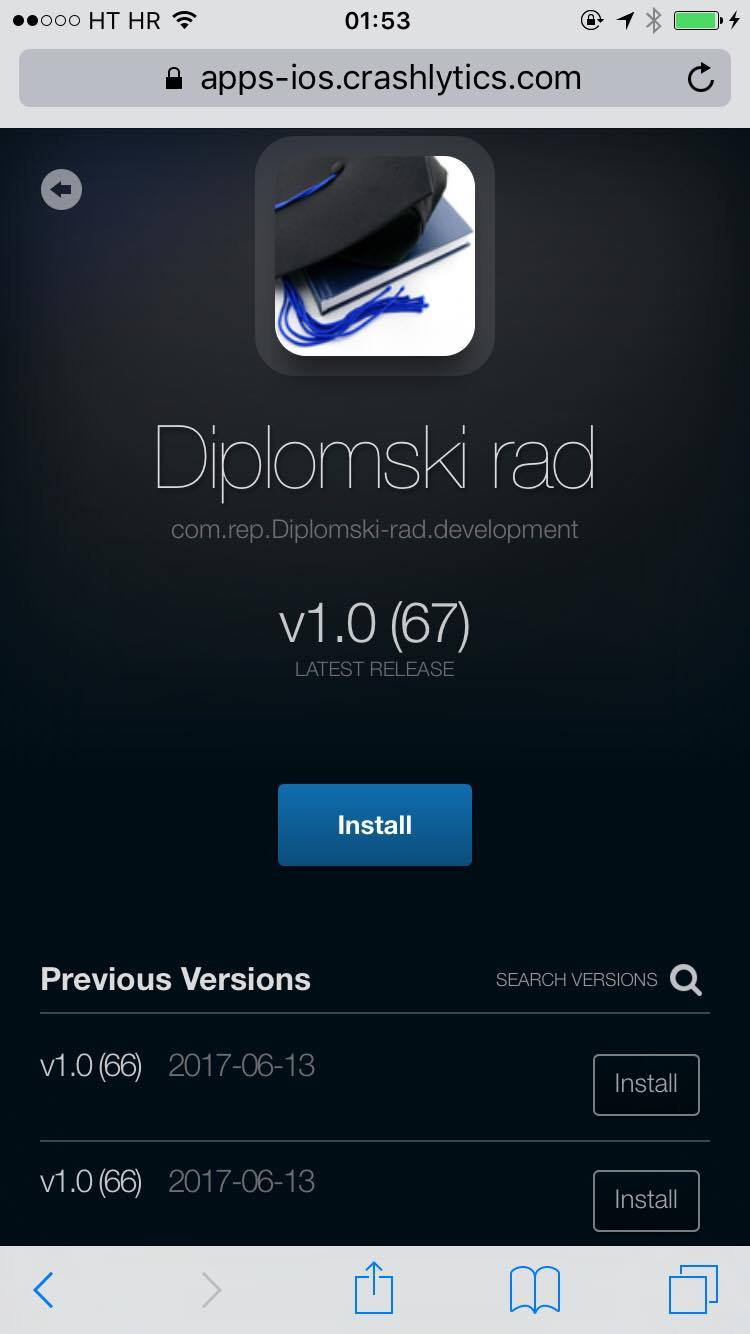
\includegraphics[scale=0.3]{Beta}
\caption{Preuzimanje aplikacije s Crashlytics platforme korištenjem aplikacije Beta}
\label{fig:Beta}
\end{figure}

Ako je aplikacija isporučena korištenjem ad hoc isporuke, uređaj korisnika mora biti registriran kao testni uređaj te dodan ad hoc profilu. Kako ne bi morali svakoj verziji aplikacije dodavati testere, grupa testera se može dodati kao argument Crashlytics naredbi \verb|groups: {ime_grupe}|.


\subsection{App Store}

Objava javnih iOS aplikacija se ostvaruje korištenjem App Store platforme. App Store je službena platforma za distribuciju programske potpore za macOS, iOS, tvOS i watchOS operacijske sustave. Uz dostupnost aplikacije svim korisnicima navedenih operacijskih sustava, platforma pruža i brojne druge funkcionalnosti kao što su automatsko instaliranje novih verzija aplikacija i praćenje ponašanja korisnika.

Objava programske potpore na App Store platformu se obavlja korištenjem iTunes Connect web stranice. iTunes Connect omogućava kreiranje, modificiranje i praćenje objavljene programske potpore. Prije objave je potrebno kreirati profil aplikacije korištenjem iTunes Connect alata.

Kreiranje profila se obavlja na \path|https://itunesconnect.apple.com/| stranici. Nakon prijave je potrebno odabrati opciju \verb|My Apps| te kreirati novi profil. Slika \ref{fig:iTunesConnectAppCreation} prikazuje formu za kreiranje profila aplikacije.

\begin{figure}[b!]
\centering
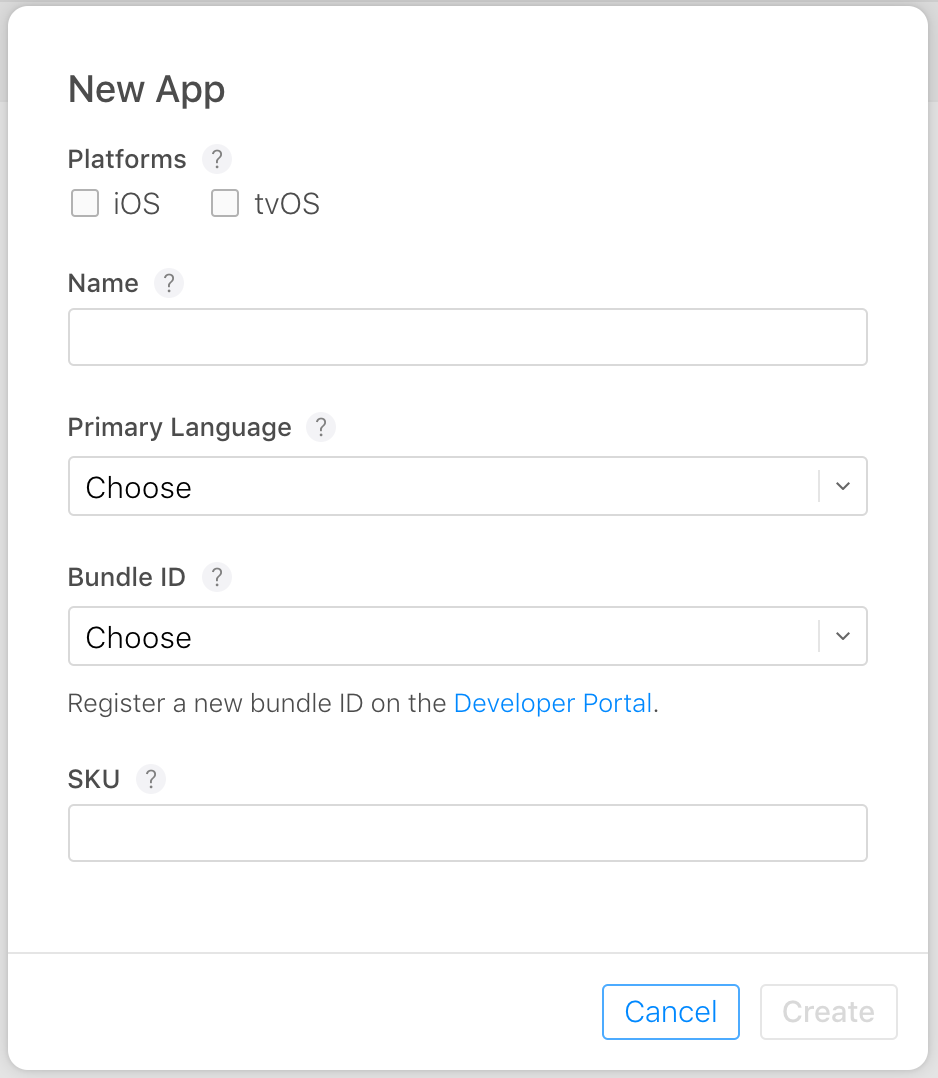
\includegraphics[scale=0.4]{iTunesConnectAppCreation}
\caption{Forma za kreiranje profila aplikacije na iTunes Connect web stranici}
\label{fig:iTunesConnectAppCreation}
\end{figure}

Nakon kreiranja profila aplikacije je potrebno ispuniti dodatne podatke o aplikaciji kao što su opis i kategorija aplikacije. Slično kao i kod Crashlytics platforme, sada je moguće jednostavno dostaviti arhivu i manifest aplikacije.

Iako isporuka aplikacija korištenjem App Store platforme donosi brojne prednosti, ona donosi i brojne nedostatke. Ovaj tip isporuke je poprilično složen te traje puno duže u usporedbi s ostalim tipovima isporuke. Apple vrlo strogo regulira aplikacije koje se nalaze na App Store platformi.

Proces provjere aplikacije zna trajati i do nekoliko tjedana te često rezultira odbijanjem aplikacije. Aplikacija može biti odbijena jer je previše slična već postojećoj aplikacije, jer se ne slaže s nekom od Appleovih politika, zbog loše implementacije i brojnih drugih razloga. Nakon otklanjanja razloga odbijanja je potrebno ponovno proći cijeli proces.

Za objavu nove verzije aplikacije je potrebno proći nešto blažu provjeru. Ona može trajati od nekoliko sati do nekoliko dana te najčešće završava odobrenjem promjena. Odbijanje promjena je vrlo rijetko te služi prvenstveno za prevenciju očitog narušavanja Appleovih politika.

Ovaj proces isporuke je složen i dugotrajan. Iako se u zadnjih nekoliko godina proces značajno poboljšao, veliki broj članova industrije je još uvijek vrlo nezadovoljan. Međutim, Apple zabranjuje isporuku aplikacija za javnu uporabu korištenjem bilo koje druge metode. Ako navedeni proces usporedimo s procesom isporuke web aplikacija, onda su njegovi nedostaci jasno vidljivi. Nova verzija web aplikacije se isporučuje jednostavno promjenom verzije koja se nalazi na poslužitelju. Prvi sljedeći korisnik koji pristupi služitelju automatski koristi sljedeću verziju. Ne samo da je proces isporuke iOS aplikacija daleko teži i sporiji, već korisnik mora samostalno preuzeti novu verziju aplikacije.

Apple nastoji što jednostavnije i neprimjetnije osvježiti verzije aplikacije. Aplikacije se automatski osvježuju kad je uređaj spojen na WiFi mrežu te je dovoljno napunjen. Međutim, određeni broj korisnika isključuje ovu funkcionalnost ili ručno odobrava svaku novu verziju aplikacije. Zbog navedenog uvijek postoji određeni postotak korisnika koji vrlo dugo koriste starije verzije aplikacije. Navedeno iziskuje dugoročnu podršku starijih verzija aplikacije što značajno otežava razvoj.

Zbog navedenih razloga prominenti pojedinci u iOS zajednici predviđaju skoru zamjenu App Store platforme nekim boljim načinom isporuke. Međutim, Apple nije objavio nikakvu naznaku ovog te smo za sad ograničeni sustavom koji imamo.

\paragraph{Automatizacija objave}

Isporuku programske potpore za App Store platformu implementiram pomoću fastlane dodatak \verb|deliver|\citep{fastlane:deliver}. Dodatak korištenjem javnog APIa iTunes Connect platforme automatizira dostavu arhive i manifesta. Alat se direktno nadovezuje na alat gym, samostalno detektira potrebne artefakte te omogućava jednostavnu konfiguraciju procesa.

Inicijalizacija deliver dodataka je prikazana u skripti \ref{listing:deliverInit}. Naredba projekt povezuje s iTunes Connect platformom kako bi ubuduće dodatak mogao samostalno obaviti objavu. Za autorizaciju pristupa je potrebno je korisničko ime i lozinku Apple Developer računa. Inicijalizaciju dovršiti unosom iTunes identifikatora profila aplikacije. Identifikator je moguće dohvatiti korištenjem iTunes Connect platforme. Nakon prijave na web stranicu \path{https://itunesconnect.apple.com} odabrati opciju \verb|My Apps| te odabrati željenu aplikaciju. Slika \ref{fig:iTunesConnectAppId} prikazuje lokaciju identifikatora aplikacije na profilu aplikacije.

\begin{lstlisting}[caption=Inicijalizacija deliver dodatka, label=listing:deliverInit]
fastlane deliver init
\end{lstlisting}

\begin{figure}
\centering
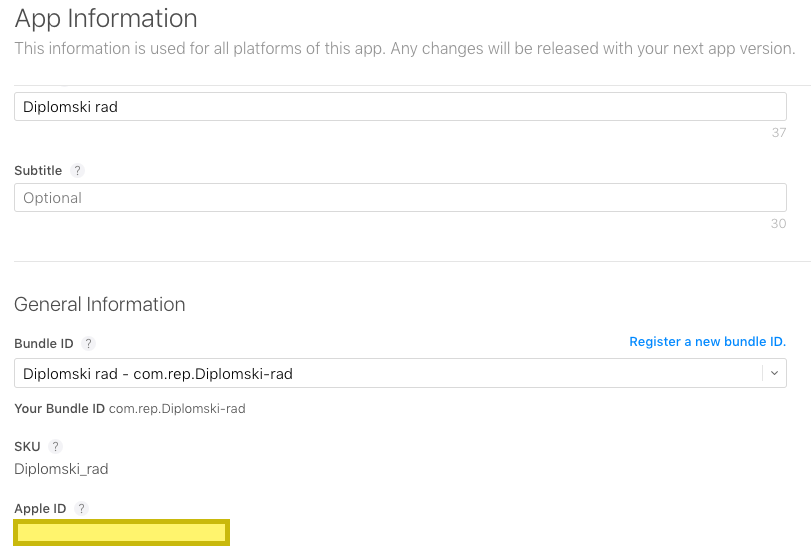
\includegraphics[scale=0.4]{iTunesConnectAppId}
\caption{iTunes Connect profil aplikacije s označenim identifikatorm aplikacije}
\label{fig:iTunesConnectAppId}
\end{figure}

Naredba kreira nekoliko datoteka u \verb|fastlane| direktoriju. Tekstualna datoteka \verb|Deliverfile| pohranjuje podatke vezane uz objavu aplikacije na App Store platformi kao što su korisničko ime Apple Developer računa te identifikator aplikacije. Direktorij \verb|metadata| sadrži nekoliko dokumenata koji omogućavaju jednostavan unos podataka koji će se koristiti prilikom isporuke aplikacije na App Store platformu. Na primjer, pomoću dokumenta \verb|description.txt| je moguće specificirati opis aplikacije. Dodatno, moguće je kreirati zaseban opis za svaki jezik koji Apple podržava.

Sada je isporuku moguće obaviti jednostavno pozivom \verb|deliver| alata. Naravno, kreirana arhiva mora biti potpisana certifikatima i profilima za distribuciju na App Store platformi. Zbog navedenog kreiram novu shemu pomoću koje specificiram korištenje ispravnih certifikata i profila.

Staza u nastavku implementira objavu aplikacije na App Store platformu.

\begin{lstlisting}[caption=Isporuka na App Store platformu korištenjem dodatka deliver]
lane :release do
match(type: "appstore")
gym(scheme: "Production", export_method: "app-store")
deliver
end
\end{lstlisting}

Staza prvo dohvaća potrebne certifikate i profile, izgrađuje arhivu aplikacije te na kraju arhivu objavljuje koristeći deliver dodatak.

Nakon isporuke aplikacije je moguće pokrenuti proces objave. Prije objave, aplikacija mora proći Appleov pregled koji može trajati i do nekoliko tjedana. Zbog navedenog je preporučeno prije pokretanja procesa detaljno provjeriti ispravnost aplikacije te pročitati službene smjernice. Ako aplikacija prođe provjeru, onda ju je moguće objaviti korištenjem iTunes Connect web stranice.




Objavu \textit{ad hoc} i unutarnje verzije arhiva ostvarujem korištenjem Crashlytics platforme. Platforma omogućava jednostavnu objavu arhiva, kontrolu pristupa i osvježenje verzija. Jednostavno je na platformu dodati nove korisnike i istima dopustiti preuzimanje aplikacije. Dodatno, korisnici korištenjem aplikacije \verb|Beta| mogu jednostavno vidjeti, preuzeti i osvježiti sve aplikacije kojima je dobio pristup.

Crashlytics platforma pruža javan API koji je moguće iskoristiti za kreiranje profila i dodavanje nove verzije aplikacije. Dodatno, moguće je korisnicima dati pristup profilu aplikacije te iste obavijestiti o novoj verziji. Za ostvarenje navedenih funkcionalnosti koristim alat \verb|crashlytics| familije \verb|fastlane|.

Aplikaciju za javne korisnike objavljujem na App Store platformi. Prije objave aplikacije je potrebno kreirati njen profil. Profil se kreira korištenjem iTunes Connect aplikacije. Nakon kreiranja profila je moguće dodati prvu verziju aplikacije. Budući da prva verzija aplikacije prolazi strogu provjeru, nije preporučeno njeno automatizirano dodavanje. Prva se verzija najčešće ručno provjerava, arhivira u objavljuje.

Automatizacije objave se ostvaruje korištenjem javnog APIja iTunes Connect platforme. Za jednostavniju implementaciju koristim \verb|deliver| alat \verb|fastlane| familije. Alat specificiranu arhivu objavljuje na iTunes Connect platformi. Nova verzija također prolazi provjeru Apple time. U slučaju odobrenja nove verzije istu je potrebno objaviti u produkciji. Navedeno je moguće ostvariti korištenjem iTunes Connect platforme ili APIja.



\chapter{Kontinuirana isporuka} \label{header:KontinuiranaIsporuka}

Kontinuirana isporuka \eng{continuous deployment} je praksa u programskom inženjerstvu koja nastoji smanjiti vrijeme između razvoja i objave funkcionalnosti u produkciju. Kontinuirana dostava automatizira proces isporuke, međutim, ne isporučuje programsku potporu automatski. Svaku isporuku nove verziju programske potpore je potrebno ručno pokrenuti. S druge strane, kontinuirana isporuka automatski isporučuju svaku novu verziju. Razlika između kontinuirane dostave i kontinuirane isporuke je prikazana na slici \ref{fig:CDDifferences}\citep{cd:whats_the_diff}.

\begin{figure}
\centering
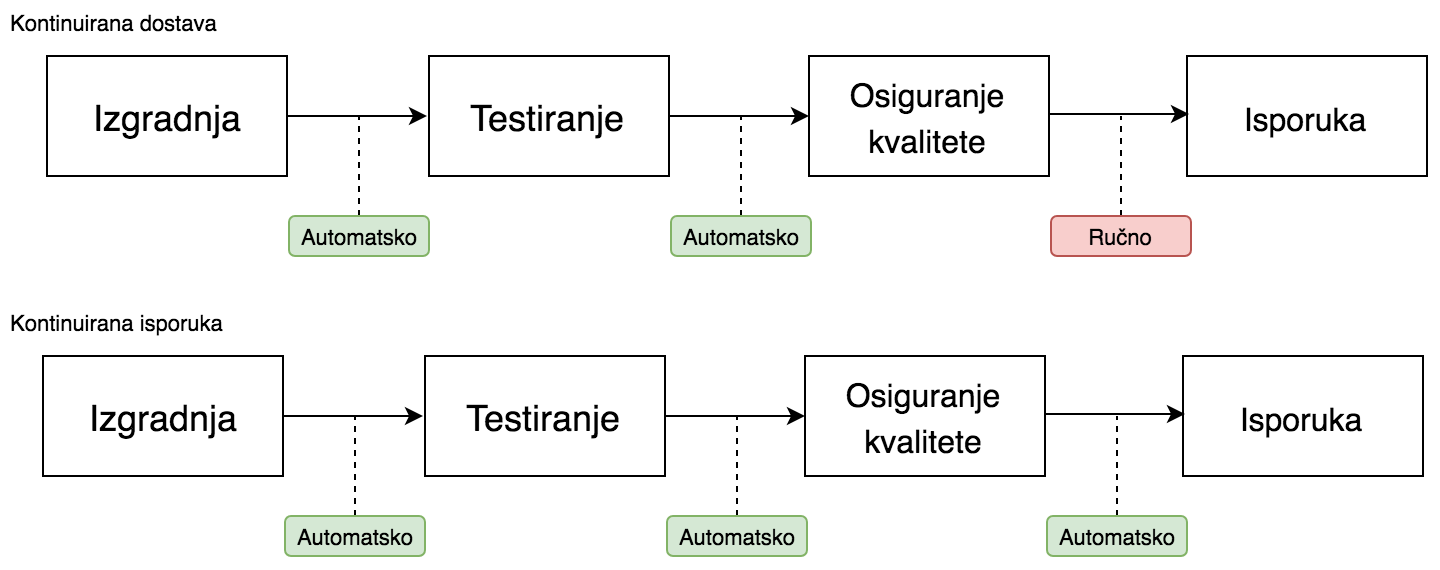
\includegraphics[scale=0.55]{CDDifferences}
\caption{Usporedba kontinuirane dostave i kontinuirane isporuke}
\label{fig:CDDifferences}
\end{figure}

Kontinuirana isporuka automatskom isporukom promjena u produkciju nastoji smanjiti vrijeme između razvoja funkcionalnosti i njene objave u produkciju te samim time ukupno vrijeme trajanja razvoja. Kontinuirana isporuka ova obavlja na dva načina. Prvo, automatizacijom isporuke i automatskom isporukom promjena, kontinuirana isporuka značajno smanjuje vrijeme koje tim mora uložiti za obavljanje isporuke. Druga stavka je direktna posljedica prve. Zbog smanjenja opterećenja koje isporuka nanosi na tim, obavljanje isporuke postaje puno lakše. Lakše obavljanje isporuke dovodi do češćeg obavljanja isporuke. Irska kompanije \textit{Intercom} u svom blogu bilježi stabilan porast broja dnevnih isporuka promjenu od produkcija. Od ispod 20 isporuka u 2012. godini, do preko 80 isporuka u 2015. godini. Slika \ref{fig:IntercomShipsPerDay} prikazuje broj dnevnih isporuka promjena u produkciju kompanije \textit{Intercom}\citep{intercom:cd}.

\begin{figure}
\centering
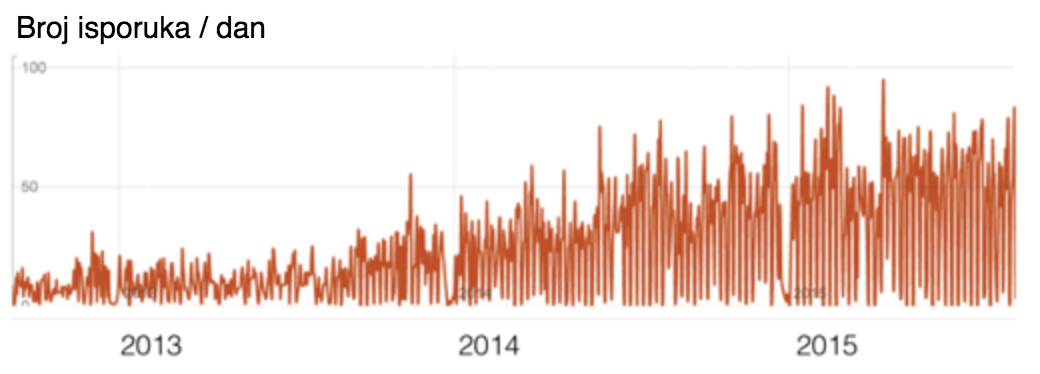
\includegraphics[scale=0.7]{IntercomShipsPerDay}
\caption{Broj dnevnih isporuka promjena u produkciju kompanije \textit{Intercom}}
\label{fig:IntercomShipsPerDay}
\end{figure}

Iako kontinuirana isporuka nastoji promjene automatski isporučiti u produkciju, navedeno ne znači da se svaka promjena koda automatski isporučuju direktno korisniku. Prvo, svaka promjena prolazi cijeli proces automatskog testiranja i provjere kvalitete. Dodatno, promjene u praksi često prolaze brojna ručna testiranja prije objave u produkciju. Ručna testiranja možemo generalno podijeliti na testiranja razvojnog tima, testiranja tima za osiguranje kvalitete i testiranja vanjskih korisnika koja po broju korisnika dijelimo na \textit{alpha} i |textit{beta} testove.

Dok se \textit{alpha} testiranja provode na vrlo malom broju korisnika, \textit{beta} testiranja mogu sadržavati i do 10% korisnika. Testiranja razvojnog tima provodi tim koji razvija aplikaciju. Ovi testovi nastoje potvrditi ispravnost razvijene funkcionalnosti ali ne ulaze dulje u ispravnost cijele programske podrške. Testiranja tima za osiguranje kvalitete nastoje osigurati ispravnost cijele programske podrške. Način, raspored i provođenje testiranja je strogo definiran te po opsegu daleko nadmašuje testiranje razvojnog tima. S druge strane, testiranja na vanjskim korisnicima ne provode zaposlenici već potencijalni budući korisnici. Korisnici ne testiraju programsku podršku već ju normalno koriste. Međutim, velik broj korisnika omogućava pronalazak i najmanje greške u programskoj podršci. Dodatno, ovaj tip testiranja se može iskoristiti i za praćenje ponašanja korisnika na temelju čega se mogu uvoditi poboljšanja produkta.

Umjesto da se programska podrška isporuči direktno korisnicima, ona prolazi niz ručnih testiranja. Primjer procesa isporuke produkta različitim skupinama korisnika je prikazana na slici \ref{fig:DeploymentStages}.

\begin{figure}[h]
\centering
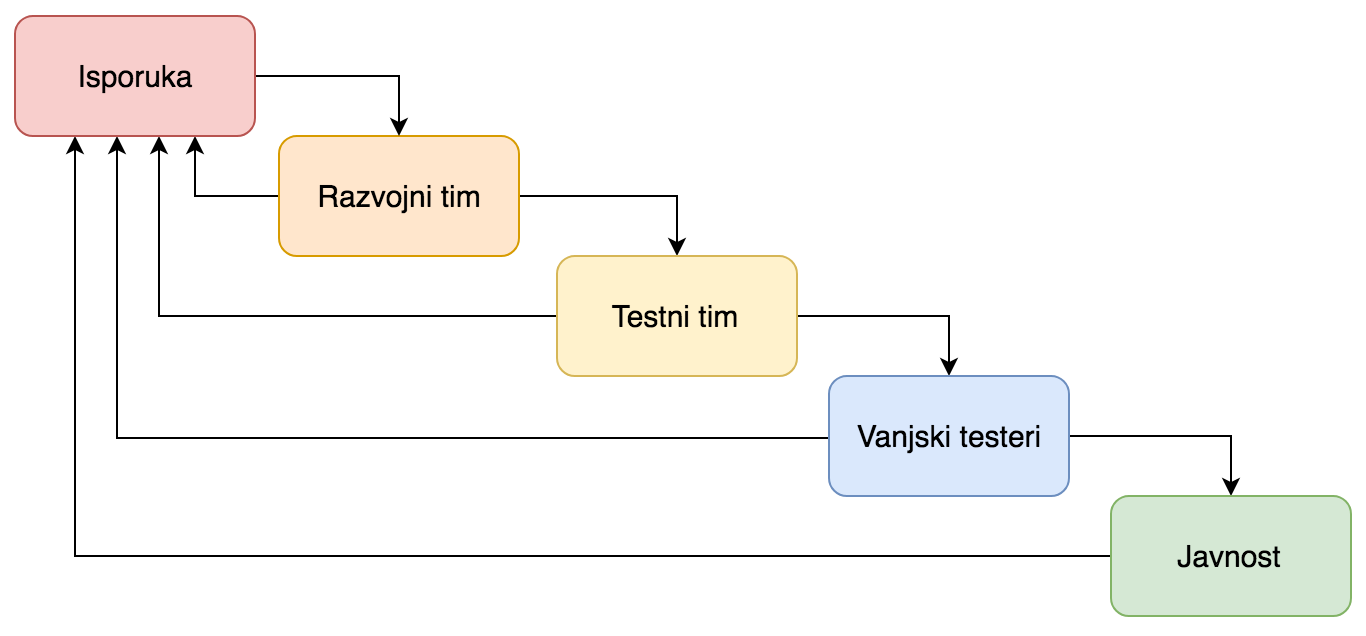
\includegraphics[scale=0.6]{DeploymentStages}
\caption{Postupna isporuka programske potpore skupovima korisnika}
\label{fig:DeploymentStages}
\end{figure}

Termin kontinuirana isporuka je prvi puta iskoristio poznati autor Kent Beck u razgovoru o agilnom razvoju. Kent Beck je neisporučenu funkcionalnost usporedio s inventarom koji nije prikazan korisniku. Termin je prvi puta definiran u članku \textit{The Deployment Production Line} autora Jez Humblea, Chris Reada i Dan Northa. Praksa je postala posebno prihvaćena zajednici. Danas praksu razvija i unaprjeđuje uglavnom zajednica web programera koji ju, zbog jednostavnosti isporuke programske podrške za web poslužitelje, mogu jednostavno implementirati.

Isporuka programske podrške za web poslužitelje ima značajnu prednost u usporedbi s ostalom programskom potporom. Najvažnije, web aplikacije nije potrebno instalirati na uređaj. Korisnik promjene vidi čim su one dodane na poslužitelju. Dodatno, razvojni tim može direktno upravljati koju će verziju programske potpore korisnik vidjeti. U usporedbi, isporuka iOS aplikacija prvo mora proći provjeru Apple tima te je korisnik mora preuzeti na uređaj. Zbog navedenog se kontinuirana isporuka programske potpore za iOS operacijski sustav značajno razlikuje od tradicionalne kontinuirane isporuke.


\section{Kontinuirana isporuka za iOS operacijski sustav}

Kontinuirana isporuka za iOS operacijski sustav se značajno razlikuje od tradicionalne prakse kontinuirane isporuke. Glavni razlog ove razlike je App Store platforma. Dok se nova verzija web aplikacije može isporučiti u nekoliko minuta, nova verzija iOS aplikacije mora proći službenu provjeru Apple tima te ju potom korisnik mora preuzeti. Dodatno, App Store je zatvorena platforma s ograničenim skupom funkcionalnosti. Iako Apple konstantno dodaje nove funkcionalnosti, platforma je u velikom zaostatku u usporedbi s web razvojem. Navedena ograničenost App Store platforme je glavni razlog zbog kojeg veliki broj poznatih članova iOS zajednice prognozira njenu postupnu eliminaciju. Iako App Store platforma ima navedena ograničenja, još uvijek je moguće automatizirati veliki dio procesa.

Isporuka programske potpore za ograničene skupove korisnika je puno jednostavnija. Budući da za ovaj tip isporuke nije potrebno koristiti App Store platformu, moguće je ostvariti puno veći set funkcionalnosti. U sklopu ovog rada koristim Crashlytics platformu koja pruža brojne funkcionalnosti kao što su automatsko osvježenje i postupna isporuka aplikacije korisnicima.

Vratimo se sada na projekt za koji implementiram kontinuiranu isporuku. U sklopu razvoja isporučujem četiri različite verzije aplikacije pod nazivima: razvoja \eng{develop}, testna \eng{test}, pripremna \eng{release candidate} i produkcijska \eng{production} aplikacija.

Razvojna aplikacije prikazuje trenutno stanje aplikacije. Koriste je članovi tima kako bi mogli isprobati novo razvije funkcionalnosti te kako bi mogli pratiti napredak projekta. Svaka završena izmjena treba biti u što kraćem roku vidljiva na ovoj verziji aplikacije.

Testnu aplikaciju koristi tim za osiguranje kvalitete kako bi osigurao ispravnost novo razvijenih funkcionalnosti. Kako bi osigurao ispravnost tim provjerava sve izmjene ostvare od zadnje verzije aplikacije. Zbog navedenog je poželjno da je broj izmjena između verzija mali ali dobro dokumentiran. Verzija ovog tipa aplikacije se osvježava otprilike jednom tjedno.

Pripremna aplikacije služi za pripremu aplikacije za izdavanje u produkciju. Sve izmjene obavljene od zadnje verzije se još jednom provjeravaju kako bi izbjegli pojavu grešaka u produkcijskoj aplikaciji. Osim tima za osiguranje kvalitete, pristup ovom tipu aplikacije često imaju i vanjski korisnici. Nova verzija ovog tipa aplikacije se kreira kada je potrebno isporučiti aplikaciju u produkciju.

Produkcijska aplikacija je aplikacija trenutno dostupna korisniku. Verzija se osvježava jednom do dva put u tri mjeseca.

Iz navedenog je jasno da trenutan proces ne slijedi principe kontinuirane isporuke. Između dvije produkcijske verzije može proći i tri mjeseca. Ovaj spor proces izdavanja promjena u produkciju rezultira većim brojem ljudskih pogrešaka i lošijim iskustvom korisnika. Zbog navedenog automatizacijom procesa ne samo da pokušavam smanjiti vrijeme koje tim ulaže u isporuku, već i smanjiti period između dvije isporuke.


\section{Pokretanje isporuke}

Iako je cilj kontinuirane integracije svaku promjenu što brže isporučiti, nema smisla za svaku promjenu linije koda graditi novu verziju aplikacije. Ne samo da to ne bi bilo resursno isplativo, već većina verzija ne bi prošla nit proces automatskog testiranja i provjere kvalitete. Pametnije je verziju prilikom spremanja promjena u repozitoriju izvornog koda.

Dodatno, u praksi se često jedna funkcionalnost razdvaja na više manjih promjena. Svaka od ovih promjena sama prolazi automatska testiranja i osiguranje kvalitete, međutim često dovodi aplikaciju u neupotrebljivo stanje. Zbog navedenog nema smisla osvježavati verziju kada se ona nalazi u navedenom među stanju. Dodatno, razvojni tim može istovremeno raditi na nekoliko različitih funkcionalnosti.

Za rješavanje navedenog problema se u praksi najčešće koristi proces verzioniranja poz nazivom grananje funkcionalnosti \eng{feature branch} opisana u odlomku \ref{header:Implementacija_verzioniranja}. Umjesto pokretanja procesa isporuke aplikacije prilikom svake promjene repozitorija izvornog koda, proces isporuke se pokreče samo prilikom izmjene glavne grane. Ovaj pristup smanjuje opterećenje sustava te rezultira isporukom upotrebljivog produkta. Dodatno, prilikom spajanja razvojne grane je moguće obaviti dodatne kontrole ispravnosti kao što su timski pregled koda. Slika \ref{fig:FeatureBranchCD} prikazuje proces automatskog pokretanja isporuke nakon spajanja razvojne grane.

\begin{figure}
\centering
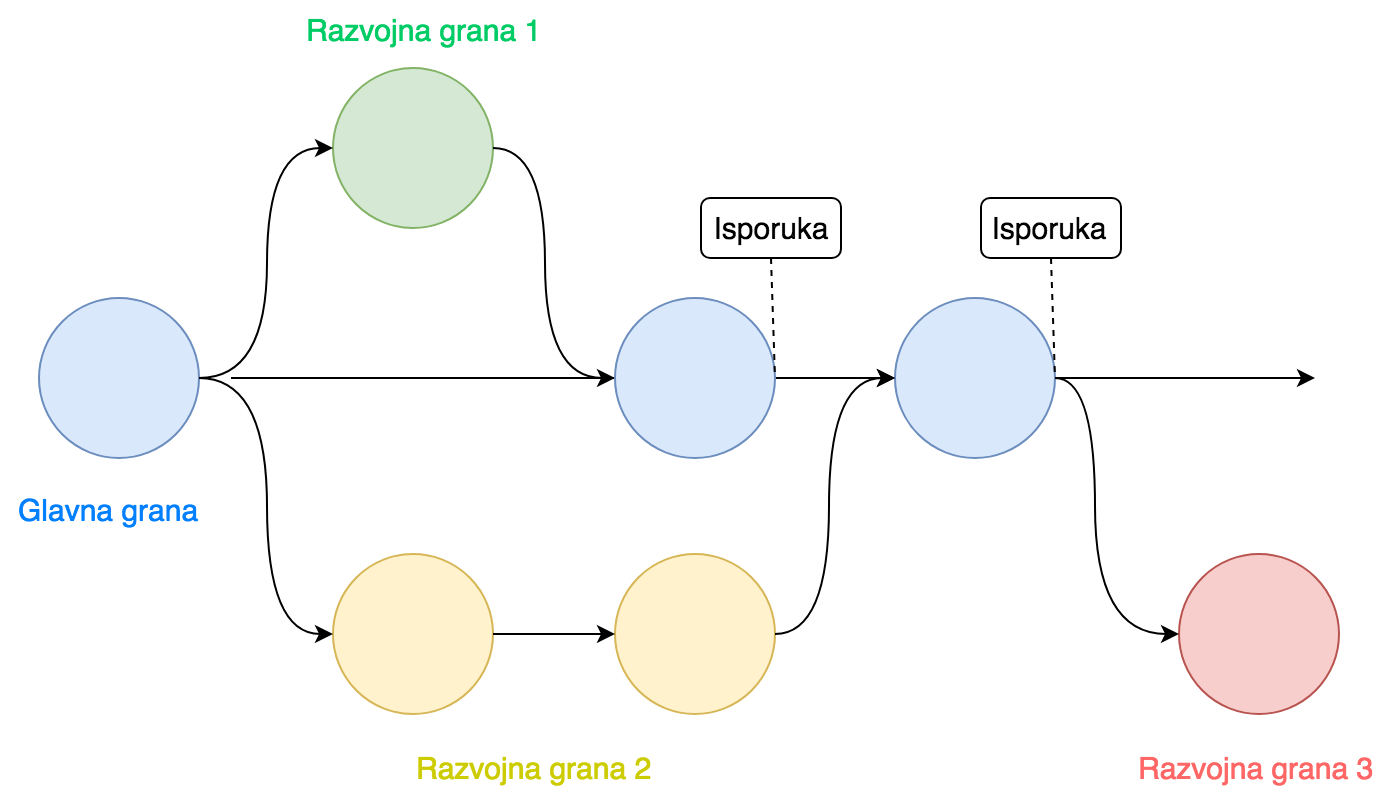
\includegraphics[scale=0.5]{FeatureBranchCD}
\caption{Automatska isporuka nakon promjene glavne grane}
\label{fig:FeatureBranchCD}
\end{figure}

Ovaj pristup je vrlo jednostavan te omogućava automatiziranje isporuke promjena na produkciju. Ako projekta ne zahtijeva testnu i pripremnu verziju aplikacije, isporuku u produkciju je moguće ostvariti korištenjem oznaka \eng{tag}. Oznake dodaju dodatno značenje stanju u sustavu za kontrolu verzija. Umjesto isporuke na temelju novog stanja, isporuku u produkciju je moguće pokrenuti nakon kreiranja oznake.

Međutim, ovaj tip automatske isporuke je vrlo limitiran. Glavna mana je limitiranost u broju tipova aplikacija. Za otklananje navedenog problema možemo koristiti \textit{gitflow} proces verzioniranja. Umjesto postojanja jedne glavne grane, \textit{gitflow} proces koristi nekoliko grana s posebnim značenjem.

Glavna grana \eng{master branch} predstavlja trenutno stanje programske potpore u produkciji. Svaka verzija ove grane je obilježena oznakom koja sadrži ljudski čitljivu verziju aplikacije i popis promjena obavljenih od prošle verzije. Razvojna grana \eng{develop branch} predstavlja trenutno stanje aplikacije u razvoju. Objava promjena u produkciju se obavlja pomoću pomoćne grane koja se kreira iz razvojne grane. Nakon provjere ispravnosti promjena iste se dodaju glavnoj grani i time objavljuju u produkciju. Pregled cijelog procesa je dostupan u odlomku \ref{header:Implementacija_verzioniranja}.

Za potrebe našeg projekta koristim modificiranu verziju \textit{gitflow} procesa. Uz glavnu i razvojnu granu koristim još dvije posebne grane. Testna grana služi za isporuku testne aplikacije timu za osiguranje kvalitete. U testnu se granu promjene dodaju iz razvojne grane. Nakon pronalaska pogreške iste se otklanjaju direktno na ovoj grani. Nakon potvrde ispravnosti funkcionalnosti započinje testiranje novonastalih funkcionalnosti.

Pripremna grana služi za pripremu isporuke aplikacije u produkciju. Grana se kreira iz željenog ispravnog stanja testne grane. Nakon završne provjere ispravnosti promjene se dodaju na glavnu granu čime se objavljuju u produkciju. Slika \ref{fig:GitFlowCD} prikazuje proces automatizirane isporuke korištenjem \textit{gitflow} procesa.

\begin{figure}
\centering
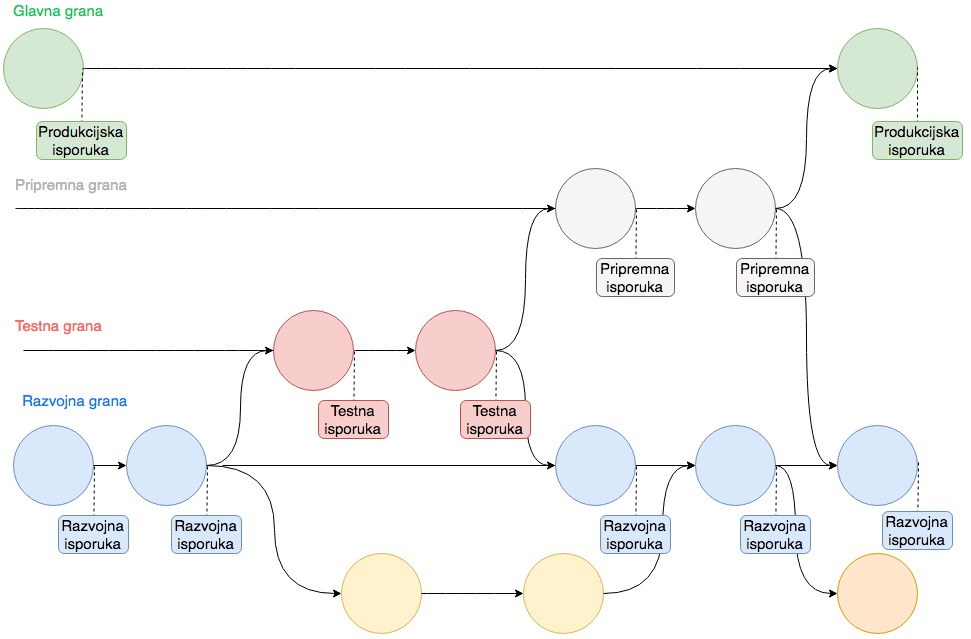
\includegraphics[scale=0.5]{GitFlowCD}
\caption{Automatska isporuka primjenom \textit{gitflow} procesa}
\label{fig:GitFlowCD}
\end{figure}

\begin{figure}
\centering
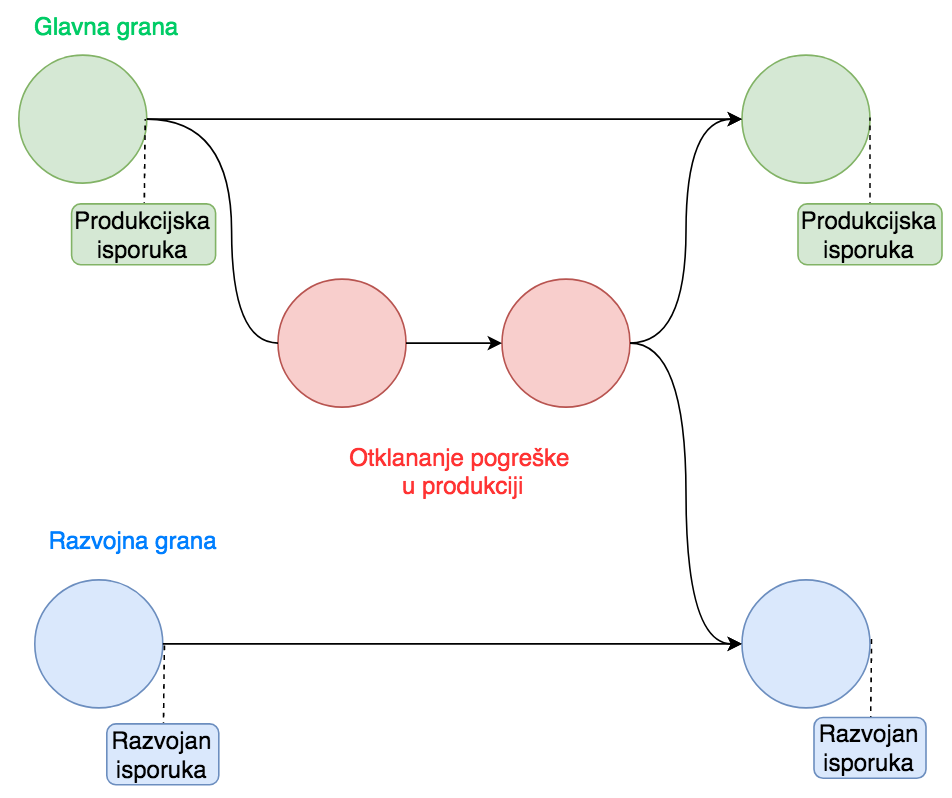
\includegraphics[scale=0.5]{HotfixGitflow}
\caption{Automatska isporuka otklananja pogreške u produkciji}
\label{fig:HotfixGitflow}
\end{figure}

U praksi se često javljaju novi, neočekivani zahtjevi. Jedan od primjera ovog tipa zahtjeva je otkrivanje pogreške u produkcijskoj verziji koju je odmah potrebno ukloniti. Budući da razvojna grana sadrži promjene koje još nisu objavljene na produkciji, grešku nije moguće otkloniti sljedeći standardnu praksu. Međutim, moguće je granu za otklanjanje pogreške kreirati direktno iz glavne grane. Nakon otklanjanja pogreške i testiranja, promjena se spaja s glavnom granom čime se ista objavljuje u produkciju i s radnom granom. Primjer otklanjanja greške u produkciji se nalazi na slici \ref{fig:HotfixGitflow}. Važno je prilikom pojave zahtjeva ovog tipa iskoristiti postojeće procese isporuke.


\section{Implementacija kontinuirane isporuke}

Za ostvarenje kontinuirane isporuke je potrebno pokrenuti odgovarajući proces kontinuirane dostave ako se proces kontinuirane integracije uspješno izvrši. Budući da su kontinuirana integracija i kontinuirana dostava već implementirani, potrebno je samo detektirati uspješnost izvršenja kontinuirane integracije i pokrenuti odgovarajući proces kontinuirane dostave.

Provjeru ispravnog izvršenja kontinuirane integracije obavljam korištenjem varijabli okruženja koje Xcode Server generira u procesu integracije.

Ispravnost izgradnje provjeravam korištenjem varijabli \verb|XCS_ERROR_COUNT|, \\ \verb|XCS_WARNING_COUNT| i \verb|XCS_WARNING_CHANGE|. \verb|XCS_ERROR_COUNT| i \\ \verb|XCS_WARNING_COUNT| varijable definiraju broj pogrešaka i upozorenja generiranih u procesu integracije. Za ispravnost izgradnje broj grešaka mora biti 0. Poželjno je da i broj upozorenja bude 0, ali zbog vanjskih biblioteka to često nije moguće ostvariti. Zbog navedenog se umjesto broja upozorenja često koristim \verb|XCS_WARNING_CHANGE| varijablu koja definira promjenu u broju upozorenja. U sklopu ovog projekta definiram da je izgradnja uspješna ako se broj upozorenja nije povećao.

Ispravnost testiranja provjeravam korištenjem \verb|XCS_TEST_FAILURE_COUNT| varijable. Testiranje smatram uspješnim isključivo ako je broj neuspješnih testova 0.

Ispravnost provjere ispravnosti ovisi o definiranim provjerama ispravnosti. Swiftlint nepoštivanje pravila dojavljuje koristeći standardne pogreške i upozorenja. Trenutno nije moguće razaznati je li pogreška ili upozorenje generirano izgradnjom ili Swiftlint provjerom. Zbog navedenog se držim pravila definiranog u sklopu ispravnosti izgradnje. Pokrivenost koda trenutno nije dostupna putem varijable okruženja. Međutim, moguće ju je dohvatiti korištenjem javnog Xcode Server APIja pozivom \verb|GET HTTPS| metode:

\begin{verbatim}
/integration/{id}/coverage{?include_methods}
\end{verbatim}

Naredba vraća podatke o pokrivenosti koda u JSON formatu koje je moguće iskoristiti za provjeru dovoljne pokrivenosti koda testovima.

Provjeru ispravnost cijele integracije implementiram koristeći sljedeću naredbu:

\begin{verbatim}
if XCS_ERROR_COUNT == 0 &&
    XCS_WARNING_CHANGE <= 0 &&
    XCS_TEST_FAILURE_COUNT == 0
        {isporuka}
fi
\end{verbatim}

Tip isporuke koji se koristi je moguće definirati direktno u botu koji koristimo, na temelju imena bota ili imena izvorne grane. Definiranje tipa isporuke u samom botu je najjednostavnije, ali uzrokuje razlikom u implementaciji botova. U radu koristim ime bota pohranjeno u varijabli okruženja \verb|XCS_BOT_NAME|. Na temelju imena odlučujem koji proces isporuke pokrenuti.

\begin{verbatim}
if XCS_BOT_NAME == '*Test'
    fastlane test
elif XCS_BOT_NAME == '*ReleaseCandidate'
    fastlane release_candidate
elif XCS_BOT_NAME == '*Production'
    fastlane production
else
    fastlane develop
fi
\end{verbatim}


\chapter{Zaključak}
Zaključak.

\bibliography{literatura}
\bibliographystyle{fer}

\begin{sazetak}
Sažetak na hrvatskom jeziku.

\kljucnerijeci{Ključne riječi, odvojene zarezima.}
\end{sazetak}

% TODO: Navedite naslov na engleskom jeziku.
\engtitle{Title}
\begin{abstract}
Abstract.

\keywords{Keywords.}
\end{abstract}




\begin{appendices}



\chapter{Tehnički detalji implementacije kontinuirane integracije, dostave i isporuke}


\subsection{Ručna isporuka} \label{header:RučnaImplementacijaIsporuke}


\paragraph{Objava} \label{header:rucna_objaca}



\paragraph{Dostava}

Kontinuirana isporuka automatski isporučuje novo izgrađene funkcionalnosti. Funkcionalnosti se isporučuju u četiri faze. Prvo se izdaju samo članovima tima, zatim u dva navrata timu za osiguranje kvalitete te na kraju na javno na App Store platformu. Funkcionalnost se prvi puta isporučuje testnom timu radi provjere novo razvijenih funkcionalnosti, a drugi puta radi verifikacije ispravnosti verzije aplikacije koja će se izdati za javnost.

Za pokretanje procesa isporuke koristim modificirani \textit{Gitflow} tok rada. Samu isporuku ostvarujem kombinacijom procesa definiranih u prijašnja dva poglavlja.

\subsection{Gitflow radni tok}

Kako bi ostvario isporuku četiri različitih verzija aplikacija koristim modificirani Gitflow tok rada. Standardan Gitflow tok rada koristi tri specijalne grane: glavnu, razvojnu i pripremnu granu. Glavna grana predstavlja trenutno stanje projekta dok razvojna grana služi za dodavanje novih funkcionalnosti. Za svaku funkcionalnost koja se razvija se kreira nova grana iz trenutnog stanja razvojne grane. Nakon završetka razvoja funkcionalnosti kreirana grana se spaja u razvojnu granu.

Glavna grana i time cijeli projekt se osvježava spajanjem promjena razvojne grane s glavnom granom. Kako bi se osigurala ispravnost funkcionalnosti koje se dodaju projektu, spajanje razvoje i glavne grane se obavlja korištenjem pripremne grane. Pripremna grana se kreira iz radne grane te se nakon provjere ispravnosti spaja s glavnom granom. U slučaju pronalaska pogrešaka iste se otklanjaju na pripremnoj grani. Pogreške ispravljene na ovaj način je potrebno na kraju dodati i razvojnoj grani. Dodatno, pripremna grana se može kreirati iz glavne grane kad je potrebno otkloniti pogrešku u trenutnoj verziji aplikacije.

Uz navedene grane koristim i testnu granu koja služi za isporuku testne aplikacije timu za osiguranje kvalitete. Navedena se grana kreira iz razvojne grane. Na grani se otklanjaju pronađene pogreške nakon čega se ista spaja s razvojnom granom.

Isporuku produkcijske aplikacije obavljamo s glavne grane, isporuku razvojne aplikacije s razvojne grane, testne aplikacije s testne grane, a pripremne aplikacije s pripremne grane. Slika \ref{fig:ModificiraniGitflowTokRaka} prikazuje modificirani Gitflow radni tok.

\begin{figure}
\centering
\includegraphics[scale=0.4]{ModificiraniGitflowTokRaka}
\caption{Modificirani Gitflow radni tok}
\label{fig:ModificiraniGitflowTokRaka}
\end{figure}

Sada je vrlo jednostavno odrediti koju isporuku treba koristiti. Ukoliko se izmjena nalazi na razvojnoj grani potrebno je osvježiti razvojnu verziju aplikacije, ako se izmjena nalazi na testnoj grani potrebno je osvježiti testnu verziju, u slučaju izmjene pripremne grane je potrebno osvježiti pripremnu verziju dok je u slučaju izmjene glavne grane potrebno osvježiti javnu verziju aplikacije na App Store platformi.

Skripta \ref{listing:git_branch_creation} prikazuje proces kreiranja potrebnih grana.

\begin{lstlisting}[caption=Kreiranje potrebnih grana Gitflow radnog toka, label=listing:git_branch_creation]
git checkout -b develop
git push --set-upstream origin develop

git checkout -b release-candidate
git push --set-upstream origin release-candidate

git checkout -b test
git push --set-upstream origin test
\end{lstlisting}

Za svaku granu je potrebno kreirati jedan bot. Najjednostavnije je duplicirati postojeći bot te promijeniti granu na kojoj bot pokreće integraciju. Slika \ref{fig:MultipleBots} prikazuje novo kreirane botove.

\begin{figure}
\centering
\includegraphics[scale=0.7]{MultipleBots}
\caption{Novo kreirani botovi}
\label{fig:MultipleBots}
\end{figure}

\subsection{Konfiguracija projekta}

iOS operacijski sustav aplikacije razlikuje na temelju identifikatora aplikacije \eng{Bundle Identifier}. Kako bi na istom uređaju mogli instalirati sve četiri verzije aplikacije, navedene verzije moraju imati različite identifikatore aplikacije. Navedeno ostvarujem kreiranjem više konfiguracija sheme i korištenjem \verb|.xcconfig| datoteka.

U sklopu projekta kreiram četiri \verb|.xcconfig| datoteke, jednu za svaki tip isporuke. Sadržaj datoteka je prikazan u skripti \ref{listing:xcconfig}. Naredba pod \#1 dodaje konfiguraciju CocoaPods projekta novo kreiranoj konfiguraciji. Naredba pod \#2 postavlja vrijednost identifikatora aplikacije. Svaki od tipova isporuke mora imati jedinstven identifikator. Jedinstvenos ostvarjem korištnjem sufiksa.

\begin{lstlisting}[caption=Sadržaj .xcconfig datoteke, label=listing:xcconfig]
#include "Pods/Target Support Files/Pods-Diplomski_rad/Pods-Diplomski_rad.debug.xcconfig" #1

PRODUCT_BUNDLE_IDENTIFIER = com.rep.Diplomski-rad.{sufix} #2
\end{lstlisting}

\subsection{Automatsko pokretanje isporuke}

Za svaki tip isporuke je potrebno kreirati zaseban bot. Navedeno je najlakše ostvariti dupliciranjem postojećeg bota. Botovi se razlikuju u dva pogleda - u konfiguraciji koju koriste te u procesu isporuke koji pokreću.

Konfiguraciju koju projekt koristi je moguće postviti u konfiguraciji bota. Odabrati opciju \textit{Edit Bot... -> Build Configurations} te odabrati odgovarajuću konfiguraciju.
Konfiguraciju koju projekt koristi je moguće postaviti u konfiguraciji bota. Odabrati opciju \textit{Edit Bot... -> Build Configurations} te odabrati odgovarajuću konfiguraciju.

\begin{figure}
\centering
\includegraphics[scale=0.5]{BotConfiguration}
\caption{Odabir konfiguracije u postavkama bota}
\label{fig:BotConfiguration}
\end{figure}

Za implementaciju isporuke koristim fastlane skriptu definiranu u prijašnjem odlomku. Skriptu pokrećem nakon obavljanja integracije. Odabrati opciju \textit{Edit Bot... -> Triggers} te dodati novu fazu nakon integracije. Skripta \ref{listing:bot_fastlane_call} prikazuje sadržaj koji je potrebno dodati novo kreiranoj fazi.

\begin{lstlisting}[caption=Sadržaj faze nakon obavljanja isporuke, label=listing:bot_fastlane_call]
#!/bin/bash

cd $XCS_PRIMARY_REPO_DIR #1

export PATH="~/.fastlane/bin:~/com.rep.Diplomski-rad.development:/usr/local/bin:~/.gem/ruby/2.0.0/bin/:$PATH" #2

fastlane {ime_staze} #3
\end{lstlisting}

Naredba pod \#1 navigira proces u ispravni direktorij, naredba pod \#2 dodaje potrebne putanje u PATH varijablu okružtenja, dok nareba pod \#3 pokreće proces isporuke implementiran pomoću fastlane staze.
Naredba pod \#1 navigira proces u ispravni direktorij, naredba pod \#2 dodaje potrebne putanje u PATH varijablu okruženja, dok naredba pod \#3 pokreće proces isporuke implementiran pomoću fastlane staze.

Promjene obavljene na bilo kojoj od posebnih staza sada pokreću vlastiti proces isporuke.


\chapter{Alat Xcodebuild} \label{header:xcodebuild}

Za izgradnju, testiranje i arhiviranje iOS aplikacija koristim \textit{xcodebuild} alat. Alat je razvio Apple za izgradnju macOS aplikacija. U međuvremenu je alat proširen te danas podržava razvoj programske potpore za iOS, tvOS i watchOS operacijske sustave. Xcode i Xcode Server alati koriste xcodebuild za obavljanje svih operacija vezanih uz projekt. Iako se u procesu automatizacije nećemo direktno susretati s alatom, korisno je znati što se dešava u pozadini.

Alat je vrlo jednostavan za uporabu. Dovoljno je pokrenuti naredbu \verb|xcodebuild| u početnom direktoriju projekta. Ako u direktoriju postoji samo jedan projekt, naredba pokreće proces izgradnje za predodređenu shemu projekta.

Projekt i cilj se je moguće odabrati korištenjem sljedećih parametara:

\begin{verbatim}
xcodebuild [-project imeprojekta] [-target imecilja]
\end{verbatim}

Shema projekta se odabire \verb|scheme| parametrom:

\begin{verbatim}
xcodebuild [-project imeprojekta] -scheme imesheme
\end{verbatim}

Naredba prima operaciju kao argument. Ako operacija nije specificirana, xcodebuild naredba predodređeno pokreće izgradnju \eng{build}. Ostale podržane operacije su:

\verb|analyze| - Izgrađuje i analizira cilj ili shemu

\verb|archive| - Arhivira i priprema projekt za objavu

\verb|test| - Izgrađuje i testira shemu

\verb|installsrc| - Kopira izvorni kod u \verb|SRCROOT|

\verb|install| - Izgrađuje i instalira projekt u ciljni direktorij projekta \verb|DSTROOT|

\verb|clean| - Briše metapodatke i rezultate izgradnje

Ispis xcodebuild operacije je vrlo detaljan. Operacija ispisuje sve postupke koje obavlja te daje detaljno izvješće u slučaju pogreške. Međutim, ovaj tip ispisa je teško čitljiv. Zbog navedenog se često koriste alati koji parsiraju i prikazuju ispis u lakše čitljivom formatu.

\subsection{Testiranje} \label{TestiranjeXcodeBuild}

Xcode projekt implementira dvije vrste testova: \textit{Unit} i \textit{UI} testove. Oba tipa testa su implementirani kao ciljevi unutar projekta koji pokazuju na cilj aplikacije. Unit testovi služe za testiranje unutarnje implementacije projekta. Ovaj tip testa se pokreće kao omotač oko izvorne aplikacije te pristupa njenim resursima. UI test omogućava testiranje ponašanja aplikacije u stvarnom svijetu. Navedeni tip testa simulira korisničku interakciju te provjerava ponašanje aplikacije.

Oba tipa testa se pokreću na iOS simulatoru. Zbog navedenog je potrebno imati barem jedan simulator prihvatljive verzije operacijskog sustava. Simulatore je moguće dohvatiti pomoću Xcode alata. Za prikaz dostupnih simulatora je moguće iskoristiti naredbu:

\begin{verbatim}
instruments -s devices
\end{verbatim}

Testiranje se pokreće naredbom:

\begin{verbatim}
xcodebuild test -workspace Diplomski_rad.xcworkspace
-scheme Diplomski_rad
-destination 'platform=iOS Simulator,OS=10.3,
name=iPhone 7'
\end{verbatim}

Naredba će pokrenuti testni cilj odabrane sheme na odabranom radnom okruženju. Odabir drugog projekta, cilja i sheme se radi jednako kao i kod izgradnje. Za pokretanje drugog testnog cilja je potrebno kreirati novu shemu te joj kao cilj testne operacije postaviti željeni testni cilj.

\subsection{Osiguranje kvalitete} \label{OsiguranjeKvaliteteImplementacija}

U sklopu osiguranja kvalitete provodim dva procesa: provjeru pokrivenosti koda testovima i statičku provjeru koda alatom \textit{Swiftlint}.

Provjeru pokrivenosti koda dobivamo koristeći parametar \verb|-showBuildSettings| pri izgradnji i testiranju projekta. Primjer naredbe:

\begin{verbatim}
xcodebuild -workspace Diplomski_rad.xcworkspace
-scheme Diplomski_rad -showBuildSettings
\end{verbatim}

Naredba podatke o pokrivenosti koda sprema u \verb|~/Library/Developer/|\\\verb|Xcode/DerivedData/{ime_projekta+slučajan_identifikator}/|\\\verb|Build/Intermediates/CodeCoverage| direktoriju. Generirani dokumenti su teško čitljivi. Postoji nekoliko alata koji ih obrađuju i generiraju čitljive rezultati. Budući da u razvoju koristim Xcode, neću u njih dublje ulaziti.

Switlint je alat za statičku analizu koda napisanog u programskom jeziku Swift. Alat definira veliki broj pravila kojim nastoji osigurati praćenje stila i konvencija jezika Swift. Većina pravila se odnosi na izgled i format koda, ali postoje i pravila koja nastoje izbjeći pojavu grešaka.

Alat se pokreće pozivanjem naredbe \verb|swiftlint| u početnom direktoriju projekta. Ispis alata je sličan onome xcodebuild alata. Za lakše praćenje pogrešaka i pokretanje naredbe kod svakog procesa izgradnje je moguće Xcode projektu dodati novu \verb|Run Script| fazu s naredbom:

\begin{verbatim}
if which swiftlint >/dev/null; then
swiftlint
else
echo "warning: Swiftlint nije instaliran"
fi
\end{verbatim}

\subsection{Isporuka}

\begin{verbatim}
xcodebuild -scheme {imesheme} archive
\end{verbatim}

Naredba je interaktivna te od korisnika zahtijeva unos nekoliko parametara. Dovoljno je slijediti upute naredbe. Naredba generira dvije datoteke. Arhivu aplikacije s \verb|.ipa| nastavkom i manifest aplikacije s \verb|.plist| nastavkom. Arhiva aplikacije se koristi za instalaciju aplikacije na mobilni uređaj, dok se manifest može koristiti za jednostavnije preuzimanje arhive. Unutar manifesta je moguće specificirati lokaciju arhive. Budući da je manifest vrlo mala xml datoteka, jednostavno ju je moguće podijeliti sa svim potrebnim osobama. Na temelju preuzetog manifesta sustav preuzima povezanu arhivu i instalira aplikaciju.



\chapter{Fastlane} \label{header:dodatak_fastlane}

Automatizaciju isporuke programske potpore za iOS operacijski sustav obavljam pomoću alat fastlane. Danas je alat dio Fabric familije koju je u siječnju 2017. godine kupio Google. Fastlane je kolekcija manjih alata od kojih je svaki zadužen za automatizaciju pojedine operacije. Ove alate nazivamo dodaci. Većina dodataka je razvijena od strane zajednice te se kontinuirano razvijaju novi dodaci. Fastlane specificira i jednostavan način ulančavanja i pokretanja dodataka što značajno olakšava automatizaciju. Iako fastlane koristim samo za automatizaciju isporuke, alat podržava i automatizaciju ostalih operacija kao što su izgradnja i testiranje\citep{fastlane}.

Instalaciju alata obavljam koristeći Homebrew. Naredba je prikazana u nastavku.

\begin{verbatim}
brew cask install fastlane
\end{verbatim}

Inicijalizacija fastlane alata se obavlja pozivajući naredbu \verb|fastlane init| u početnom direktoriju projekta. Naredba kreira novi direktorij imena \verb|fastlane| te unutar njega stvara dvije tekstualne datoteke: \verb|Fastfile| i \verb|Appfile|.

Fastfile datoteka olakšava uporabu fastlane alata. Unutar datoteke je moguće definirati staze \eng{lane}. Svaka staza je sastavljena od proizvoljnog broja naredaba koje se izvršavaju slijedno. Dodatno, moguće je definirati naredbe koji se izvršavaju prije ili poslije željenih staza. Prilikom inicijalizacije alat fastlane detektira postavke projekta te na temelju njih stvara nekoliko predodređenih staza. Na primjer, ako projekt sadrži testni cilj, onda fastlane u Fastfile dokumentu kreira testnu stazu. Ako projekt sadrži Cartfile ili Podfile datoteku, onda fastlane dodaje pozive respektivno carthage ili cocoapods dodataka.

Primjer staze je prikazan u nastavku.

\begin{verbatim}
lane :{imestaze} do
{naredbe}
end
\end{verbatim}

Pokretanje staze se obavlja pozivanjem naredbe \verb|fastlane {imestaze}| u početnom direktoriju projekta.

Appfile sadrži postavke projekta kao što su korisničko ime i id Apple Developer računa, korisničko ime i ime projekta na Crashlytics platformi te druge varijable koje se koriste u automatizaciji procesa.

Uz zavedene datoteke, fastlane direktorij može sadržavati i brojne druge tekstualne dokumente koji specificiraju postavke pojedinog dodatka. Datoteke slijede istu shemu imenovanja. Prvi dio je skraćenica imena dodatka na koju je dodan \verb|file| sufix - \verb|{skraćenica}file|.

\section{Dohvat ovisnosti}

Za dohvat ovisnosti koristim alate Carthage i CocoaPods. Fastlane podržava oba alata koristeći dodatke \verb|carthage| i \verb|cocoapods|. Dodaci pružaju jednostavno sučelje prema pojedinom alatu, podržavaju sve potrebne funkcionalnosti te jednostavno formatiraju ispis.

Staza koja pokreće dohvat ovisnosti alatom Carthage je prikazana u nastavku. Naveo sam dvije opcije: \verb|platform: 'iOS'| budući da želim dohvatiti ovisnosti samo za iOS operacijski sustav i \verb|cache_builds: true| kako ne bi dohvaćao ovisnosti koje su već dostupne na uređaju.

\begin{verbatim}
lane :carthageCustom do
carthage(platform: 'iOS', cache_builds: true)
end
\end{verbatim}

Za dohvat ovisnosti pomoću cocoapods dodatke ne koristim dodatne argumente. Dovoljno je u stazi pozvati \verb|cocoapods| naredbu.

\begin{verbatim}
lane :cocoapodsCustom do
cocoapods
end
\end{verbatim}

Budući da dohvat ovisnosti želimo pozivati za svaku stazu, navedene se naredbe mogu specificirati u \verb|before_all| stazi.

\begin{verbatim}
before_all do |lane|
cocoapods
carthage(platform: 'iOS', cache_builds: true)
end
\end{verbatim}

\section{Izgradnja}

Fastlane za izgradnju projekta koristi dodatak \verb|gym|\citep{fastlane:gym}. Dodatak za izgradnju projekta koristi alat xcodebuild. Međutim, sučelje dodatka gym je puno jednostavnije i kompatibilnije sa stilom fastlane alata. Dodatno, alat automatski detektira projekte, sheme i ciljeve na temelju kojih obavlja izgradnju, formatira ispis kako bi bio jednostavno čitljiv te kreira datoteke potrebne za isporuku projekta.

Rezultati izvršavanja naredbe se zapisuju u \verb|fastlane\report.xml| datoteku. Uz rezultat izvršavanja svih naredba, datoteka sadrži i njihov redoslijed te trajanje.

Izgradnja projekta se obavlja pozivom naredbe \verb|fastlane gym|. Ako projekt sadrži više shema, naredba korisnika traži odabir željene sheme.

\section{Testiranje}

Fastlane testiranje projekta obavlja korištenjem dodatka \verb|scan|\citep{fastlane:scan}. Scan se ponaša slično dodatku gym. Operaciju testiranja obavlja korištenjem xcodebuild alata. Dodatak samostalno detektira projekte i sheme za koje pokreće testove. U slučaju postojanja više sheme, dodatak korisnika traži odabir željene sheme. Dodatka zatim pokreče sve testne ciljeve koje definira shema.

Dodatak rezultate pohranjuje u \verb|fastlane\test_output\report.junit| datoteci. \verb|Junit| format je široko prihvaćen naćin zapisa rezultata testova te postoji veliki broj alata za njegov vizualan prikaz.

\chapter{Usporedba alata za implementaciju kontinuirane integracije} \label{header:dodatak_usporedba_alata_za_kontinuiranu_integraciju}

\end{appendices}

\end{document}
